%% LyX 2.3.6.2 created this file.  For more info, see http://www.lyx.org/.
%% Do not edit unless you really know what you are doing.
\documentclass[english,compsoc]{IEEEtran}
\usepackage[T1]{fontenc}
\usepackage[latin9]{inputenc}
\usepackage{babel}
\usepackage{verbatim}
\usepackage{float}
\usepackage{mathtools}
\usepackage{amsmath}
\usepackage{amsthm}
\usepackage{amssymb}
\usepackage{cancel}
\usepackage{graphicx}
\usepackage[unicode=true,pdfusetitle,
 bookmarks=true,bookmarksnumbered=false,bookmarksopen=false,
 breaklinks=false,pdfborder={0 0 1},backref=false,colorlinks=false]
 {hyperref}

\makeatletter

%%%%%%%%%%%%%%%%%%%%%%%%%%%%%% LyX specific LaTeX commands.
%% Because html converters don't know tabularnewline
\providecommand{\tabularnewline}{\\}
\floatstyle{ruled}
\newfloat{algorithm}{tbp}{loa}
\providecommand{\algorithmname}{Algorithm}
\floatname{algorithm}{\protect\algorithmname}

%%%%%%%%%%%%%%%%%%%%%%%%%%%%%% Textclass specific LaTeX commands.
\numberwithin{equation}{section}
\numberwithin{figure}{section}
\theoremstyle{plain}
\newtheorem{thm}{\protect\theoremname}
\newenvironment{lyxcode}
	{\par\begin{list}{}{
		\setlength{\rightmargin}{\leftmargin}
		\setlength{\listparindent}{0pt}% needed for AMS classes
		\raggedright
		\setlength{\itemsep}{0pt}
		\setlength{\parsep}{0pt}
		\normalfont\ttfamily}%
	 \item[]}
	{\end{list}}

%%%%%%%%%%%%%%%%%%%%%%%%%%%%%% User specified LaTeX commands.
\usepackage{adjustbox}
\usepackage{pgfplots}
\usetikzlibrary{
    patterns,
    chains,
    backgrounds,
    calc,
    shadings,
    shapes.arrows,
    arrows,
    shapes.symbols,
    shadows,
    positioning,
    decorations.markings,
    backgrounds,
    arrows.meta,
    external
}

\@ifundefined{showcaptionsetup}{}{%
 \PassOptionsToPackage{caption=false}{subfig}}
\usepackage{subfig}
\makeatother

\providecommand{\theoremname}{Theorem}

\begin{document}
\title{Sampling through Joins}
\author{Maksim Levental, Greg Pauloski}

\maketitle
\tableofcontents{}

\section*{Abstract}

In most relational databases, joins $\mathtt{JOIN}\text{\ensuremath{\left(R_{1},R_{2}\right)}}$
between two tables $R_{1}$ and $R_{2}$ are expensive, especially
on large tables (owing to the join having maximum cardinality $\lvert R_{1}\rvert\times\lvert R_{2}\rvert$).
Often joins are used for the purposes of computing aggregations (e.g.
\texttt{SUM}, \texttt{AVG}, \texttt{COUNT}). One potential optimization
is to \texttt{SAMPLE} the operand tables. Unfortunately, in general,
\texttt{SAMPLE} doesn\textquoteright t commute with \texttt{JOIN}.
We aim to study the regimes under which the operations do commute
and what are the tradeoffs when they don\textquoteright t.

\section{Introduction}

Joins are a fundamental operator in the relational algebra entailed
by E.F. Codd's relational model of data \cite{codd_relational}; they're
used to bridge seemingly unrelated entities and analyze implied relationships.
By definition, joins are a subset of the cartesian product of some
relations and therefore incur compute cost proportional to that product
(i.e. exponential in the number of relations to be joined). In many
instances, joins are employed as a preprocessing step in order to
compute an aggregation function over resulting data, such as a sum,
an average, or a count. In such instances it is often acceptable,
and occasionally even preferable, to construct estimates (along with
error guarantees) of the functions based on a sample of the entire
join; one obvious advantage is in the reduction on the execution time
of the aggregation function. Naturally this prompts the question of
whether the operand relations in the join can themselves sampled (as
opposed to ultimately sampling the join) and whether the join need
be constructed at all. Alternatively, when relations aren't materialized,
\textit{online} aggregation, using online sampling, can be performed
using similar such sampling techniques.

We therefore proceed to study when sampling commutes with joins by
reviewing a sampling\footnote{Pun intended.} of the literature on
such techniques and then performing some experiments to verify/validate
the most distinctive techniques. The rest of the report is organized
as follows: section \ref{subsec:background} briefly discusses the
necessary background on sampling and joins, section \ref{sec:Techniques}
reviews several techniques, culminating in a taxonomy that categorizes
said techniques according to constraints and performance (see tbl.
\ref{tbl:techniques}), section \ref{sec:Experiments} describes and
reviews our experiments, and finally section \ref{sec:Conclusion}
concludes with some conjecture about promising research directions.

\section{Background\label{subsec:background}}

\subsection{Joins}

Let $R_{1},R_{2}$ be \textit{relations} on respective\textit{ attributes
$\left(A,B\right),\left(B,C\right)$. }The \textit{natural join} $J\coloneqq R_{1}\bowtie R_{2}$
is defined as the set of all pairs of tuples in $R_{1}$ and $R_{2}$
that are equal on their common attribute $A$
\[
J\coloneqq\left\{ \left(t_{1},t_{2}\right)\mid t_{1}.B=t_{2}.B\wedge t_{1}\in R_{1},t_{2}\in R_{2}\right\} 
\]
The extension to $K$ relations and multiple common attributes is
the natural conjunction. Note that if $R_{1},R_{2}$ have no common
attributes then the join condition is vacuously true and $R_{1}\bowtie R_{2}\equiv R_{1}\times R_{2}$,
the cartesian product\footnote{Sometimes called the \textit{cross join} of\textit{ }$R_{1},R_{2}$.}
of $R_{1},R_{2}$. We will also have need of joins between relations
that have a conditional relationship between some columns; define
a $\theta$-join $R_{1}\bowtie_{A\theta B}R_{2}$ of relations $R(A,\dots),R(B,\dots)$
on attributes $A,B$ with respect to some binary operator $\left\{ <,\le,=,\neq,>,\ge\right\} $
as all tuples in $R_{1}\bowtie R_{2}$ such that $a\theta b$ evaluates
to true, for $a\in A,b\in B$ . The particular case of $\theta$ being
the equality operator $=$ is called an \textit{equijoin}.

We can also model $K$-joins (joins between $K$ relations) as a hypergraph\footnote{A generalization of a graph in which an edge can join any number of
vertices. } on the union of all attributes in all $R_{i}$; let $\mathcal{A}\left(R_{i}\right)$
be the attributes of $R_{i}$ and 
\[
\mathcal{A}\coloneqq\bigcup_{i=1}^{K}\mathcal{A}\left(R_{i}\right)
\]
\begin{figure}
\begin{centering}
\subfloat[Chain join \label{fig:chainjoin}]{\includegraphics[width=0.5\linewidth]{chainjoin}}
\par\end{centering}
\medskip{}

\begin{centering}
\subfloat[Acyclic (or tree/star) join \label{fig:starjoin}]{\includegraphics[width=0.5\linewidth]{starjoin}}
\par\end{centering}
\medskip{}

\begin{centering}
\subfloat[Cyclic join \label{fig:cyclicjoin}]{\includegraphics[width=0.5\linewidth]{cyclicjoin}}
\par\end{centering}
\caption{Join for relations $R_{1},R_{2},R_{3},R_{4},R_{5}$ \cite{JoinsRevisited}.\label{fig:Join-for-relations}}
\end{figure}
Then a join is a set of vertices corresponding to individual attributes
and a hyperedge contains/connects all the attributes of an individual
relationship. Using this model we can represent three distinct classes
of joins:
\begin{itemize}
\item \textit{Chain join}: joins where relations can easily be ordered such
that consecutive relations share one attribute (see fig. \ref{fig:chainjoin}).
\item \textit{Acyclic join}: also known as a tree or star join, these are
joins where there is no cycle on the join hypergraph (see fig. \ref{fig:starjoin}). 
\item \textit{Cyclic join}: joins where there is a cycle on the join hypergraph
(see fig. \ref{fig:cyclicjoin}).
\end{itemize}

\subsection{Sampling}

Let $R$ be a relation over some attributes with cardinality $n\coloneqq\left|R\right|$.
For $0\leq f\leq1$, $\mathtt{SAMPLE}\left(R,f\right)$ is defined
to be a uniformly random sample $S$ of tuples in $R$ such that $\left|S\right|=f\cdot n$\footnote{Taking floor or ceiling when $f\cdot n$ is not an integer.}.
A priori the sampling semantics are unspecified; indeed, there are
three distinct interpretations of sampling: 
\begin{itemize}
\item \textit{Sampling with replacement }(WR): sample $f\cdot n$ tuples
uniformly and independently with replacement. The result is bag (multiset)
of tuples.
\item \textit{Sampling without replacement }(WoR): sample $f\cdot n$ \textit{distinct}
tuples, i.e. each successive tuple is sampled from the remaining set
of tuples.
\item \textit{Coin flip sampling} (CF): for each tuple in $R$, choose that
tuple with probability $f$ (and reject with probability $1-f$).
This essentially produces a draw from a binomial distribution $B(n,f)$
where heads correspond to chosen tuples.
\end{itemize}
Note we can transform amongst these interpretations for various input,
output pairs \cite{ChaudhuriRandomSampling}.

Furthermore, sampling can either be \textit{correlated}\footnote{Inclusion of a member of the sample implies, with some probability,
inclusion of some other member.} or \textit{uncorrelated}; we will see that correlated samples lead
to higher error rates than uncorrelated samples (see sec. \ref{subsec:Universe-sampling}).\textit{
}We are also particularly interested in \textit{streaming} or \textit{sequential
sampling}, which is the act of sampling a relation as it streams by,
for example in instances when the relation is produced iteratively
by some long running process. We will also have need of \textit{weighted
sampling}, wherein elements are sampled with probability proportional
to some weight assigned to those elements.

\begin{comment}
Let $J_{t}\left(R_{2}\right)\coloneqq\left\{ t'\in R_{2}\mid t'.A=t.A\right\} $
be the set of tuples in $R_{2}$ that join with $t\in R_{1}$ and,
furthermore, define $t\bowtie R_{2}\coloneqq t\bowtie J_{t}\left(R_{2}\right)$
i.e. the set of tuples in $R_{1}\bowtie R_{2}$ contributed by matching
against $t$. Thus, almost tautologically 
\[
\left|t\bowtie R_{2}\right|=\left|t\bowtie J_{t}\left(R_{2}\right)\right|=\left|J_{t}\left(R_{2}\right)\right|=m_{2}\left(t.A\right)
\]
Similarly define $J_{t}\left(R_{1}\right),R_{1}\bowtie t$ for $t\in R_{2}$
and observe $\left|J_{t}\left(R_{1}\right)\right|=m_{1}\left(t.A\right)$.
\end{comment}


\subsection{The join sampling problem}

First we make some elementary observations. Let $R_{1},R_{2}$ be
two relations of cardinalities $n_{1},n_{2}$ respectively and $J\coloneqq R_{1}\bowtie R_{2}$,\textit{
}with \textit{$n\coloneqq\left|J\right|$,} and further suppose $R_{1},R_{2}$
only have common attribute $A\subseteq D$ for some domain $D$. For
all $v\in D$, let $m_{1}\left(v\right),m_{2}\left(v\right)$ be the
frequencies (i.e. quantities) of tuples in $R_{1},R_{2}$, respectively,
for which attribute $A$ takes on value $v$
\[
m_{i}\left(v\right)\coloneqq\left|\left\{ t\mid v\in D\wedge t\in R_{i}\wedge t.A=v\right\} \right|
\]
for $i=1,2$. Note that for $v\in D\backslash A$, we have $m_{i}\left(v\right)=0$.
Then
\[
\sum_{v\in D}m_{i}(v)=n_{i}
\]
 That is to say, projecting from $R_{i}$ to $A$ partitions the relation
$R_{i}$. Clearly 
\[
n=\sum_{v\in D}m_{1}(v)\cdot m_{2}(v)
\]
since each tuple in $R_{1}$ that contributes to $m_{1}(v)$ joins
with $m_{2}(v)$ tuples in $R_{2}$ and vice-versa. 

Consider sampling from relations $R_{1}\left(A,B\right),R_{2}\left(B,C\right)$
defined as such
\[
\begin{aligned}R_{1} & \coloneqq\left\{ \left(a_{1},b_{0}\right),\left(a_{2},b_{1}\right),\left(a_{2},b_{2}\right),\dots,\left(a_{2},b_{K}\right)\right\} \\
R_{2} & \coloneqq\left\{ \left(a_{2},c_{0}\right),\left(a_{1},c_{1}\right),\left(a_{1},c_{2}\right),\dots,\left(a_{1},c_{K}\right)\right\} 
\end{aligned}
\]
Observe that $m_{1}\left(a_{1}\right)=m_{2}\text{\ensuremath{\left(a_{2}\right)}}=K$
and thus 
\begin{align*}
\left|R_{1}\bowtie R_{2}\right| & =\sum_{v\in D}m_{1}(v)\cdot m_{2}(v)\\
 & =m_{1}(a_{1})\cdot m_{2}(a_{1})+m_{1}(a_{2})\cdot m_{2}(a_{2})\\
 & =K+K=2K
\end{align*}
We observe that there is \textit{skew }between the relations in the
different attribute values for which the join occurs. Suppose we wish
to construct $\mathtt{SAMPLE}\left(R_{1}\bowtie R_{2},f\right)$;
we should expect that half of the tuples $t$ in such a sample will
have $t.A=a_{1}$ and the other half will have $t.A=a_{2}$. Unfortunately,
if we attempt to sample each of $R_{1},R_{2}$ independently and then
perform the join we are unlikely to get the correct result: the probability
that a uniform sample from $R_{1}$ contains the tuple $\left(a_{1},b_{0}\right)$
is $1/(K+1)$ and similarly for $\left(a_{2},c_{0}\right)\in R_{2}$.
Indeed, with high probability\footnote{$\left(1-\frac{1}{k+1}\right)\cdot\left(1-\frac{1}{k+1}\right)=1-O\left(\frac{1}{k}\right)$.}
\[
\mathtt{SAMPLE}\left(R_{1},f\right)\bowtie\mathtt{SAMPLE}\left(R_{2},f\right)=\emptyset
\]

This demonstrates that the crux of the \textit{join sampling problem}
is that, for $\mathtt{SAMPLE}\left(R_{1}\bowtie R_{2},f\right)$,
each tuple $t_{1}\in R_{1}$ is sampled in direct proportion to the
quantity of tuples $t_{2}\in R_{2}$ that join with it, and vice-versa.
To wit:
\begin{multline}
R_{1}\bowtie R_{2}=\left\{ \left(a_{1},b_{0},c_{1}\right),\dots,\left(a_{1},b_{0},c_{K}\right),\right.\\
\left.\left(a_{2},b_{1},c_{0}\right),\dots,\left(a_{2},b_{K},c_{0}\right)\right\} \label{eq:correlatedsample}
\end{multline}
Thus, $\left(a_{1},b_{0}\right)\in R_{1}$ is sampled from $R_{1}\bowtie R_{2}$
with probability $1/2$ while the remaining tuples in $R_{1}$ are
sampled each with probability $1/2K$. That is to say, $\mathtt{SAMPLE}\left(R_{1}\bowtie R_{2},f\right)$
corresponds to a weighted sample of $R_{1}$ rather than a uniformly
random sample. Thus, it is in general, impossible to construct a uniform
random sample of $R_{1}\bowtie R_{2}$ by first uniformly sampling
each of $R_{1},R_{2}$:
\begin{thm}
Given uniform random samples $S_{i}\coloneqq\mathtt{SAMPLE}\left(R_{i},f_{i}\right)$
with $f_{i}<1$ it is impossible to construct a uniform random $\mathtt{SAMPLE}\left(R_{1}\bowtie R_{2},f\right)$
from $S_{1},S_{2}$ for any $f>0$.\label{thm:Given-uniform-random}
\end{thm}
\noindent In fact, even if we bound the skew we cannot hope to achieve
such a sample \cite{ChaudhuriRandomSampling}:
\begin{thm}
Given a common attribute value $v$ for relations $R_{1},R_{2}$ and
attribute frequencies $m_{1}\left(v\right),m_{2}\left(v\right)$,
it is impossible to construct a uniformly random $\mathtt{SAMPLE}\left(R_{1}\bowtie R_{2},f\right)$
from $S_{1},S_{2}$ (as defined in thm. \ref{thm:Given-uniform-random})
unless\textup{
\[
\begin{array}{c}
f_{1}\geq\frac{f\cdot m_{2}}{2}\mbox{ and }f_{2}\geq\frac{f\cdot m_{1}}{2}\mbox{ for }f\leq\frac{1}{\max\left\{ m_{1},m_{2}\right\} }\\
\\
\mbox{ or }\\
\\
f_{1}\geq\frac{1}{2}\mbox{ and }f_{2}\geq\frac{1}{2}\mbox{ for }f\leq\frac{1}{\min\left\{ m_{1},m_{2}\right\} }
\end{array}
\]
}
\end{thm}
\noindent Therefore, in general, we cannot commute $\mathtt{SAMPLE}$
with $\bowtie$. However, this does not preclude the possibility of
\textit{non-uniformly} random sampling each of $R_{1},R_{2}$ in order
to construct a uniformly random sample of $R_{1}\bowtie R_{2}$. We
shall see that this will be the primary path to resolution of the
join sampling problem.

\subsection{Online aggregation}

Consider a SQL query of the form
\begin{lyxcode}
SELECT~$g$,~AGG$\left(g\left(R_{1},R_{2},\dots,R_{K}\right)\right)$

FROM~$R_{1},R_{2},\dots,R_{K}$

WHERE~$\theta\left(R_{1},R_{2},\dots,R_{K}\right)$~AND~$\sigma_{\varphi}\left(R_{1},R_{2},\dots,R_{K}\right)$

GROUP~BY~$g$
\end{lyxcode}
where \texttt{$\theta$ }is the aforementioned join condition operator,
\texttt{$g\left(R_{1},R_{2},\dots,R_{K}\right)$ }is an expression
that involves any attributes of the relations $R_{1},R_{2},\dots,R_{K}$,
$\mathtt{AGG}\in\left\{ \mathtt{SUM},\mathtt{AVG},\mathtt{COUNT},\dots\right\} $,
and $\sigma_{\varphi}$ selects tuples that satisfy the condition
$\varphi$. An effective online aggregation algorithm iteratively
produces an estimator $\hat{Y}_{n}$ for \texttt{AGG}$\left(g\right)$,
at every iteration $n$, along with confidence intervals (CIs)
\[
I_{n}\coloneqq\left[\hat{Y}_{n}-\epsilon_{n},\hat{Y}_{n}+\epsilon_{n}\right]
\]
where $\epsilon_{n}$ (called the \textit{precision}, or \textit{margin
of error)} is defined as a function of $\alpha$, the \textit{confidence
level},\textit{ }by

\[
P\left(\left|\hat{Y}_{n}-\mathtt{AGG}\left(g\right)\right|\leq\epsilon_{n}\right)\geq\alpha
\]
For example, if estimators are derived by using the Central Limit
Theorem, then 
\[
\epsilon_{n}\coloneqq\frac{z_{p}\hat{\sigma}_{n}}{\sqrt{n}}
\]
where $z_{p}$ is the \textit{z-score}\footnote{The unique number such that $P\left(-z_{p}\leq Z\leq z_{p}\right)=p$
for $Z\sim\mathcal{N}\left(0,1\right)$ where $\mathcal{N}\left(0,1\right)$
is the standard Normal distribution.} corresponding to a $100p\%$ confidence level. Typically one of $\epsilon_{n},\alpha$
(but not both) is specified by the user and the algorithm reports
the other as it proceeds; the user terminates the query when the unspecified
parameter reaches a desired value. This early termination, given the
users error preferences, is the chief advantage of online aggregation
over evaluating $\mathtt{AGG}\left(g\left(R_{1},R_{2},\dots,R_{K}\right)\right)$
on the join in its entirety.

\section{Techniques\label{sec:Techniques}}

We consider the problem of constructing $\mathtt{SAMPLE}\left(R_{1}\bowtie\cdots\bowtie R_{K},f\right)$
by means of sampling the operand relations $R_{i}$. We often restrict
ourselves to joins over one common attribute $A$ but discuss necessary
extensions to multi-attribute joins. In the proceeding we partition
techniques according to how much information is at our disposal for
each of the relations $R_{i}$:
\begin{itemize}
\item \textit{Frequencies}: complete frequencies (for each possible value)
for all relevant attributes.
\item \textit{Partial frequencies}: frequencies for only the high frequency
values; this is a useful category since it is in fact these values
that distort the ultimate sample. 
\item \textit{Frequency upper bounds}: upper bounds on the frequencies of
values of relevant attributes; these are useful as a proxy for complete
or partial frequencies. 
\item \textit{Index}: a means to perform indexed access (as opposed to sequential)
on tuples of a relation according to values of some attribute; crucially
we require the ability to also evaluate predicates on said attribute.
\end{itemize}
Thus, we produce a classification of techniques according to whether
we have statistics (full or partial) and indices for both $R_{i}$,
neither, or something in between (see tbl. \ref{tbl:techniques}).

\begin{table*}
\caption{Techniques}
\label{tbl:techniques}
\centering{}%
\begin{tabular}{|c|c|c|c|}
\hline 
Strategy & $R_{1}$ & $R_{i}$ & Complexity\tabularnewline
\hline 
\hline 
Olken sampling \cite{olken1993random} & Index & Index and freqs & e.g. $O\left(M\left|R_{1}\right|/\left|R_{1}\bowtie R_{2}\right|\right)$
per tuple in result \tabularnewline
\hline 
Stream sampling \cite{ChaudhuriRandomSampling} & --- & Index and freqs & $O\left(1\right)$ per tuple in result\tabularnewline
\hline 
Group sampling \cite{ChaudhuriRandomSampling} & --- & Frequencies & e.g. $O\left(\alpha_{1}\left|R_{1}\bowtie R_{2}\right|\right)$ \tabularnewline
\hline 
Frequency-partition sampling \cite{ChaudhuriRandomSampling} & --- & End-biased freqs & e.g. $O\left(\alpha_{2}\left|R_{1}\bowtie R_{2}\right|\right)$\tabularnewline
\hline 
Index sampling \cite{ChaudhuriRandomSampling} & --- & Index $R_{i}^{hi}$ and end-biased freqs & e.g. $O\left(\alpha_{3}\left|R_{1}\bowtie R_{2}\right|\right)$\tabularnewline
\hline 
Universe sampling \cite{universesampling} & --- & --- & e.g. $O\left(\max\left(\left|R_{1}\right|,\left|R_{2}\right|\right)\right)$\tabularnewline
\hline 
MaxRand join \cite{corrsampling} & Index and freqs & Index and freqs & $O\left(\left|D\right|\left|K\right|+\sum_{i=1}^{K}N\left(1+\log\left(\frac{\left|R_{i}\right|}{N}\right)\right)\right)$\tabularnewline
\hline 
Ripple join\cite{ripplejoin} & Index & Index & $O\left(\sqrt{\left|R_{i}\right|/d}\right)$ per tuple in result \tabularnewline
\hline 
Hash ripple join\cite{ripplejoin} & Index & Index & $O\left(\sqrt{\left|R_{i}\right|/d}\right)$ per tuple in result \tabularnewline
\hline 
Wander join\cite{wanderjoin} & Index & Index & $O\left(1/2^{K-1}\right)$ per tuple in result for $K$ relations\tabularnewline
\hline 
Upper bound join \cite{agmbound} & Index & Index and upper bounds & $1/W\left(t\right)$ for $t\in R_{i}$\tabularnewline
\hline 
\end{tabular}
\end{table*}
Several of the described techniques make use of more general sampling
algorithms such as reservoir sampling and rejection sampling. Consult
appendix \ref{subsec:Stream-sampling-algorithms} for brief descriptions.
We relegate techniques that are derivations on a theme (and whose
pseudo-code descriptions are involved) to the appendix as well (see
appendix \ref{subsec:Technique-implementations}). 

\subsection{Olken sampling\label{subsec:Olken-sample}}

Olken sampling only applies in the best possible case; for example,
when we have random access on $R_{1}$ and $R_{2}$ and full frequency
statistics for $R_{2}$. In this case we use rejection sampling (see
sec. \ref{subsec:Rejection-sampling}) to produce tuples in $\mathtt{SAMPLE}\left(R_{1}\bowtie R_{2},f\right)$
by sampling from tuples $R_{1}$ in direct proportion to their frequency
in $R_{2}$ (see alg. \ref{alg:olkensample}). With $M\coloneqq\max_{v\in D}m_{2}\left(v\right)$,
for $v\in A\subseteq D$, Olken sampling produces a WR sample of $R_{1}\bowtie R_{2}$
and requires $Mn_{1}/n$ iterations for each output tuple \cite{ChaudhuriRandomSampling},
where $n\coloneqq\left|R_{1}\bowtie R_{2}\right|$ and $n_{1}\coloneqq\left|R_{1}\right|$.

\begin{algorithm}
\caption{Olken Sampling}

\begin{lyxcode}
\textbf{Inputs}:~

~~$R_{1}\left(A,\dots\right),R_{2}\left(A,\dots\right)$~

~~$M\coloneqq\max_{v\in D}m_{2}\left(v\right)$~

~~$k\coloneqq\left\lceil f\cdot\left|R_{1}\bowtie R_{2}\right|\right\rceil $

\textbf{Output}:~$S$,~a~$\mathtt{SAMPLE}_{WR}\left(R_{1}\bowtie R_{2},f\right)$

\textbf{Init:~}

~~$S[\cdots]\coloneqq0$

~~//~sample~$t_{1}$~from~$R_{1}$~uniformly

~~$t_{1}\sim U(R_{1})$~

~~//~sample~matching~rows~in~$R_{2}$

~~$t_{2}\sim U\left(\left\{ t\mid t\in R_{2}\wedge t.A=t_{1}.A\right\} \right)$~~

\textbf{Begin}:

~~for~$i\coloneqq1$~to~$k$:~

~~~~//~accept~in~proportion~with~the

~~~~//~frequency~$m_{2}\left(t_{1}.A\right)$~

~~~~while~$m_{2}\left(t_{2}.A\right)<U\left(0,M\right)$:~

~~~~~~$t_{1}\sim U(R_{1})$~

~~~~~~$t_{2}\sim U\left(\left\{ t\mid t\in R_{2}\wedge t.A=t_{1}.A\right\} \right)$\label{alg:olkensample}

~~~~$S[i]\coloneqq\left(t_{1},t_{2}\right)$~
\end{lyxcode}
\end{algorithm}


\subsubsection{Stream sampling}

On the occasion where we have only streaming access to $R_{1}$ we
can use weighted stream sampling (see sec. \ref{subsec:Weighted-streaming-sampling}),
with weights defined as $w(t)\coloneqq m_{2}\left(t_{1}.A\right)$,
and join each such tuple with a randomly selected tuple from $R_{1}$.
See alg. \ref{alg:streamsample}. Note that we do constant work per
included tuple.

\subsubsection{Group sampling}

In the case where we further reduce our information to only statistics
(no index) for $R_{2}$, we can weighted sample tuples $t_{1}$ from
$R_{1}$ and then sample from $t_{1}\bowtie R_{2}$. In effect performing
a \texttt{GROUP BY} (see alg. \ref{alg:groupsample}). We perform
the second sampling using unweighted sampling with replacement. The
cost of this strategy depends on the cardinalities $\left|t_{1}\bowtie R_{2}\right|$:
\[
\alpha_{1}\coloneqq r\times\frac{\sum_{v\in D}m_{1}\left(v\right)m_{2}\left(v\right)^{2}}{\left(\sum_{v\in D}m_{1}\left(v\right)m_{2}\left(v\right)\right)^{2}}
\]

\noindent Note that this strategy compares very favorably to naive
sampling\footnote{Constructing the entire join and then using unweighted sampling on
the result.} (the only other possible strategy for this set of circumstances).

\subsubsection{Frequency-partition sampling\label{subsec:Frequency-partition-sample}}

Suppose we now only have an end-biased histogram\footnote{Frequencies for all values that occur $l$ or more times.}
for $R_{2}$. We can then logically partition $R_{2}$ into those
tuples with high-frequency $D^{hi}$ values and their complement $D^{lo}$
(tuples with low-frequency values) and notice that it's the former
set of tuples that are responsible for the skew that is the core of
the sampling problem (see alg. \ref{alg:Frequency-Partition-Sample}).
These $D^{hi}$ values function to inflate the join. Therefore we
can improve efficiency by taking a hybrid approach: by employing group
sample strategy on $D^{hi}$ \footnote{Thereby saving having to compute the full join for the bulk of the
tuples.} and naively sampling on $D^{lo}$. Working to our advantage is the
fact that there cannot be too many high-frequency values and that
it is precisely this set of values for which maintaining the frequencies
is cheap \footnote{Since, tautologically, they are observed frequently and can be readily
sketched.}.

The remaining issue is how to determine the allocation of the sample
to each group: take $k\coloneqq\left\lceil f\cdot\left|R_{1}\bowtie R_{2}\right|\right\rceil $
from each subset and then cull in each subset in order to reduce the
total quantity \footnote{By CF sampling with $p$ being equal to the relative fractions of
tuples in each subset}. The primary advantage of this algorithm is that it only requires
an end-biased histogram for $R_{2}$. The cost incurred by the frequency
partition sample strategy is $O\left(\alpha_{2}\left|R_{1}\bowtie R_{2}\right|\right)$
where 
\[
\alpha_{2}\coloneqq\frac{\sum_{v\in D^{lo}}m_{1}\left(v\right)m_{2}\left(v\right)+r\times\frac{\sum_{v\in D^{hi}}m_{1}\left(v\right)m_{2}\left(v\right)^{2}}{\sum_{v\in D^{hi}}m_{1}\left(v\right)m_{2}\left(v\right)}}{\sum_{v\in D}m_{1}\left(v\right)m_{2}\left(v\right)}
\]


\subsubsection{Index sampling}

If an index is available for the high-frequency values $R_{2}^{hi}$,
in addition to just the frequencies themselves, then a more efficient
version of frequency partition sample is possible: we can save having
to compute the full join since
\begin{multline*}
\left(S_{1}\cup R_{1}^{lo}\right)\bowtie R_{2}\equiv\left(S_{1}\cup R_{1}^{lo}\right)\bowtie\left(R_{2}^{lo}\cup R_{2}^{hi}\right)\\
\equiv\cancel{\left(S_{1}\bowtie R_{2}^{hi}\right)}\cup\left(S_{1}\bowtie R_{2}^{lo}\right)\cup\left(R_{1}^{lo}\bowtie R_{2}\right)
\end{multline*}
and instead uses the same idea as in stream sample\footnote{$t_{1}\in S_{1}\wedge t_{2}\sim U\left(\left\{ t\mid t\in R_{2}^{hi}\wedge t.A=t_{1}.A\right\} \right)$}
to select a random tuple in $R_{2}^{hi}$ per tuple in $S_{1}$. The
cost incurred by the Index sample strategy is $O\left(\alpha_{3}\left|R_{1}\bowtie R_{2}\right|\right)$
where
\[
\alpha_{3}\coloneqq\frac{\sum_{v\in D^{lo}}m_{1}\left(v\right)m_{2}\left(v\right)+r}{\sum_{v\in D}m_{1}\left(v\right)m_{2}\left(v\right)}
\]


\subsubsection{Count sampling}

Strictly speaking an index for $R_{2}^{hi}$ isn't necessary and can
be replaced by a scan across $R_{2}^{hi}$ instead. See alg. \ref{alg:count-sample}.

\subsection{Universe sampling\label{subsec:Universe-sampling}}

Given an attribute $A$ and a perfect\footnote{Collision free.} hash
function $h:A\rightarrow\left[0,1\right]$ we can compute $\mathtt{SAMPLE}\left(R_{1}\bowtie R_{2},f\right)$
by hashing \cite{universesampling} tuples $t_{1},t_{2}\in R_{1},R_{2}$
and rejecting those that fall outside of $\left[0,f\right]$ (see
alg. \ref{alg:universesampling}). 
\begin{algorithm}
\caption{Universe Sampling}

\begin{lyxcode}
\textbf{Inputs}:~

~~$R_{1}\left(A,\dots\right),R_{2}\left(A,\dots\right)$~

~~sample~rate~$f$~

~~hash~function~$h$

\textbf{Output}:~$S$,~a~$\mathtt{SAMPLE}\left(R_{1}\bowtie R_{2},f\right)$

\textbf{Init}:~$S_{1},S_{2}\coloneqq[\cdots],[\cdots]$

\textbf{Begin}:

~~//~stream~$R_{1}$\label{alg:universesampling}

~~while~$R_{1}$:

~~~~$t_{1}=\mathtt{next}\left(R_{1}\right)$

~~~~if~$h\left(t_{1}.A\right)<f$:~$S_{1}\coloneqq S_{1}\cup\left\{ t_{1}.A\right\} $

~~//~stream~$R_{2}$

~~while~$R_{2}$:

~~~~$t_{2}=\mathtt{next}\left(R_{2}\right)$

~~~~if~$h\left(t_{2}.A\right)<f$:~$S_{2}\coloneqq S_{2}\cup\left\{ t_{2}\right\} $

~~$S\coloneqq S_{1}\bowtie S_{2}$
\end{lyxcode}
\end{algorithm}
This guarantees that when $t_{1}\in R_{1}$ is sampled, all matching
tuples $t_{2}\in R_{2}$ are also sampled since 
\[
t_{1}.A=t_{2}.A\iff h\left(t_{1}.A\right)=h\left(t_{2}.A\right)
\]
Hence, universe sampling produces a true uniformly random sample of
$R_{1}\bowtie R_{2}$ (in expectation) since each tuples appears with
probability $f$. Unfortunately, the samples are correlated: if 
\[
t_{1}.A=t_{2}.A=t_{1}'.A=t_{2}'.A
\]
then 
\begin{multline*}
\left(t_{1},t_{2}\right)\in\mathtt{SAMPLE}\left(R_{1}\bowtie R_{2},f\right)\iff\\
\left(t_{1}',t_{2}'\right)\in\mathtt{SAMPLE}\left(R_{1}\bowtie R_{2},f\right)
\end{multline*}
This can lead to poor performance for approximate queries when the
frequencies of attributes are highly concentrated: consider sampling
from relations $R_{1},R_{2}$ each with $n$ identical tuples. The
variance of the estimator \cite{universeinaccuarate} for the join
size
\[
\frac{\left|S_{1}\bowtie S_{2}\right|}{f}\approx\left|R_{1}\bowtie R_{2}\right|
\]
is $n^{4}/f$ while the variance of the same estimator given uniform
sampling is $n^{2}/f^{2}$, which is much lower when $n$ is large.

\subsection{Correlation based sampling\label{subsec:Correlation-based-sampling}}

Olken sampling and its extensions produce uncorrelated samples by
enforcing (through various means) that a tuple in $R_{1}$ is joined
with only one tuple in $R_{2}$; this leads to \textit{sample inflation}.
Correlated sampling techniques, such as universe sampling, perform
better with respect to sample inflation but suffer from poorer error
estimates (see section \ref{subsec:Universe-sampling}). Correlation
based sampling \cite{corrsampling} aims to mitigate the issues of
correlated sampling, while preserving the benefits, by maximizing
\textit{join randomness}. The join randomness of a sampling technique
is the number of different possible samples that can be drawn by the
technique given a fixed sample size (and given frequencies of attributes). 

To motivate join randomness, consider naive sampling from $K$ relations
with common attribute $A\subseteq D$ that takes on $\left|D\right|$
distinct values. The maximum number of such samples depends combinatorially
on the number drawn from each relation:
\[
\#\text{Samplings}=\prod_{j=1}^{\left|D\right|}\prod_{k=1}^{K}C_{m_{s_{k}}\left(a_{j}\right)}^{m_{k}\left(a_{j}\right)}
\]
where $m_{k}\left(a_{j}\right)$ are frequencies of value $a_{j}$
in $R_{k}$ and $m_{s_{k}}\left(a_{j}\right)$ are the allocations
of $a_{j}$ for sample $S_{k}$ of $R_{k}$ ($C_{b}^{a}$ is the binomial
coefficient). For example, suppose $R_{1},R_{2}$ include an attribute
$A$ with two distinct values $\left\{ a_{1},a_{2}\right\} $ and
with frequencies 
\begin{align*}
m_{1}(a_{1})=m_{2}(a_{1}) & =10\\
m_{1}(a_{2})=m_{2}(a_{2}) & =20
\end{align*}
If we sample both relations, thereby producing $S_{1}$ and $S_{2}$,
and fix the sample size (the number sampled from either $S_{1}$ or
$S_{2}$) to $M=30$ then the number of possible samples is 
\[
C_{m_{s_{1}}\left(a_{1}\right)}^{10}\times C_{m_{s_{2}}\left(a_{1}\right)}^{10}\times C_{m_{s_{1}}\left(a_{2}\right)}^{20}\times C_{m_{s_{2}}\left(a_{2}\right)}^{20}
\]
For various allocations of we see order of magnitude differences in
the number of possible samplings:
\begin{center}
\begin{tabular}{ccccc}
$m_{s_{1}}\left(a_{1}\right)$ & $m_{s_{2}}\left(a_{1}\right)$ & $m_{s_{1}}\left(a_{2}\right)$ & $m_{s_{2}}\left(a_{2}\right)$ & \# Samplings\tabularnewline[1ex]
\hline 
\noalign{\vskip1ex}
5 & 5 & 10 & 10 & $2.2\times10^{15}$\tabularnewline
3 & 7 & 8 & 12 & $2.3\times10^{14}$\tabularnewline
2 & 3 & 12 & 13 & $5.3\times10^{13}$\tabularnewline
1 & 1 & 14 & 14 & $1.5\times10^{11}$\tabularnewline
\end{tabular}
\par\end{center}

\subsubsection{MaxRand join}

\noindent In general, the allocation that maximizes the number of
possible samplings, per distinct value $a_{j}$ of attribute $A$,
for sample $S_{k}$, for a given total sample size $M$, is \cite{corrsampling}:
\begin{equation}
m_{s_{k}}\left(a_{j}\right)\coloneqq\operatorname{round}\text{\ensuremath{\left(\frac{M\cdot m_{k}\left(a_{j}\right)}{\sum_{j=1}^{\left|D\right|}\sum_{k=1}^{K}m_{k}\left(a_{j}\right)}\right)}}\label{eq:maxrandjoin}
\end{equation}
The MaxRand join algorithm uses this result to produce a maximally
random join (see alg. \ref{alg:maxrandjoin}).
\begin{algorithm}
\caption{MaxRand Join}

\begin{lyxcode}
\textbf{Inputs}:~

~~relations~$R_{1}\left(A,\dots\right),\dots,R_{K}\left(A,\dots\right)$

~~$m_{s_{k}}\left(a_{j}\right)$

\textbf{Output}:~$S$,~a~$\mathtt{SAMPLE}\left(R_{1}\bowtie R_{2},f\right)$

\textbf{Init}:~

~~$S[\cdots]=[]$~~~

\textbf{Begin}:

~~for~$i\coloneqq1$~to~$K$:

~~~~//~stream

~~~~while~$R_{i}:$

~~~~~~$S[i]\coloneqq[\cdots]$

~~~~~~for~$j\coloneqq1$~to~$\left|D\right|$:

~~~~~~~~//~independent~reservoirs~

~~~~~~~~//~for~each~$a_{j}$

~~~~~~~~$S[i]\coloneqq S[i]\cup$\label{alg:maxrandjoin}

~~~~~~~~~~~~~$\mathtt{ReservoirSample}\left(R_{i},m_{s_{k}}\left(a_{j}\right),a_{j}\right)$

~~$S\coloneqq S[1]\bowtie\cdots\bowtie S[K]$
\end{lyxcode}
\end{algorithm}
The total cost of MaxRand join is the cost of constructing $m_{s_{k}}\left(a_{j}\right)$
for $k=1,\dots,K$ and $j=1,\dots,\left|D\right|$, plus the cost
of reservoir sampling each $R_{i}$; let 
\[
N\coloneqq\max_{k,j}m_{s_{k}}\left(a_{j}\right)
\]
then the total cost is 
\[
O\left(\left|D\right|\left|K\right|+\sum_{i=1}^{K}N\left(1+\log\left(\frac{\left|R_{i}\right|}{N}\right)\right)\right)
\]


\subsection{Ripple join}

Ripple join \cite{ripplejoin} belongs to a class of techniques that
address the online aggregation problem. Thus, ripple join isn't an
operand sampling scheme per se but a streaming join algorithm that,
by virtue of building the join incrementally, produces a sample of
$R_{1}\bowtie\cdots\bowtie R_{K}$. As the full join is approached,
running estimates for various aggregations converge. 

In order to understand ripple join we first need to understand the
\textit{streaming nested loops algorithm} \cite{onlineaggregation}.
For example, for relations $R_{1},R_{2}$, with $\left|R_{1}\right|<\left|R_{2}\right|$,
streaming nested loops first samples $t_{1}\in R_{1}$ and then $R_{2}$
is scanned in search of tuples that satisfy the join condition. Once
all such tuples are discovered, the running estimate of the aggregation
function is updated. Note that for conventional batch processing,
a query optimizer would select $R_{1}$ as the outer relation, while
for streaming processing the reverse is preferable\footnote{Such that running estimates can be updated more frequently.}.
In this case, if $\left|R_{1}\right|$ is nontrivial, then wait times
for updates can be excessively long. Furthermore, if the aggregation
is ``insensitive'' to the attribute values in $R_{1}$ then this
leads to poor convergence\footnote{Since subsequent tuples from $R_{1}$ don't contribute new ``statistical
information''.}. Such an example is 
\[
\mathtt{SELECT\,AVG}\left(R_{2}.A+R_{1}.B/10000000\right)\,\mathtt{FROM\,}R_{1},R_{2}
\]
where $R_{1}.B/10000000$ most likely does not move the average on
each sampled tuple.
\begin{figure*}
\begin{centering}
\includegraphics[width=1\linewidth]{ripplejoin}
\par\end{centering}
\caption{Ripple Join for $R_{1}\protect\bowtie R_{2}$ \cite{wanderjoin}.\label{fig:Ripple-Join-for}}
\end{figure*}
Ripple join address both of these issues by adaptively choosing which
is the inner relation and which is the outer relation in the nested
loops (see fig. \ref{fig:Ripple-Join-for}) and the \textit{aspect}
\textit{ratios $\text{\ensuremath{\beta_{1},}\ensuremath{\beta_{2}}}$}
of the join. The aspect ratios \textit{$\text{\ensuremath{\beta_{1},}\ensuremath{\beta_{2}}}$}
determine how many times $R_{2}$ is sampled per outer loop and how
many tuples are selected from $R_{1}$ per inner loop. 

Using ripple join we can estimate various aggregations by calculating
them over the ``current'' set of sampled tuples. Unsurprisingly,
the variance of these estimates depends on the aspect ratios $\beta_{i}$:
\[
\hat{\sigma}^{2}\coloneqq\sum_{k=1}^{K}\frac{\hat{d}\left(k\right)}{\beta_{k}}
\]
where $\hat{d}\left(k\right)$ is an estimator for a term $d\left(k\right)$
that takes a particular form for each aggregation \texttt{SUM},\texttt{
COUNT}, or\texttt{ AVG} \cite{wanderjoin}. Thus, the confidence intervals
can be minimized subject to an upper bound $c$ on the product of
the aspect ratios\footnote{Since the product of the aspect ratios is the number of matches computed
and hence proportional to total I/O.}:
\begin{align}
\mbox{minimize } & \sum_{k=1}^{K}\frac{\hat{d}\left(k\right)}{\beta_{k}}\nonumber \\
\mbox{such that } & \prod_{k=1}^{K}\beta_{k}\leq c\label{eq:cost}\\
 & 1\leq\beta_{k}\leq\left|R_{i}\right|\nonumber \\
 & \beta_{k}\in\mathbb{N}\nonumber 
\end{align}
This is a non-linear integer programming problem which is, in general,
NP-hard\footnote{By reduction from minimum vertex cover.}. Ripple
join solves a relaxation such that
\[
\beta_{k}^{*}=\left(\frac{c}{\prod_{k=1}^{K}\hat{d}\left(k\right)}\right)^{1/K}\hat{d}\left(k\right)
\]
where $\hat{d}\left(k\right)$ is the estimate from the previous iteration. 

\subsubsection{Hash ripple join}

In the case of an equijoin we can use hashing to amortize lookup of
previously matched tuples; when a new tuple is fetched from either
relation it must be combined with all previously matched tuples from
the other relation. If previously sampled tuples are hashed on the
join column then it is possible to select them efficiently. This implies
a reduction in the cost (eq. \ref{eq:cost}) of the $n$sampling steps
to only $\sum_{k=1}^{K}\beta_{k}$ and therefore the optimal aspect
ratios are
\[
\beta_{k}^{*}=\frac{c\sqrt{\hat{d}\left(k\right)}}{\sum_{j=1}^{K}\sqrt{\hat{d}\left(j\right)}}
\]


\subsection{Wander join}

Wander join\cite{wanderjoin}, like ripple join, is a solution to
the online aggregation problem. The key idea is to model a join over
$K$ relations as a \textit{join graph}\footnote{Distinct from the join hypergraph.}\textit{
}i.e. a $K$-partite graph where each partition corresponds to a relation
and edges between vertices indicate a match on the join condition.
Once such a model is adopted one can then further model streaming
joins as random walks in the graph. Such random walks can then be
used to construct unbiased estimators of various aggregations. 
\begin{figure}
\begin{centering}
\includegraphics[width=0.5\linewidth]{wanderjoin}
\par\end{centering}
\caption{Wander join for $R_{1}\left(A,B\right)\protect\bowtie R_{2}\left(B,C\right)\protect\bowtie R_{3}\left(C,D\right)$
\cite{wanderjoin}.\label{fig:wanderjoin}}
\end{figure}

Let $R_{1}\left(A,B\right),R_{2}\left(B,C\right),R_{3}\left(C,D\right)$
be the relations of interest, 
\[
J\coloneqq R_{1}\left(A,B\right)\bowtie R_{2}\left(B,C\right)\bowtie R_{3}\left(C,D\right)
\]
be the join of interest. Also, let $d_{i+1}\left(t_{i}\right)$ be
the number neighbors of $t_{i}$ in relation $R_{i+1}$ i.e the number
of tuples in $R_{i+1}$ that join with $t_{i}$. A random walk (or
path) $\gamma$ can be sampled from $J$ by picking a tuple (vertex)
$t_{1}\in R_{1}$ uniformly at random and then uniformly at random
selecting tuples $t_{2}\in R_{2},t_{3}\in R_{3}$ such that $t_{2}.B=t_{1}.B\,\wedge\,t_{3}.C=t_{2}.C$
(see figure \ref{fig:wanderjoin}). Then, given an expression $g\left(R_{1},R_{2},R_{3}\right)$,
we can construct a one point estimate of $\mathtt{SUM}\left(g\left(R_{1},R_{2},R_{3}\right)\right)$,
for example, by
\[
X_{\gamma}\coloneqq\frac{g\left(\gamma\right)}{p\left(\gamma\right)}\quad p\left(\gamma\right)\coloneqq\frac{1}{\left|R_{1}\right|}\frac{1}{d_{2}\left(t_{1}\right)}\frac{1}{d_{3}\left(t_{2}\right)}
\]
where $p\left(\gamma\right)$ is the probability of sampling $\gamma$.
This estimator is unbiased \cite{horvitzestimator} and hence the
average of many such estimators (over paths $\Gamma$) is also unbiased:
\[
\hat{\mu}_{\Gamma}\coloneqq\frac{1}{\left|\Gamma\right|}\sum_{\gamma\in\Gamma}X_{\gamma}\Rightarrow E\left[\hat{\mu}_{\Gamma}\right]=\mathtt{SUM}\left(g\left(R_{1},R_{2},R_{3}\right)\right)
\]
The variance $\hat{\sigma}_{\Gamma}^{2}$ of $\hat{\mu}_{\Gamma}$
is
\[
\hat{\sigma}_{\Gamma}^{2}\coloneqq\frac{1}{\left|\Gamma\right|-1}\sum_{\gamma\in\Gamma}\left(X_{\gamma}-\hat{\mu}_{\Gamma}\right)^{2}
\]
Furthermore, the \textit{walk plan, }i.e. the order of the relations
sampled, can be optimized, in terms of estimator variance; by the
\textit{law of total variance}
\[
\text{Var}\left(\frac{1}{\left|\Gamma\right|}\sum_{\gamma\in\Gamma}X_{\gamma}\right)=\frac{\textrm{Var}\left[X_{\gamma}\right]E\left[T\right]}{t}
\]
where $T$ is the running time of a single random walk and $t$ is
the total time taken to sample $\Gamma$. Thus, by estimating both
$\text{Var}\left[X_{\gamma}\right]$ and $E\left[T\right]$ from the
walks themselves, we can choose the walk plan that minimizes the estimator
variance.

\subsubsection{Wander join for cyclic and acyclic joins}

As described, wander join applies to chain joins (see fig. \ref{fig:chainjoin}).
The algorithm can be extended to include merely acyclic joins (see
fig. \ref{fig:starjoin}) by incorporating ``jumps'' into the random
walk. For example, consider 
\begin{multline*}
R_{1}\left(A,B\right)\bowtie R_{2}\left(B,C,D\right)\bowtie R_{3}\left(C,E\right)\\
\bowtie R_{4}\left(D,F\right)\bowtie R_{5}\left(F,G\right)
\end{multline*}
and fix a \textit{walk order} $R_{1},R_{2},R_{3},R_{4},R_{5}$. On
sampling $t_{3}\in R_{3}$ we ``jump back'' to $t_{2}\in R_{2}$
and sample $t_{4}\in R_{4}$ and so on. Given relations $R_{1},\dots,R_{K}$
and a walk order $\left(R_{\lambda\left(1\right)},\dots,R_{\lambda\left(K\right)}\right)$,
define $R_{\eta\left(i\right)}$ to be the relation corresponding
to the ``parent'' of $R_{\lambda\left(i\right)}$. Then for the
path $\gamma\coloneqq\left(t_{\lambda\left(1\right)},\dots,t_{\lambda\left(K\right)}\right)$
\[
p\left(\gamma\right)=\frac{1}{\left|R_{\lambda\left(1\right)}\right|}\prod_{k=2}^{K}\frac{1}{d_{\lambda\left(i\right)}\left(t_{\eta\left(i\right)}\right)}
\]

\begin{figure}
\centering{}\subfloat[Cyclic join. ]{\centering{}\includegraphics[width=0.5\linewidth]{wanderjoincyclic}}\medskip{}
\subfloat[Spanning tree of cyclic join.]{\centering{}\includegraphics[width=0.5\linewidth]{wanderjoinacyclic}}\caption{Join for $R_{1}\left(A,B\right)$, $R_{2}\left(B,C,D\right)$, $R_{3}\left(C,E\right)$,
$R_{4}\left(D,F\right)$, $R_{5}\left(F,E\right)$. \label{fig:wanderjoincyclic}}
\end{figure}
Note that different walk orders lead to different execution times
and estimator variances. This same adjustment can be extended to work
for cyclic joins by first computing a directed spanning tree\footnote{A \textit{directed tree} is a tree in which every edge increases the
distance from the root. A \textit{directed spanning tree} of a graph
$G$ is spanning tree of $G$ that is also a directed tree.} of the join query graph (see fig. \ref{fig:wanderjoincyclic}).

\subsection{Upper bound join}

For any join $J\coloneqq R_{1}\bowtie R_{2}\bowtie\cdots\bowtie R_{K}$
and any $t\in R_{i}$ define 
\[
w\left(t\right)\coloneqq\left|t\bowtie R_{i+1}\bowtie\cdots\bowtie R_{K}\right|
\]
with $w\left(t\right)\coloneqq1$ for $t\in R_{K}$. Note that every
$t$ participates in $J$ proportional to $w\left(t\right)$. Thus,
if we could approximate $w\left(t\right)$ for all $t\in J$ we could
then produce an accurate sample of $J$. Of course, $w\left(t\right)$
is not often available, but we can make use of a proxy $W\left(t\right)$
that has properties
\begin{align}
W\left(t\right)\geq w\left(t\right) & \text{ for all }t\nonumber \\
W\left(t\right)=w\left(t\right)=1 & \text{ for all }t\in R_{K}\label{eq:wproperties}\\
W\left(t\right)\geq W\left(t\rtimes R_{i+1}\right) & \text{ for all }t\in R_{i}\text{ with }i<K\nonumber 
\end{align}
where $\rtimes$ is a right semi-join\footnote{$R_{1}\rtimes R_{2}$ is the set of all tuples in $R_{2}$ for which
there is a matching tuple in $R_{1}$.}. Given such an $W\left(t\right)$, we can use alg. \ref{alg:upperboundsampling}
to sample $J$ with replacement. The algorithm returns each join result
$t$ with probability $1/W\left(t\right)$ \cite{JoinsRevisited}
where 
\[
W\left(t\right)\geq\left|R_{1}\bowtie\cdots\bowtie t\bowtie\cdots\bowtie R_{K}\right|
\]

\begin{algorithm}
\caption{Upper Bound Join}

\begin{lyxcode}
\textbf{Inputs}:~$R_{1},R_{2},\dots,R_{K}$,~$W\left(t\right)$~

\textbf{Output}:~$t\in J$~or~reject

\textbf{Init}:~$t\coloneqq\bot$

\textbf{Begin}:\label{alg:upperboundsampling}

~~for~$i\coloneqq1$~to~$K$:~~~~

~~~~$W'\coloneqq W\left(t\right)$~~~~

~~~~$W\coloneqq W\left(t\rtimes R_{i}\right)$

~~~~if~$U\left(0,1\right)>W/W'$:~

~~~~~~reject

~~~~//~$t'\rightarrow\cdots$~is~a~lambda

~~~~$w\left(t'\right)\coloneqq t'\rightarrow W\left(t'\right)/W\left(t\rtimes R_{i}\right)$

~~~~$t\coloneqq\mathtt{BBWR2}\left(t\rtimes R_{i},1,w\left(t'\right)\right)$

~~return~$t$
\end{lyxcode}
\end{algorithm}
Note that employing upper bounds in this way is in effect a generalization
of Olken sampling (see sec. \ref{subsec:Olken-sample}) and frequency
partition sampling (see sec. \ref{subsec:Frequency-partition-sample}):
in the case of frequency partition sampling $W\left(t\right)\coloneqq w\left(t\right)$.
In the case of Olken sampling, let $M_{i}\coloneqq\max_{v\in D_{i}}m_{i}\left(v\right)$
be the maximum frequency of the join attribute $A_{i}$ of relation
$R_{i}$ and for all $t\in R_{i}$ set
\[
W\left(t\right)\coloneqq\prod_{j=i+1}^{K}M_{i}
\]
and then $W\left(t\right)$ obeys properties \ref{eq:wproperties}.
Essentially this assumes that every tuple in $R_{i}$ joins with $M_{i+1}$
tuples in $R_{i+1}$. 

A tighter bound on $\left|J\right|$ can be constructed by considering
\textit{fractional edge covers} of the join: the fractional edge cover
of a join $J$ assigns a weight $u_{i}\geq0$ to each $R_{i}$, in
proportion to the role $R_{i}$ plays in $J$, such that for every
attribute in $A_{j}$ in $J$ we have
\[
\sum_{i\in I}u_{i}\geq1
\]
where $I=\left\{ i\mid R_{i}\left(A_{j},\dots\right)\right\} $. For
any fractional edge cover
\[
\left|J\right|\le\prod_{i=1}^{K}\left|R_{i}\right|^{u_{i}}
\]
and a tight upper bound \cite{agmbound} can be found by minimizing\footnote{In practice $\sum_{i=1}^{K}u_{i}\log\left(\left|R_{i}\right|\right)$.}.
Define this tight upper bound $\operatorname{AGM}$ and then we can
set 
\[
W\left(t\right)\coloneqq\operatorname{AGM}\left(R_{i+1}\bowtie\cdots\bowtie R_{K}\right)
\]
for $t\in R_{i}$. 

\section{Experiments\label{sec:Experiments}}

We conducted experiments to test how well some of the above techniques
reproduce the distribution of a uniform sampling of $J\coloneqq\left|R_{1}\bowtie R_{2}\right|$.
To do this we generate two relations such that each $R_{i}$ has two
join attributes (with one in common) and each has $\left|R_{i}\right|=n$
realistic tuples. These tuples are realistic in the sense that they
agree with Benford's law; they are produced by generating $n$ samples
from a ratio of $\chi_{1}^{2}$ distributions \cite{benfordlaw}.
We then ``quantize'' each sample to the two leading non-zero digits,
thereby producing at most 90 different valid join keys. Once table
are materialized, we produce a benchmark sample of $J$ (by performing
the full join). We then compare the distribution of the indices of
the benchmark sample against the distribution of the indices of samples
generated by each of the techniques using the standard Kolmogorov--Smirnov
(KS) test. The KS test tests whether two samples are sampled from
the same distribution. We iterate across the design space of number
of tuples $n\coloneqq10^{3},10^{4}$ and fraction sampled $f\coloneqq0.1,\dots,0.9$.
Note that we constrain ourselves to two way joins and $n\coloneqq10^{3},10^{4}$
because of the compute costs incurred in materializing the full joins
for benchmarking; at $n=10^{4}$, with $f=0.5$, we are already constructing
a join with $\sim10^{7}$ tuples (pushing the limit of our commodity
grade compute resources).

Figures \ref{fig:Group-join}, \ref{fig:Wander-join}, \ref{fig:Olken-join},
\ref{fig:Hash-join}, \ref{fig:Stream-join} plot the pvalue and test
statistic $D$ for the KS tests for each sampling fraction and relation
cardinality. Correspondingly, figures \ref{fig:Group-join-1}, \ref{fig:Wander-join-1},
\ref{fig:Olken-join-1}, \ref{fig:Hash-join-1}, \ref{fig:Stream-join-1}
plot example sample distributions for each sampling strategy for $n=10^{4}$
with $f=0.5$. From the results we can see that the algorithms do
not all produce uniform samples of the full join. In particular wander
join and hash join produce strikingly non-uniform samples of the full
join; this is made evident by the fact that pvalues reported by the
KS test across all sampling fractions, by both strategies, are approximately
zero\footnote{The null hypothesis of the KS test is that the distributions are the
same and hence with low pvalue we can reject that null hypothesis
(i.e. the distributions are not the same).} (see figures \ref{fig:Wander-join}, \ref{fig:Hash-join}). This
is further corroborated by the clearly skewed distributions (relative
to ``full'' distribution) for $n=10^{4}$ with $f=0.5$ (see figures
\ref{fig:Wander-join-1}, \ref{fig:Hash-join-1}). On the contrary
stream, group, and Olken sampling all sample very nearly uniformly;
this is made evident by the fact that pvalues reported by the KS test
across all sampling fractions, by both strategies, are high and corresponding
test statistics are low\footnote{The test statistic in KS measures $D=\sup_{x}\left|F_{1}(x)-F_{2}(x)\right|$,
the maximum difference between the empirical cumulative distributions
of the two samples and hence, when smell, indicates convergent distributions.}. It is, as of yet, unclear why wander join and hash join perform
poorly relative to stream, group, and Olken but our suspicion is that
it is owing to an implementation bug.

\begin{figure}
\subfloat[Distributions for $n=10^{4}$ with $f=0.5$.\label{fig:Group-join-1}]{    \centering
    \begin{adjustbox}{width=\linewidth,center}
    	% This file was created by tikzplotlib v0.9.8.
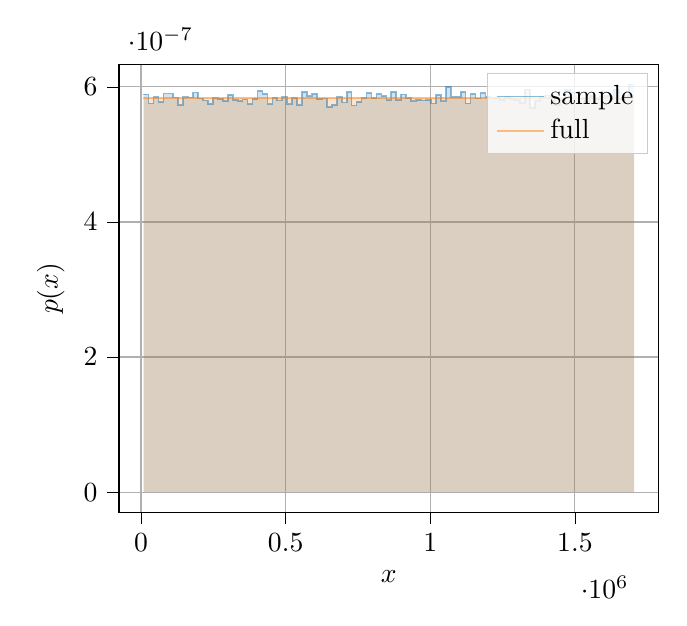
\begin{tikzpicture}

\definecolor{color0}{rgb}{0.12156862745098,0.466666666666667,0.705882352941177}
\definecolor{color1}{rgb}{1,0.498039215686275,0.0549019607843137}

\begin{axis}[
legend cell align={left},
legend style={
  fill opacity=0.8,
  draw opacity=1,
  text opacity=1,
  %at={(0.03,0.03)},
  anchor=north east,
  draw=white!80!black
},
trim axis left,trim axis right,
tick align=outside,
tick pos=left,
%title={n\_rels=2, n\_samps=10000, p=50, alg='groupjoin', stat=0.0012, pval=0.3912},
x grid style={white!69.0196078431373!black},
xmajorgrids,
xmin=-76238.87125, xmax=1789470.82625,
xtick style={color=black},
xlabel={\(\displaystyle x\)},
ylabel={\(\displaystyle p(x)\)},
y grid style={white!69.0196078431373!black},
ymajorgrids,
ymin=-3.01687964448078e-08, ymax=6.33544725340965e-07,
ytick style={color=black},
ylabel near ticks
]
\path [fill=color0, fill opacity=0.2]
(axis cs:8566.115,0)
--(axis cs:8566.115,5.89748014070721e-07)
--(axis cs:8566.115,5.88862199607067e-07)
--(axis cs:25698.345,5.88862199607067e-07)
--(axis cs:25698.345,5.75166145207504e-07)
--(axis cs:42830.575,5.75166145207504e-07)
--(axis cs:42830.575,5.85046383455945e-07)
--(axis cs:59962.805,5.85046383455945e-07)
--(axis cs:59962.805,5.77823588598465e-07)
--(axis cs:77095.035,5.77823588598465e-07)
--(axis cs:77095.035,5.89952432793102e-07)
--(axis cs:94227.265,5.89952432793102e-07)
--(axis cs:94227.265,5.90156851515484e-07)
--(axis cs:111359.495,5.90156851515484e-07)
--(axis cs:111359.495,5.84433127288801e-07)
--(axis cs:128491.725,5.84433127288801e-07)
--(axis cs:128491.725,5.73190097557816e-07)
--(axis cs:145623.955,5.73190097557816e-07)
--(axis cs:145623.955,5.84841964733564e-07)
--(axis cs:162756.185,5.84841964733564e-07)
--(axis cs:162756.185,5.84364987714673e-07)
--(axis cs:179888.415,5.84364987714673e-07)
--(axis cs:179888.415,5.914515034239e-07)
--(axis cs:197020.645,5.914515034239e-07)
--(axis cs:197020.645,5.82865917083876e-07)
--(axis cs:214152.875,5.82865917083876e-07)
--(axis cs:214152.875,5.79867775822279e-07)
--(axis cs:231285.105,5.79867775822279e-07)
--(axis cs:231285.105,5.75029866059251e-07)
--(axis cs:248417.335,5.75029866059251e-07)
--(axis cs:248417.335,5.83683591973401e-07)
--(axis cs:265549.565,5.83683591973401e-07)
--(axis cs:265549.565,5.81843823471969e-07)
--(axis cs:282681.795,5.81843823471969e-07)
--(axis cs:282681.795,5.79254519655134e-07)
--(axis cs:299814.025,5.79254519655134e-07)
--(axis cs:299814.025,5.88112664291669e-07)
--(axis cs:316946.255,5.88112664291669e-07)
--(axis cs:316946.255,5.81026148582442e-07)
--(axis cs:334078.485,5.81026148582442e-07)
--(axis cs:334078.485,5.79050100932752e-07)
--(axis cs:351210.715,5.79050100932752e-07)
--(axis cs:351210.715,5.8109428815657e-07)
--(axis cs:368342.945,5.8109428815657e-07)
--(axis cs:368342.945,5.74212191169725e-07)
--(axis cs:385475.175,5.74212191169725e-07)
--(axis cs:385475.175,5.82048242194348e-07)
--(axis cs:402607.405,5.82048242194348e-07)
--(axis cs:402607.405,5.94108946814861e-07)
--(axis cs:419739.635,5.94108946814861e-07)
--(axis cs:419739.635,5.89748014070721e-07)
--(axis cs:436871.865,5.89748014070721e-07)
--(axis cs:436871.865,5.74144051595598e-07)
--(axis cs:454004.095,5.74144051595598e-07)
--(axis cs:454004.095,5.83956150269909e-07)
--(axis cs:471136.325,5.83956150269909e-07)
--(axis cs:471136.325,5.7986777582228e-07)
--(axis cs:488268.555,5.7986777582228e-07)
--(axis cs:488268.555,5.84569406437056e-07)
--(axis cs:505400.785,5.84569406437056e-07)
--(axis cs:505400.785,5.74144051595596e-07)
--(axis cs:522533.015,5.74144051595596e-07)
--(axis cs:522533.015,5.83206614954512e-07)
--(axis cs:539665.245,5.83206614954512e-07)
--(axis cs:539665.245,5.73326376706071e-07)
--(axis cs:556797.475,5.73326376706071e-07)
--(axis cs:556797.475,5.9267801575819e-07)
--(axis cs:573929.705,5.9267801575819e-07)
--(axis cs:573929.705,5.86681733234998e-07)
--(axis cs:591061.935,5.86681733234998e-07)
--(axis cs:591061.935,5.892028974777e-07)
--(axis cs:608194.165,5.892028974777e-07)
--(axis cs:608194.165,5.82320800490859e-07)
--(axis cs:625326.395,5.82320800490859e-07)
--(axis cs:625326.395,5.82593358787368e-07)
--(axis cs:642458.625,5.82593358787368e-07)
--(axis cs:642458.625,5.6998753757384e-07)
--(axis cs:659590.855,5.6998753757384e-07)
--(axis cs:659590.855,5.73053818409563e-07)
--(axis cs:676723.085,5.73053818409563e-07)
--(axis cs:676723.085,5.851826626042e-07)
--(axis cs:693855.315,5.851826626042e-07)
--(axis cs:693855.315,5.77005913708935e-07)
--(axis cs:710987.545,5.77005913708935e-07)
--(axis cs:710987.545,5.92337317887554e-07)
--(axis cs:728119.775,5.92337317887554e-07)
--(axis cs:728119.775,5.72440562242418e-07)
--(axis cs:745252.005,5.72440562242418e-07)
--(axis cs:745252.005,5.78028007320847e-07)
--(axis cs:762384.235,5.78028007320847e-07)
--(axis cs:762384.235,5.83956150269911e-07)
--(axis cs:779516.465,5.83956150269911e-07)
--(axis cs:779516.465,5.91110805553265e-07)
--(axis cs:796648.695,5.91110805553265e-07)
--(axis cs:796648.695,5.83479173251017e-07)
--(axis cs:813780.925,5.83479173251017e-07)
--(axis cs:813780.925,5.88998478755322e-07)
--(axis cs:830913.155,5.88998478755322e-07)
--(axis cs:830913.155,5.86204756216108e-07)
--(axis cs:848045.385,5.86204756216108e-07)
--(axis cs:848045.385,5.80412892415298e-07)
--(axis cs:865177.615,5.80412892415298e-07)
--(axis cs:865177.615,5.92405457461681e-07)
--(axis cs:882309.845,5.92405457461681e-07)
--(axis cs:882309.845,5.80958009008315e-07)
--(axis cs:899442.075,5.80958009008315e-07)
--(axis cs:899442.075,5.88725920458813e-07)
--(axis cs:916574.305,5.88725920458813e-07)
--(axis cs:916574.305,5.8341103367689e-07)
--(axis cs:933706.535,5.8341103367689e-07)
--(axis cs:933706.535,5.78573123913864e-07)
--(axis cs:950838.765,5.78573123913864e-07)
--(axis cs:950838.765,5.80889869434188e-07)
--(axis cs:967970.995,5.80889869434188e-07)
--(axis cs:967970.995,5.7986777582228e-07)
--(axis cs:985103.225,5.7986777582228e-07)
--(axis cs:985103.225,5.80481031989425e-07)
--(axis cs:1002235.455,5.80481031989425e-07)
--(axis cs:1002235.455,5.75302424355759e-07)
--(axis cs:1019367.685,5.75302424355759e-07)
--(axis cs:1019367.685,5.87703826846902e-07)
--(axis cs:1036499.915,5.87703826846902e-07)
--(axis cs:1036499.915,5.78573123913864e-07)
--(axis cs:1053632.145,5.78573123913864e-07)
--(axis cs:1053632.145,6.00241508486306e-07)
--(axis cs:1070764.375,6.00241508486306e-07)
--(axis cs:1070764.375,5.85387081326582e-07)
--(axis cs:1087896.605,5.85387081326582e-07)
--(axis cs:1087896.605,5.85455220900709e-07)
--(axis cs:1105028.835,5.85455220900709e-07)
--(axis cs:1105028.835,5.92269178313427e-07)
--(axis cs:1122161.065,5.92269178313427e-07)
--(axis cs:1122161.065,5.75574982652268e-07)
--(axis cs:1139293.295,5.75574982652268e-07)
--(axis cs:1139293.295,5.89407316200085e-07)
--(axis cs:1156425.525,5.89407316200085e-07)
--(axis cs:1156425.525,5.82661498361495e-07)
--(axis cs:1173557.755,5.82661498361495e-07)
--(axis cs:1173557.755,5.90429409811993e-07)
--(axis cs:1190689.985,5.90429409811993e-07)
--(axis cs:1190689.985,5.84978243881811e-07)
--(axis cs:1207822.215,5.84978243881811e-07)
--(axis cs:1207822.215,5.84296848140547e-07)
--(axis cs:1224954.445,5.84296848140547e-07)
--(axis cs:1224954.445,5.8375173154753e-07)
--(axis cs:1242086.675,5.8375173154753e-07)
--(axis cs:1242086.675,5.80276613267043e-07)
--(axis cs:1259218.905,5.80276613267043e-07)
--(axis cs:1259218.905,5.8470568558531e-07)
--(axis cs:1276351.135,5.8470568558531e-07)
--(axis cs:1276351.135,5.8157126517546e-07)
--(axis cs:1293483.365,5.8157126517546e-07)
--(axis cs:1293483.365,5.81026148582442e-07)
--(axis cs:1310615.595,5.81026148582442e-07)
--(axis cs:1310615.595,5.76460797115922e-07)
--(axis cs:1327747.825,5.76460797115922e-07)
--(axis cs:1327747.825,5.9628941318693e-07)
--(axis cs:1344880.055,5.9628941318693e-07)
--(axis cs:1344880.055,5.68624746091296e-07)
--(axis cs:1362012.285,5.68624746091296e-07)
--(axis cs:1362012.285,5.789138217845e-07)
--(axis cs:1379144.515,5.789138217845e-07)
--(axis cs:1379144.515,5.84569406437056e-07)
--(axis cs:1396276.745,5.84569406437056e-07)
--(axis cs:1396276.745,5.87294989402143e-07)
--(axis cs:1413408.975,5.87294989402143e-07)
--(axis cs:1413408.975,5.83819871121649e-07)
--(axis cs:1430541.205,5.83819871121649e-07)
--(axis cs:1430541.205,5.73326376706071e-07)
--(axis cs:1447673.435,5.73326376706071e-07)
--(axis cs:1447673.435,5.81026148582442e-07)
--(axis cs:1464805.665,5.81026148582442e-07)
--(axis cs:1464805.665,5.9628941318693e-07)
--(axis cs:1481937.895,5.9628941318693e-07)
--(axis cs:1481937.895,5.91724061720409e-07)
--(axis cs:1499070.125,5.91724061720409e-07)
--(axis cs:1499070.125,5.91315224275646e-07)
--(axis cs:1516202.355,5.91315224275646e-07)
--(axis cs:1516202.355,5.82865917083876e-07)
--(axis cs:1533334.585,5.82865917083876e-07)
--(axis cs:1533334.585,5.7843684476561e-07)
--(axis cs:1550466.815,5.7843684476561e-07)
--(axis cs:1550466.815,5.86272895790235e-07)
--(axis cs:1567599.045,5.86272895790235e-07)
--(axis cs:1567599.045,5.82252660916732e-07)
--(axis cs:1584731.275,5.82252660916732e-07)
--(axis cs:1584731.275,5.86749872809125e-07)
--(axis cs:1601863.505,5.86749872809125e-07)
--(axis cs:1601863.505,5.86000337493726e-07)
--(axis cs:1618995.735,5.86000337493726e-07)
--(axis cs:1618995.735,5.85864058345464e-07)
--(axis cs:1636127.965,5.85864058345464e-07)
--(axis cs:1636127.965,5.95539877871531e-07)
--(axis cs:1653260.195,5.95539877871531e-07)
--(axis cs:1653260.195,5.8109428815657e-07)
--(axis cs:1670392.425,5.8109428815657e-07)
--(axis cs:1670392.425,5.86613593660871e-07)
--(axis cs:1687524.655,5.86613593660871e-07)
--(axis cs:1687524.655,6.03375928896157e-07)
--(axis cs:1704656.885,6.03375928896157e-07)
--(axis cs:1704656.885,0)
--(axis cs:1704656.885,0)
--(axis cs:1687524.655,0)
--(axis cs:1687524.655,0)
--(axis cs:1670392.425,0)
--(axis cs:1670392.425,0)
--(axis cs:1653260.195,0)
--(axis cs:1653260.195,0)
--(axis cs:1636127.965,0)
--(axis cs:1636127.965,0)
--(axis cs:1618995.735,0)
--(axis cs:1618995.735,0)
--(axis cs:1601863.505,0)
--(axis cs:1601863.505,0)
--(axis cs:1584731.275,0)
--(axis cs:1584731.275,0)
--(axis cs:1567599.045,0)
--(axis cs:1567599.045,0)
--(axis cs:1550466.815,0)
--(axis cs:1550466.815,0)
--(axis cs:1533334.585,0)
--(axis cs:1533334.585,0)
--(axis cs:1516202.355,0)
--(axis cs:1516202.355,0)
--(axis cs:1499070.125,0)
--(axis cs:1499070.125,0)
--(axis cs:1481937.895,0)
--(axis cs:1481937.895,0)
--(axis cs:1464805.665,0)
--(axis cs:1464805.665,0)
--(axis cs:1447673.435,0)
--(axis cs:1447673.435,0)
--(axis cs:1430541.205,0)
--(axis cs:1430541.205,0)
--(axis cs:1413408.975,0)
--(axis cs:1413408.975,0)
--(axis cs:1396276.745,0)
--(axis cs:1396276.745,0)
--(axis cs:1379144.515,0)
--(axis cs:1379144.515,0)
--(axis cs:1362012.285,0)
--(axis cs:1362012.285,0)
--(axis cs:1344880.055,0)
--(axis cs:1344880.055,0)
--(axis cs:1327747.825,0)
--(axis cs:1327747.825,0)
--(axis cs:1310615.595,0)
--(axis cs:1310615.595,0)
--(axis cs:1293483.365,0)
--(axis cs:1293483.365,0)
--(axis cs:1276351.135,0)
--(axis cs:1276351.135,0)
--(axis cs:1259218.905,0)
--(axis cs:1259218.905,0)
--(axis cs:1242086.675,0)
--(axis cs:1242086.675,0)
--(axis cs:1224954.445,0)
--(axis cs:1224954.445,0)
--(axis cs:1207822.215,0)
--(axis cs:1207822.215,0)
--(axis cs:1190689.985,0)
--(axis cs:1190689.985,0)
--(axis cs:1173557.755,0)
--(axis cs:1173557.755,0)
--(axis cs:1156425.525,0)
--(axis cs:1156425.525,0)
--(axis cs:1139293.295,0)
--(axis cs:1139293.295,0)
--(axis cs:1122161.065,0)
--(axis cs:1122161.065,0)
--(axis cs:1105028.835,0)
--(axis cs:1105028.835,0)
--(axis cs:1087896.605,0)
--(axis cs:1087896.605,0)
--(axis cs:1070764.375,0)
--(axis cs:1070764.375,0)
--(axis cs:1053632.145,0)
--(axis cs:1053632.145,0)
--(axis cs:1036499.915,0)
--(axis cs:1036499.915,0)
--(axis cs:1019367.685,0)
--(axis cs:1019367.685,0)
--(axis cs:1002235.455,0)
--(axis cs:1002235.455,0)
--(axis cs:985103.225,0)
--(axis cs:985103.225,0)
--(axis cs:967970.995,0)
--(axis cs:967970.995,0)
--(axis cs:950838.765,0)
--(axis cs:950838.765,0)
--(axis cs:933706.535,0)
--(axis cs:933706.535,0)
--(axis cs:916574.305,0)
--(axis cs:916574.305,0)
--(axis cs:899442.075,0)
--(axis cs:899442.075,0)
--(axis cs:882309.845,0)
--(axis cs:882309.845,0)
--(axis cs:865177.615,0)
--(axis cs:865177.615,0)
--(axis cs:848045.385,0)
--(axis cs:848045.385,0)
--(axis cs:830913.155,0)
--(axis cs:830913.155,0)
--(axis cs:813780.925,0)
--(axis cs:813780.925,0)
--(axis cs:796648.695,0)
--(axis cs:796648.695,0)
--(axis cs:779516.465,0)
--(axis cs:779516.465,0)
--(axis cs:762384.235,0)
--(axis cs:762384.235,0)
--(axis cs:745252.005,0)
--(axis cs:745252.005,0)
--(axis cs:728119.775,0)
--(axis cs:728119.775,0)
--(axis cs:710987.545,0)
--(axis cs:710987.545,0)
--(axis cs:693855.315,0)
--(axis cs:693855.315,0)
--(axis cs:676723.085,0)
--(axis cs:676723.085,0)
--(axis cs:659590.855,0)
--(axis cs:659590.855,0)
--(axis cs:642458.625,0)
--(axis cs:642458.625,0)
--(axis cs:625326.395,0)
--(axis cs:625326.395,0)
--(axis cs:608194.165,0)
--(axis cs:608194.165,0)
--(axis cs:591061.935,0)
--(axis cs:591061.935,0)
--(axis cs:573929.705,0)
--(axis cs:573929.705,0)
--(axis cs:556797.475,0)
--(axis cs:556797.475,0)
--(axis cs:539665.245,0)
--(axis cs:539665.245,0)
--(axis cs:522533.015,0)
--(axis cs:522533.015,0)
--(axis cs:505400.785,0)
--(axis cs:505400.785,0)
--(axis cs:488268.555,0)
--(axis cs:488268.555,0)
--(axis cs:471136.325,0)
--(axis cs:471136.325,0)
--(axis cs:454004.095,0)
--(axis cs:454004.095,0)
--(axis cs:436871.865,0)
--(axis cs:436871.865,0)
--(axis cs:419739.635,0)
--(axis cs:419739.635,0)
--(axis cs:402607.405,0)
--(axis cs:402607.405,0)
--(axis cs:385475.175,0)
--(axis cs:385475.175,0)
--(axis cs:368342.945,0)
--(axis cs:368342.945,0)
--(axis cs:351210.715,0)
--(axis cs:351210.715,0)
--(axis cs:334078.485,0)
--(axis cs:334078.485,0)
--(axis cs:316946.255,0)
--(axis cs:316946.255,0)
--(axis cs:299814.025,0)
--(axis cs:299814.025,0)
--(axis cs:282681.795,0)
--(axis cs:282681.795,0)
--(axis cs:265549.565,0)
--(axis cs:265549.565,0)
--(axis cs:248417.335,0)
--(axis cs:248417.335,0)
--(axis cs:231285.105,0)
--(axis cs:231285.105,0)
--(axis cs:214152.875,0)
--(axis cs:214152.875,0)
--(axis cs:197020.645,0)
--(axis cs:197020.645,0)
--(axis cs:179888.415,0)
--(axis cs:179888.415,0)
--(axis cs:162756.185,0)
--(axis cs:162756.185,0)
--(axis cs:145623.955,0)
--(axis cs:145623.955,0)
--(axis cs:128491.725,0)
--(axis cs:128491.725,0)
--(axis cs:111359.495,0)
--(axis cs:111359.495,0)
--(axis cs:94227.265,0)
--(axis cs:94227.265,0)
--(axis cs:77095.035,0)
--(axis cs:77095.035,0)
--(axis cs:59962.805,0)
--(axis cs:59962.805,0)
--(axis cs:42830.575,0)
--(axis cs:42830.575,0)
--(axis cs:25698.345,0)
--(axis cs:25698.345,0)
--(axis cs:8566.115,0)
--(axis cs:8566.115,0)
--cycle;

\path [fill=color1, fill opacity=0.2]
(axis cs:8566.16,0)
--(axis cs:8566.16,5.8371493606733e-07)
--(axis cs:8566.16,5.83680866439357e-07)
--(axis cs:25698.48,5.83680866439357e-07)
--(axis cs:25698.48,5.83680866439357e-07)
--(axis cs:42830.8,5.83680866439357e-07)
--(axis cs:42830.8,5.8371493606733e-07)
--(axis cs:59963.12,5.8371493606733e-07)
--(axis cs:59963.12,5.83680866439357e-07)
--(axis cs:77095.44,5.83680866439357e-07)
--(axis cs:77095.44,5.83680866439357e-07)
--(axis cs:94227.76,5.83680866439357e-07)
--(axis cs:94227.76,5.83714936067331e-07)
--(axis cs:111360.08,5.83714936067331e-07)
--(axis cs:111360.08,5.83680866439357e-07)
--(axis cs:128492.4,5.83680866439357e-07)
--(axis cs:128492.4,5.83680866439357e-07)
--(axis cs:145624.72,5.83680866439357e-07)
--(axis cs:145624.72,5.8371493606733e-07)
--(axis cs:162757.04,5.8371493606733e-07)
--(axis cs:162757.04,5.83680866439358e-07)
--(axis cs:179889.36,5.83680866439358e-07)
--(axis cs:179889.36,5.83680866439357e-07)
--(axis cs:197021.68,5.83680866439357e-07)
--(axis cs:197021.68,5.8371493606733e-07)
--(axis cs:214154,5.8371493606733e-07)
--(axis cs:214154,5.83680866439358e-07)
--(axis cs:231286.32,5.83680866439358e-07)
--(axis cs:231286.32,5.83680866439357e-07)
--(axis cs:248418.64,5.83680866439357e-07)
--(axis cs:248418.64,5.8371493606733e-07)
--(axis cs:265550.96,5.8371493606733e-07)
--(axis cs:265550.96,5.83680866439357e-07)
--(axis cs:282683.28,5.83680866439357e-07)
--(axis cs:282683.28,5.83680866439357e-07)
--(axis cs:299815.6,5.83680866439357e-07)
--(axis cs:299815.6,5.8371493606733e-07)
--(axis cs:316947.92,5.8371493606733e-07)
--(axis cs:316947.92,5.83680866439357e-07)
--(axis cs:334080.24,5.83680866439357e-07)
--(axis cs:334080.24,5.83680866439359e-07)
--(axis cs:351212.56,5.83680866439359e-07)
--(axis cs:351212.56,5.8371493606733e-07)
--(axis cs:368344.88,5.8371493606733e-07)
--(axis cs:368344.88,5.83680866439357e-07)
--(axis cs:385477.2,5.83680866439357e-07)
--(axis cs:385477.2,5.83680866439357e-07)
--(axis cs:402609.52,5.83680866439357e-07)
--(axis cs:402609.52,5.83680866439357e-07)
--(axis cs:419741.84,5.83680866439357e-07)
--(axis cs:419741.84,5.8371493606733e-07)
--(axis cs:436874.16,5.8371493606733e-07)
--(axis cs:436874.16,5.83680866439357e-07)
--(axis cs:454006.48,5.83680866439357e-07)
--(axis cs:454006.48,5.83680866439359e-07)
--(axis cs:471138.8,5.83680866439359e-07)
--(axis cs:471138.8,5.8371493606733e-07)
--(axis cs:488271.12,5.8371493606733e-07)
--(axis cs:488271.12,5.83680866439357e-07)
--(axis cs:505403.44,5.83680866439357e-07)
--(axis cs:505403.44,5.83680866439355e-07)
--(axis cs:522535.76,5.83680866439355e-07)
--(axis cs:522535.76,5.83714936067332e-07)
--(axis cs:539668.08,5.83714936067332e-07)
--(axis cs:539668.08,5.83680866439359e-07)
--(axis cs:556800.4,5.83680866439359e-07)
--(axis cs:556800.4,5.83680866439355e-07)
--(axis cs:573932.72,5.83680866439355e-07)
--(axis cs:573932.72,5.83714936067332e-07)
--(axis cs:591065.04,5.83714936067332e-07)
--(axis cs:591065.04,5.83680866439355e-07)
--(axis cs:608197.36,5.83680866439355e-07)
--(axis cs:608197.36,5.83680866439359e-07)
--(axis cs:625329.68,5.83680866439359e-07)
--(axis cs:625329.68,5.83714936067328e-07)
--(axis cs:642462,5.83714936067328e-07)
--(axis cs:642462,5.83680866439359e-07)
--(axis cs:659594.32,5.83680866439359e-07)
--(axis cs:659594.32,5.83680866439355e-07)
--(axis cs:676726.64,5.83680866439355e-07)
--(axis cs:676726.64,5.83714936067332e-07)
--(axis cs:693858.96,5.83714936067332e-07)
--(axis cs:693858.96,5.83680866439359e-07)
--(axis cs:710991.28,5.83680866439359e-07)
--(axis cs:710991.28,5.83680866439355e-07)
--(axis cs:728123.6,5.83680866439355e-07)
--(axis cs:728123.6,5.83714936067332e-07)
--(axis cs:745255.92,5.83714936067332e-07)
--(axis cs:745255.92,5.83680866439355e-07)
--(axis cs:762388.24,5.83680866439355e-07)
--(axis cs:762388.24,5.83680866439359e-07)
--(axis cs:779520.56,5.83680866439359e-07)
--(axis cs:779520.56,5.83714936067328e-07)
--(axis cs:796652.88,5.83714936067328e-07)
--(axis cs:796652.88,5.83680866439359e-07)
--(axis cs:813785.2,5.83680866439359e-07)
--(axis cs:813785.2,5.83680866439359e-07)
--(axis cs:830917.52,5.83680866439359e-07)
--(axis cs:830917.52,5.83680866439355e-07)
--(axis cs:848049.84,5.83680866439355e-07)
--(axis cs:848049.84,5.83714936067332e-07)
--(axis cs:865182.16,5.83714936067332e-07)
--(axis cs:865182.16,5.83680866439355e-07)
--(axis cs:882314.48,5.83680866439355e-07)
--(axis cs:882314.48,5.83680866439359e-07)
--(axis cs:899446.8,5.83680866439359e-07)
--(axis cs:899446.8,5.83714936067328e-07)
--(axis cs:916579.12,5.83714936067328e-07)
--(axis cs:916579.12,5.83680866439359e-07)
--(axis cs:933711.44,5.83680866439359e-07)
--(axis cs:933711.44,5.83680866439359e-07)
--(axis cs:950843.76,5.83680866439359e-07)
--(axis cs:950843.76,5.83714936067328e-07)
--(axis cs:967976.08,5.83714936067328e-07)
--(axis cs:967976.08,5.83680866439359e-07)
--(axis cs:985108.4,5.83680866439359e-07)
--(axis cs:985108.4,5.83680866439355e-07)
--(axis cs:1002240.72,5.83680866439355e-07)
--(axis cs:1002240.72,5.83714936067332e-07)
--(axis cs:1019373.04,5.83714936067332e-07)
--(axis cs:1019373.04,5.83680866439355e-07)
--(axis cs:1036505.36,5.83680866439355e-07)
--(axis cs:1036505.36,5.83680866439355e-07)
--(axis cs:1053637.68,5.83680866439355e-07)
--(axis cs:1053637.68,5.83714936067336e-07)
--(axis cs:1070770,5.83714936067336e-07)
--(axis cs:1070770,5.83680866439355e-07)
--(axis cs:1087902.32,5.83680866439355e-07)
--(axis cs:1087902.32,5.83680866439355e-07)
--(axis cs:1105034.64,5.83680866439355e-07)
--(axis cs:1105034.64,5.83714936067336e-07)
--(axis cs:1122166.96,5.83714936067336e-07)
--(axis cs:1122166.96,5.83680866439355e-07)
--(axis cs:1139299.28,5.83680866439355e-07)
--(axis cs:1139299.28,5.83680866439355e-07)
--(axis cs:1156431.6,5.83680866439355e-07)
--(axis cs:1156431.6,5.83714936067328e-07)
--(axis cs:1173563.92,5.83714936067328e-07)
--(axis cs:1173563.92,5.83680866439363e-07)
--(axis cs:1190696.24,5.83680866439363e-07)
--(axis cs:1190696.24,5.83680866439355e-07)
--(axis cs:1207828.56,5.83680866439355e-07)
--(axis cs:1207828.56,5.83714936067328e-07)
--(axis cs:1224960.88,5.83714936067328e-07)
--(axis cs:1224960.88,5.83680866439363e-07)
--(axis cs:1242093.2,5.83680866439363e-07)
--(axis cs:1242093.2,5.83680866439355e-07)
--(axis cs:1259225.52,5.83680866439355e-07)
--(axis cs:1259225.52,5.83680866439355e-07)
--(axis cs:1276357.84,5.83680866439355e-07)
--(axis cs:1276357.84,5.83714936067328e-07)
--(axis cs:1293490.16,5.83714936067328e-07)
--(axis cs:1293490.16,5.83680866439363e-07)
--(axis cs:1310622.48,5.83680866439363e-07)
--(axis cs:1310622.48,5.83680866439355e-07)
--(axis cs:1327754.8,5.83680866439355e-07)
--(axis cs:1327754.8,5.83714936067328e-07)
--(axis cs:1344887.12,5.83714936067328e-07)
--(axis cs:1344887.12,5.83680866439355e-07)
--(axis cs:1362019.44,5.83680866439355e-07)
--(axis cs:1362019.44,5.83680866439363e-07)
--(axis cs:1379151.76,5.83680866439363e-07)
--(axis cs:1379151.76,5.83714936067328e-07)
--(axis cs:1396284.08,5.83714936067328e-07)
--(axis cs:1396284.08,5.83680866439355e-07)
--(axis cs:1413416.4,5.83680866439355e-07)
--(axis cs:1413416.4,5.83680866439363e-07)
--(axis cs:1430548.72,5.83680866439363e-07)
--(axis cs:1430548.72,5.83714936067328e-07)
--(axis cs:1447681.04,5.83714936067328e-07)
--(axis cs:1447681.04,5.83680866439355e-07)
--(axis cs:1464813.36,5.83680866439355e-07)
--(axis cs:1464813.36,5.83680866439355e-07)
--(axis cs:1481945.68,5.83680866439355e-07)
--(axis cs:1481945.68,5.83714936067336e-07)
--(axis cs:1499078,5.83714936067336e-07)
--(axis cs:1499078,5.83680866439355e-07)
--(axis cs:1516210.32,5.83680866439355e-07)
--(axis cs:1516210.32,5.83680866439355e-07)
--(axis cs:1533342.64,5.83680866439355e-07)
--(axis cs:1533342.64,5.83714936067336e-07)
--(axis cs:1550474.96,5.83714936067336e-07)
--(axis cs:1550474.96,5.83680866439355e-07)
--(axis cs:1567607.28,5.83680866439355e-07)
--(axis cs:1567607.28,5.83680866439355e-07)
--(axis cs:1584739.6,5.83680866439355e-07)
--(axis cs:1584739.6,5.83714936067328e-07)
--(axis cs:1601871.92,5.83714936067328e-07)
--(axis cs:1601871.92,5.83680866439363e-07)
--(axis cs:1619004.24,5.83680866439363e-07)
--(axis cs:1619004.24,5.83680866439355e-07)
--(axis cs:1636136.56,5.83680866439355e-07)
--(axis cs:1636136.56,5.83714936067328e-07)
--(axis cs:1653268.88,5.83714936067328e-07)
--(axis cs:1653268.88,5.83680866439363e-07)
--(axis cs:1670401.2,5.83680866439363e-07)
--(axis cs:1670401.2,5.83680866439355e-07)
--(axis cs:1687533.52,5.83680866439355e-07)
--(axis cs:1687533.52,5.83714936067328e-07)
--(axis cs:1704665.84,5.83714936067328e-07)
--(axis cs:1704665.84,0)
--(axis cs:1704665.84,0)
--(axis cs:1687533.52,0)
--(axis cs:1687533.52,0)
--(axis cs:1670401.2,0)
--(axis cs:1670401.2,0)
--(axis cs:1653268.88,0)
--(axis cs:1653268.88,0)
--(axis cs:1636136.56,0)
--(axis cs:1636136.56,0)
--(axis cs:1619004.24,0)
--(axis cs:1619004.24,0)
--(axis cs:1601871.92,0)
--(axis cs:1601871.92,0)
--(axis cs:1584739.6,0)
--(axis cs:1584739.6,0)
--(axis cs:1567607.28,0)
--(axis cs:1567607.28,0)
--(axis cs:1550474.96,0)
--(axis cs:1550474.96,0)
--(axis cs:1533342.64,0)
--(axis cs:1533342.64,0)
--(axis cs:1516210.32,0)
--(axis cs:1516210.32,0)
--(axis cs:1499078,0)
--(axis cs:1499078,0)
--(axis cs:1481945.68,0)
--(axis cs:1481945.68,0)
--(axis cs:1464813.36,0)
--(axis cs:1464813.36,0)
--(axis cs:1447681.04,0)
--(axis cs:1447681.04,0)
--(axis cs:1430548.72,0)
--(axis cs:1430548.72,0)
--(axis cs:1413416.4,0)
--(axis cs:1413416.4,0)
--(axis cs:1396284.08,0)
--(axis cs:1396284.08,0)
--(axis cs:1379151.76,0)
--(axis cs:1379151.76,0)
--(axis cs:1362019.44,0)
--(axis cs:1362019.44,0)
--(axis cs:1344887.12,0)
--(axis cs:1344887.12,0)
--(axis cs:1327754.8,0)
--(axis cs:1327754.8,0)
--(axis cs:1310622.48,0)
--(axis cs:1310622.48,0)
--(axis cs:1293490.16,0)
--(axis cs:1293490.16,0)
--(axis cs:1276357.84,0)
--(axis cs:1276357.84,0)
--(axis cs:1259225.52,0)
--(axis cs:1259225.52,0)
--(axis cs:1242093.2,0)
--(axis cs:1242093.2,0)
--(axis cs:1224960.88,0)
--(axis cs:1224960.88,0)
--(axis cs:1207828.56,0)
--(axis cs:1207828.56,0)
--(axis cs:1190696.24,0)
--(axis cs:1190696.24,0)
--(axis cs:1173563.92,0)
--(axis cs:1173563.92,0)
--(axis cs:1156431.6,0)
--(axis cs:1156431.6,0)
--(axis cs:1139299.28,0)
--(axis cs:1139299.28,0)
--(axis cs:1122166.96,0)
--(axis cs:1122166.96,0)
--(axis cs:1105034.64,0)
--(axis cs:1105034.64,0)
--(axis cs:1087902.32,0)
--(axis cs:1087902.32,0)
--(axis cs:1070770,0)
--(axis cs:1070770,0)
--(axis cs:1053637.68,0)
--(axis cs:1053637.68,0)
--(axis cs:1036505.36,0)
--(axis cs:1036505.36,0)
--(axis cs:1019373.04,0)
--(axis cs:1019373.04,0)
--(axis cs:1002240.72,0)
--(axis cs:1002240.72,0)
--(axis cs:985108.4,0)
--(axis cs:985108.4,0)
--(axis cs:967976.08,0)
--(axis cs:967976.08,0)
--(axis cs:950843.76,0)
--(axis cs:950843.76,0)
--(axis cs:933711.44,0)
--(axis cs:933711.44,0)
--(axis cs:916579.12,0)
--(axis cs:916579.12,0)
--(axis cs:899446.8,0)
--(axis cs:899446.8,0)
--(axis cs:882314.48,0)
--(axis cs:882314.48,0)
--(axis cs:865182.16,0)
--(axis cs:865182.16,0)
--(axis cs:848049.84,0)
--(axis cs:848049.84,0)
--(axis cs:830917.52,0)
--(axis cs:830917.52,0)
--(axis cs:813785.2,0)
--(axis cs:813785.2,0)
--(axis cs:796652.88,0)
--(axis cs:796652.88,0)
--(axis cs:779520.56,0)
--(axis cs:779520.56,0)
--(axis cs:762388.24,0)
--(axis cs:762388.24,0)
--(axis cs:745255.92,0)
--(axis cs:745255.92,0)
--(axis cs:728123.6,0)
--(axis cs:728123.6,0)
--(axis cs:710991.28,0)
--(axis cs:710991.28,0)
--(axis cs:693858.96,0)
--(axis cs:693858.96,0)
--(axis cs:676726.64,0)
--(axis cs:676726.64,0)
--(axis cs:659594.32,0)
--(axis cs:659594.32,0)
--(axis cs:642462,0)
--(axis cs:642462,0)
--(axis cs:625329.68,0)
--(axis cs:625329.68,0)
--(axis cs:608197.36,0)
--(axis cs:608197.36,0)
--(axis cs:591065.04,0)
--(axis cs:591065.04,0)
--(axis cs:573932.72,0)
--(axis cs:573932.72,0)
--(axis cs:556800.4,0)
--(axis cs:556800.4,0)
--(axis cs:539668.08,0)
--(axis cs:539668.08,0)
--(axis cs:522535.76,0)
--(axis cs:522535.76,0)
--(axis cs:505403.44,0)
--(axis cs:505403.44,0)
--(axis cs:488271.12,0)
--(axis cs:488271.12,0)
--(axis cs:471138.8,0)
--(axis cs:471138.8,0)
--(axis cs:454006.48,0)
--(axis cs:454006.48,0)
--(axis cs:436874.16,0)
--(axis cs:436874.16,0)
--(axis cs:419741.84,0)
--(axis cs:419741.84,0)
--(axis cs:402609.52,0)
--(axis cs:402609.52,0)
--(axis cs:385477.2,0)
--(axis cs:385477.2,0)
--(axis cs:368344.88,0)
--(axis cs:368344.88,0)
--(axis cs:351212.56,0)
--(axis cs:351212.56,0)
--(axis cs:334080.24,0)
--(axis cs:334080.24,0)
--(axis cs:316947.92,0)
--(axis cs:316947.92,0)
--(axis cs:299815.6,0)
--(axis cs:299815.6,0)
--(axis cs:282683.28,0)
--(axis cs:282683.28,0)
--(axis cs:265550.96,0)
--(axis cs:265550.96,0)
--(axis cs:248418.64,0)
--(axis cs:248418.64,0)
--(axis cs:231286.32,0)
--(axis cs:231286.32,0)
--(axis cs:214154,0)
--(axis cs:214154,0)
--(axis cs:197021.68,0)
--(axis cs:197021.68,0)
--(axis cs:179889.36,0)
--(axis cs:179889.36,0)
--(axis cs:162757.04,0)
--(axis cs:162757.04,0)
--(axis cs:145624.72,0)
--(axis cs:145624.72,0)
--(axis cs:128492.4,0)
--(axis cs:128492.4,0)
--(axis cs:111360.08,0)
--(axis cs:111360.08,0)
--(axis cs:94227.76,0)
--(axis cs:94227.76,0)
--(axis cs:77095.44,0)
--(axis cs:77095.44,0)
--(axis cs:59963.12,0)
--(axis cs:59963.12,0)
--(axis cs:42830.8,0)
--(axis cs:42830.8,0)
--(axis cs:25698.48,0)
--(axis cs:25698.48,0)
--(axis cs:8566.16,0)
--(axis cs:8566.16,0)
--cycle;

\addplot [semithick, color0, const plot mark right, opacity=0.5]
table {%
8566.115 5.89748014070721e-07
25698.345 5.88862199607067e-07
42830.575 5.75166145207504e-07
59962.805 5.85046383455945e-07
77095.035 5.77823588598465e-07
94227.265 5.89952432793102e-07
111359.495 5.90156851515484e-07
128491.725 5.84433127288801e-07
145623.955 5.73190097557816e-07
162756.185 5.84841964733564e-07
179888.415 5.84364987714673e-07
197020.645 5.914515034239e-07
214152.875 5.82865917083876e-07
231285.105 5.79867775822279e-07
248417.335 5.75029866059251e-07
265549.565 5.83683591973401e-07
282681.795 5.81843823471969e-07
299814.025 5.79254519655134e-07
316946.255 5.88112664291669e-07
334078.485 5.81026148582442e-07
351210.715 5.79050100932752e-07
368342.945 5.8109428815657e-07
385475.175 5.74212191169725e-07
402607.405 5.82048242194348e-07
419739.635 5.94108946814861e-07
436871.865 5.89748014070721e-07
454004.095 5.74144051595598e-07
471136.325 5.83956150269909e-07
488268.555 5.7986777582228e-07
505400.785 5.84569406437056e-07
522533.015 5.74144051595596e-07
539665.245 5.83206614954512e-07
556797.475 5.73326376706071e-07
573929.705 5.9267801575819e-07
591061.935 5.86681733234998e-07
608194.165 5.892028974777e-07
625326.395 5.82320800490859e-07
642458.625 5.82593358787368e-07
659590.855 5.6998753757384e-07
676723.085 5.73053818409563e-07
693855.315 5.851826626042e-07
710987.545 5.77005913708935e-07
728119.775 5.92337317887554e-07
745252.005 5.72440562242418e-07
762384.235 5.78028007320847e-07
779516.465 5.83956150269911e-07
796648.695 5.91110805553265e-07
813780.925 5.83479173251017e-07
830913.155 5.88998478755322e-07
848045.385 5.86204756216108e-07
865177.615 5.80412892415298e-07
882309.845 5.92405457461681e-07
899442.075 5.80958009008315e-07
916574.305 5.88725920458813e-07
933706.535 5.8341103367689e-07
950838.765 5.78573123913864e-07
967970.995 5.80889869434188e-07
985103.225 5.7986777582228e-07
1002235.455 5.80481031989425e-07
1019367.685 5.75302424355759e-07
1036499.915 5.87703826846902e-07
1053632.145 5.78573123913864e-07
1070764.375 6.00241508486306e-07
1087896.605 5.85387081326582e-07
1105028.835 5.85455220900709e-07
1122161.065 5.92269178313427e-07
1139293.295 5.75574982652268e-07
1156425.525 5.89407316200085e-07
1173557.755 5.82661498361495e-07
1190689.985 5.90429409811993e-07
1207822.215 5.84978243881811e-07
1224954.445 5.84296848140547e-07
1242086.675 5.8375173154753e-07
1259218.905 5.80276613267043e-07
1276351.135 5.8470568558531e-07
1293483.365 5.8157126517546e-07
1310615.595 5.81026148582442e-07
1327747.825 5.76460797115922e-07
1344880.055 5.9628941318693e-07
1362012.285 5.68624746091296e-07
1379144.515 5.789138217845e-07
1396276.745 5.84569406437056e-07
1413408.975 5.87294989402143e-07
1430541.205 5.83819871121649e-07
1447673.435 5.73326376706071e-07
1464805.665 5.81026148582442e-07
1481937.895 5.9628941318693e-07
1499070.125 5.91724061720409e-07
1516202.355 5.91315224275646e-07
1533334.585 5.82865917083876e-07
1550466.815 5.7843684476561e-07
1567599.045 5.86272895790235e-07
1584731.275 5.82252660916732e-07
1601863.505 5.86749872809125e-07
1618995.735 5.86000337493726e-07
1636127.965 5.85864058345464e-07
1653260.195 5.95539877871531e-07
1670392.425 5.8109428815657e-07
1687524.655 5.86613593660871e-07
1704656.885 6.03375928896157e-07
};
\addlegendentry{sample}
\addplot [semithick, color1, const plot mark right, opacity=0.5]
table {%
8566.16 5.8371493606733e-07
25698.48 5.83680866439357e-07
42830.8 5.83680866439357e-07
59963.12 5.8371493606733e-07
77095.44 5.83680866439357e-07
94227.76 5.83680866439357e-07
111360.08 5.83714936067331e-07
128492.4 5.83680866439357e-07
145624.72 5.83680866439357e-07
162757.04 5.8371493606733e-07
179889.36 5.83680866439358e-07
197021.68 5.83680866439357e-07
214154 5.8371493606733e-07
231286.32 5.83680866439358e-07
248418.64 5.83680866439357e-07
265550.96 5.8371493606733e-07
282683.28 5.83680866439357e-07
299815.6 5.83680866439357e-07
316947.92 5.8371493606733e-07
334080.24 5.83680866439357e-07
351212.56 5.83680866439359e-07
368344.88 5.8371493606733e-07
385477.2 5.83680866439357e-07
402609.52 5.83680866439357e-07
419741.84 5.83680866439357e-07
436874.16 5.8371493606733e-07
454006.48 5.83680866439357e-07
471138.8 5.83680866439359e-07
488271.12 5.8371493606733e-07
505403.44 5.83680866439357e-07
522535.76 5.83680866439355e-07
539668.08 5.83714936067332e-07
556800.4 5.83680866439359e-07
573932.72 5.83680866439355e-07
591065.04 5.83714936067332e-07
608197.36 5.83680866439355e-07
625329.68 5.83680866439359e-07
642462 5.83714936067328e-07
659594.32 5.83680866439359e-07
676726.64 5.83680866439355e-07
693858.96 5.83714936067332e-07
710991.28 5.83680866439359e-07
728123.6 5.83680866439355e-07
745255.92 5.83714936067332e-07
762388.24 5.83680866439355e-07
779520.56 5.83680866439359e-07
796652.88 5.83714936067328e-07
813785.2 5.83680866439359e-07
830917.52 5.83680866439359e-07
848049.84 5.83680866439355e-07
865182.16 5.83714936067332e-07
882314.48 5.83680866439355e-07
899446.8 5.83680866439359e-07
916579.12 5.83714936067328e-07
933711.44 5.83680866439359e-07
950843.76 5.83680866439359e-07
967976.08 5.83714936067328e-07
985108.4 5.83680866439359e-07
1002240.72 5.83680866439355e-07
1019373.04 5.83714936067332e-07
1036505.36 5.83680866439355e-07
1053637.68 5.83680866439355e-07
1070770 5.83714936067336e-07
1087902.32 5.83680866439355e-07
1105034.64 5.83680866439355e-07
1122166.96 5.83714936067336e-07
1139299.28 5.83680866439355e-07
1156431.6 5.83680866439355e-07
1173563.92 5.83714936067328e-07
1190696.24 5.83680866439363e-07
1207828.56 5.83680866439355e-07
1224960.88 5.83714936067328e-07
1242093.2 5.83680866439363e-07
1259225.52 5.83680866439355e-07
1276357.84 5.83680866439355e-07
1293490.16 5.83714936067328e-07
1310622.48 5.83680866439363e-07
1327754.8 5.83680866439355e-07
1344887.12 5.83714936067328e-07
1362019.44 5.83680866439355e-07
1379151.76 5.83680866439363e-07
1396284.08 5.83714936067328e-07
1413416.4 5.83680866439355e-07
1430548.72 5.83680866439363e-07
1447681.04 5.83714936067328e-07
1464813.36 5.83680866439355e-07
1481945.68 5.83680866439355e-07
1499078 5.83714936067336e-07
1516210.32 5.83680866439355e-07
1533342.64 5.83680866439355e-07
1550474.96 5.83714936067336e-07
1567607.28 5.83680866439355e-07
1584739.6 5.83680866439355e-07
1601871.92 5.83714936067328e-07
1619004.24 5.83680866439363e-07
1636136.56 5.83680866439355e-07
1653268.88 5.83714936067328e-07
1670401.2 5.83680866439363e-07
1687533.52 5.83680866439355e-07
1704665.84 5.83714936067328e-07
};
\addlegendentry{full}
\end{axis}

\end{tikzpicture}

	\end{adjustbox}}\medskip{}
\subfloat[KS tests for $n\protect\coloneqq10^{3},10^{4}$ and $f\protect\coloneqq0.1,\dots,0.9$.\label{fig:Group-join}]{    \centering
    \begin{adjustbox}{width=\linewidth,center}
    	% This file was created by tikzplotlib v0.9.8.
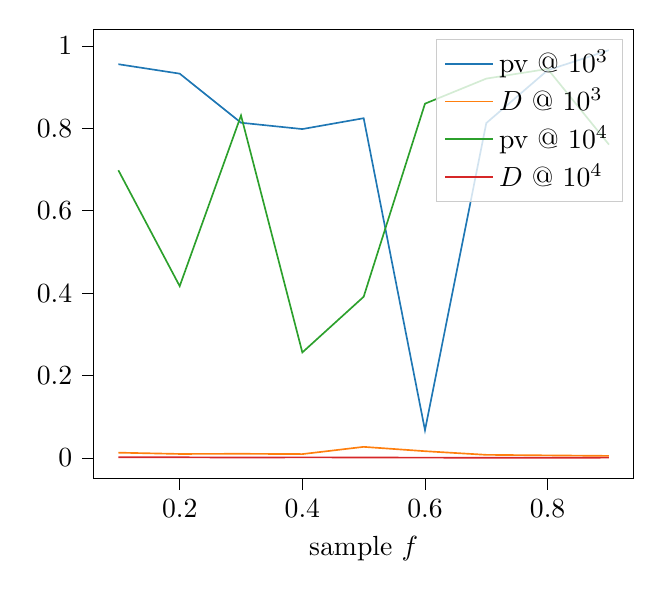
\begin{tikzpicture}

\definecolor{color0}{rgb}{0.12156862745098,0.466666666666667,0.705882352941177}
\definecolor{color1}{rgb}{1,0.498039215686275,0.0549019607843137}
\definecolor{color2}{rgb}{0.172549019607843,0.627450980392157,0.172549019607843}
\definecolor{color3}{rgb}{0.83921568627451,0.152941176470588,0.156862745098039}

\begin{axis}[
legend cell align={left},
legend style={fill opacity=0.8, draw opacity=1, text opacity=1, draw=white!80!black},
tick align=outside,
tick pos=left,
x grid style={white!69.0196078431373!black},
xlabel={sample \(\displaystyle f\)},
xmin=0.06, xmax=0.94,
xtick style={color=black},
y grid style={white!69.0196078431373!black},
ymin=-0.0488345314464655, ymax=1.03890625716295,
ytick style={color=black}
]
\addplot [semithick, color0]
table {%
0.1 0.955325423202725
0.2 0.932476404456486
0.3 0.813368343409041
0.4 0.798007103890111
0.5 0.824313005539974
0.6 0.0673680278852529
0.7 0.812600340553116
0.8 0.940750238300817
0.9 0.98946349404434
};
\addlegendentry{pv @ $10^3$}
\addplot [semithick, color1]
table {%
0.1 0.0128770212473673
0.2 0.00974352900079217
0.3 0.0101571005829238
0.4 0.00941132707515802
0.5 0.0269728274548857
0.6 0.0164403620186904
0.7 0.00759203805980968
0.8 0.00627739511584224
0.9 0.00505208250903266
};
\addlegendentry{$D$ @ $10^3$}
\addplot [semithick, color2]
table {%
0.1 0.698089266055995
0.2 0.416912825506407
0.3 0.83094039350407
0.4 0.256087252009837
0.5 0.391168038033697
0.6 0.859587909463171
0.7 0.920438283748443
0.8 0.94391275084072
0.9 0.760314916805552
};
\addlegendentry{pv @ $10^4$}
\addplot [semithick, color3]
table {%
0.1 0.00181762119824538
0.2 0.00165509783532602
0.3 0.00100063126812847
0.4 0.00146570335065871
0.5 0.00119216119738719
0.6 0.000755533512252327
0.7 0.000663078924203697
0.8 0.000608231672144299
0.9 0.000747162071460888
};
\addlegendentry{$D$ @ $10^4$}
\end{axis}

\end{tikzpicture}

	\end{adjustbox}

}\caption{Group sample}
\end{figure}
\begin{figure}
\subfloat[Sample distribution $n=10^{4}$ with $f=0.5$.\label{fig:Wander-join-1}]{    \centering
    \begin{adjustbox}{width=\linewidth,center}
    	% This file was created by tikzplotlib v0.9.8.
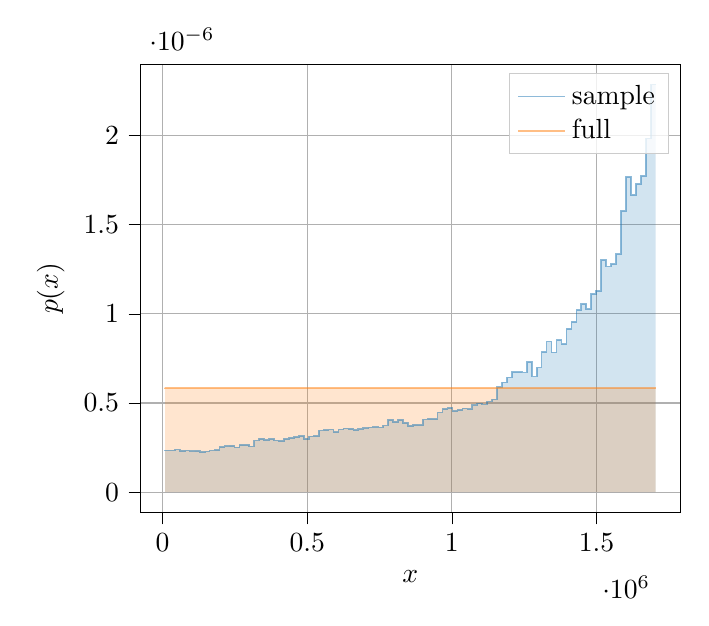
\begin{tikzpicture}

\definecolor{color0}{rgb}{0.12156862745098,0.466666666666667,0.705882352941177}
\definecolor{color1}{rgb}{1,0.498039215686275,0.0549019607843137}

\begin{axis}[
legend cell align={left},
legend style={
  fill opacity=0.8,
  draw opacity=1,
  text opacity=1,
  anchor=north east,
  draw=white!80!black
},
trim axis left,trim axis right,
tick align=outside,
tick pos=left,
x grid style={white!69.0196078431373!black},
xmajorgrids,
xmin=-76238.8255, xmax=1789470.8555,
xtick style={color=black},
xlabel={\(\displaystyle x\)},
ylabel={\(\displaystyle p(x)\)},
y grid style={white!69.0196078431373!black},
ymajorgrids,
ymin=-1.14273406088522e-07, ymax=2.39974152785897e-06,
ytick style={color=black},
ylabel near ticks
]
\path [fill=color0, fill opacity=0.2]
(axis cs:8572.13,0)
--(axis cs:8572.13,2.3099302146036e-07)
--(axis cs:8572.13,2.34399998178064e-07)
--(axis cs:25704.39,2.34399998178064e-07)
--(axis cs:25704.39,2.3433185864371e-07)
--(axis cs:42836.65,2.3433185864371e-07)
--(axis cs:42836.65,2.38897207445434e-07)
--(axis cs:59968.91,2.38897207445434e-07)
--(axis cs:59968.91,2.32355812147442e-07)
--(axis cs:77101.17,2.32355812147442e-07)
--(axis cs:77101.17,2.3399116097194e-07)
--(axis cs:94233.43,2.3399116097194e-07)
--(axis cs:94233.43,2.29016974964092e-07)
--(axis cs:111365.69,2.29016974964092e-07)
--(axis cs:111365.69,2.31129300529068e-07)
--(axis cs:128497.95,2.31129300529068e-07)
--(axis cs:128497.95,2.24383486628013e-07)
--(axis cs:145630.21,2.24383486628013e-07)
--(axis cs:145630.21,2.28403719154905e-07)
--(axis cs:162762.47,2.28403719154905e-07)
--(axis cs:162762.47,2.32900928422274e-07)
--(axis cs:179894.73,2.32900928422274e-07)
--(axis cs:179894.73,2.35217672590313e-07)
--(axis cs:197026.99,2.35217672590313e-07)
--(axis cs:197026.99,2.51911858507065e-07)
--(axis cs:214159.25,2.51911858507065e-07)
--(axis cs:214159.25,2.57090463117976e-07)
--(axis cs:231291.51,2.57090463117976e-07)
--(axis cs:231291.51,2.60361160766972e-07)
--(axis cs:248423.77,2.60361160766972e-07)
--(axis cs:248423.77,2.51094184094816e-07)
--(axis cs:265556.03,2.51094184094816e-07)
--(axis cs:265556.03,2.6465395143128e-07)
--(axis cs:282688.29,2.6465395143128e-07)
--(axis cs:282688.29,2.64585811896925e-07)
--(axis cs:299820.55,2.64585811896925e-07)
--(axis cs:299820.55,2.56000230568311e-07)
--(axis cs:316952.81,2.56000230568311e-07)
--(axis cs:316952.81,2.88775346592627e-07)
--(axis cs:334085.07,2.88775346592627e-07)
--(axis cs:334085.07,2.99541393020573e-07)
--(axis cs:351217.33,2.99541393020573e-07)
--(axis cs:351217.33,2.93749532600475e-07)
--(axis cs:368349.59,2.93749532600475e-07)
--(axis cs:368349.59,2.98178602333491e-07)
--(axis cs:385481.85,2.98178602333491e-07)
--(axis cs:385481.85,2.8966116053923e-07)
--(axis cs:402614.11,2.8966116053923e-07)
--(axis cs:402614.11,2.87889532646025e-07)
--(axis cs:419746.37,2.87889532646025e-07)
--(axis cs:419746.37,2.98042323264783e-07)
--(axis cs:436878.63,2.98042323264783e-07)
--(axis cs:436878.63,3.04924416234546e-07)
--(axis cs:454010.89,3.04924416234546e-07)
--(axis cs:454010.89,3.08263253417896e-07)
--(axis cs:471143.15,3.08263253417896e-07)
--(axis cs:471143.15,3.1466836964718e-07)
--(axis cs:488275.41,3.1466836964718e-07)
--(axis cs:488275.41,2.9981395115799e-07)
--(axis cs:505407.67,2.9981395115799e-07)
--(axis cs:505407.67,3.12147206876079e-07)
--(axis cs:522539.93,3.12147206876079e-07)
--(axis cs:522539.93,3.14804648715889e-07)
--(axis cs:539672.19,3.14804648715889e-07)
--(axis cs:539672.19,3.44854183366042e-07)
--(axis cs:556804.45,3.44854183366042e-07)
--(axis cs:556804.45,3.47852322877622e-07)
--(axis cs:573936.71,3.47852322877622e-07)
--(axis cs:573936.71,3.51123020526618e-07)
--(axis cs:591068.97,3.51123020526618e-07)
--(axis cs:591068.97,3.37086276449676e-07)
--(axis cs:608201.23,3.37086276449676e-07)
--(axis cs:608201.23,3.50646043786139e-07)
--(axis cs:625333.49,3.50646043786139e-07)
--(axis cs:625333.49,3.57187439084134e-07)
--(axis cs:642465.75,3.57187439084134e-07)
--(axis cs:642465.75,3.55483950725279e-07)
--(axis cs:659598.01,3.55483950725279e-07)
--(axis cs:659598.01,3.48056741480684e-07)
--(axis cs:676730.27,3.48056741480684e-07)
--(axis cs:676730.27,3.52349532144991e-07)
--(axis cs:693862.53,3.52349532144991e-07)
--(axis cs:693862.53,3.57936973962027e-07)
--(axis cs:710994.79,3.57936973962027e-07)
--(axis cs:710994.79,3.63183718107291e-07)
--(axis cs:728127.05,3.63183718107291e-07)
--(axis cs:728127.05,3.63456276244708e-07)
--(axis cs:745259.31,3.63456276244708e-07)
--(axis cs:745259.31,3.63047439038583e-07)
--(axis cs:762391.57,3.63047439038583e-07)
--(axis cs:762391.57,3.73677206397821e-07)
--(axis cs:779523.83,3.73677206397821e-07)
--(axis cs:779523.83,4.04612554994577e-07)
--(axis cs:796656.09,4.04612554994577e-07)
--(axis cs:796656.09,3.94868601581943e-07)
--(axis cs:813788.35,3.94868601581943e-07)
--(axis cs:813788.35,4.05293950338121e-07)
--(axis cs:830920.61,4.05293950338121e-07)
--(axis cs:830920.61,3.89281159764907e-07)
--(axis cs:848052.87,3.89281159764907e-07)
--(axis cs:848052.87,3.72314415710739e-07)
--(axis cs:865185.13,3.72314415710739e-07)
--(axis cs:865185.13,3.77424880787296e-07)
--(axis cs:882317.39,3.77424880787296e-07)
--(axis cs:882317.39,3.75108136619257e-07)
--(axis cs:899449.65,3.75108136619257e-07)
--(axis cs:899449.65,4.07269996834387e-07)
--(axis cs:916581.91,4.07269996834387e-07)
--(axis cs:916581.91,4.10404415414675e-07)
--(axis cs:933714.17,4.10404415414675e-07)
--(axis cs:933714.17,4.08837206124531e-07)
--(axis cs:950846.43,4.08837206124531e-07)
--(axis cs:950846.43,4.45905112813155e-07)
--(axis cs:967978.69,4.45905112813155e-07)
--(axis cs:967978.69,4.6716464753163e-07)
--(axis cs:985110.95,4.6716464753163e-07)
--(axis cs:985110.95,4.71048600989817e-07)
--(axis cs:1002243.21,4.71048600989817e-07)
--(axis cs:1002243.21,4.5564906622579e-07)
--(axis cs:1019375.47,4.5564906622579e-07)
--(axis cs:1019375.47,4.61304647577179e-07)
--(axis cs:1036507.73,4.61304647577179e-07)
--(axis cs:1036507.73,4.69685810302732e-07)
--(axis cs:1053639.99,4.69685810302732e-07)
--(axis cs:1053639.99,4.64847903363591e-07)
--(axis cs:1070772.25,4.64847903363591e-07)
--(axis cs:1070772.25,4.87061391563024e-07)
--(axis cs:1087904.51,4.87061391563024e-07)
--(axis cs:1087904.51,4.96737205441305e-07)
--(axis cs:1105036.77,4.96737205441305e-07)
--(axis cs:1105036.77,4.90877205486853e-07)
--(axis cs:1122169.03,4.90877205486853e-07)
--(axis cs:1122169.03,5.07707670472313e-07)
--(axis cs:1139301.29,5.07707670472313e-07)
--(axis cs:1139301.29,5.20245344793465e-07)
--(axis cs:1156433.55,5.20245344793465e-07)
--(axis cs:1156433.55,5.89747669834636e-07)
--(axis cs:1173565.81,5.89747669834636e-07)
--(axis cs:1173565.81,6.14891158011294e-07)
--(axis cs:1190698.07,6.14891158011294e-07)
--(axis cs:1190698.07,6.42896506630825e-07)
--(axis cs:1207830.33,6.42896506630825e-07)
--(axis cs:1207830.33,6.73082320349686e-07)
--(axis cs:1224962.59,6.73082320349686e-07)
--(axis cs:1224962.59,6.72809762212269e-07)
--(axis cs:1242094.85,6.72809762212269e-07)
--(axis cs:1242094.85,6.70356738975522e-07)
--(axis cs:1259227.11,6.70356738975522e-07)
--(axis cs:1259227.11,7.31137203619379e-07)
--(axis cs:1276359.37,7.31137203619379e-07)
--(axis cs:1276359.37,6.47938832173027e-07)
--(axis cs:1293491.63,6.47938832173027e-07)
--(axis cs:1293491.63,6.98293948060698e-07)
--(axis cs:1310623.89,6.98293948060698e-07)
--(axis cs:1310623.89,7.87011621789722e-07)
--(axis cs:1327756.15,7.87011621789722e-07)
--(axis cs:1327756.15,8.44657667853281e-07)
--(axis cs:1344888.41,8.44657667853281e-07)
--(axis cs:1344888.41,7.83536505537663e-07)
--(axis cs:1362020.67,7.83536505537663e-07)
--(axis cs:1362020.67,8.52084877097876e-07)
--(axis cs:1379152.93,8.52084877097876e-07)
--(axis cs:1379152.93,8.29735109829735e-07)
--(axis cs:1396285.19,8.29735109829735e-07)
--(axis cs:1396285.19,9.16408597528136e-07)
--(axis cs:1413417.45,9.16408597528136e-07)
--(axis cs:1413417.45,9.55588829781736e-07)
--(axis cs:1430549.71,9.55588829781736e-07)
--(axis cs:1430549.71,1.02236557344874e-06)
--(axis cs:1447681.97,1.02236557344874e-06)
--(axis cs:1447681.97,1.05527696854177e-06)
--(axis cs:1464814.23,1.05527696854177e-06)
--(axis cs:1464814.23,1.02590882923516e-06)
--(axis cs:1481946.49,1.02590882923516e-06)
--(axis cs:1481946.49,1.11121952624647e-06)
--(axis cs:1499078.75,1.11121952624647e-06)
--(axis cs:1499078.75,1.12879952610983e-06)
--(axis cs:1516211.01,1.12879952610983e-06)
--(axis cs:1516211.01,1.30221464104098e-06)
--(axis cs:1533343.27,1.30221464104098e-06)
--(axis cs:1533343.27,1.26501045528365e-06)
--(axis cs:1550475.53,1.26501045528365e-06)
--(axis cs:1550475.53,1.27816138541399e-06)
--(axis cs:1567607.79,1.27816138541399e-06)
--(axis cs:1567607.79,1.33417208265305e-06)
--(axis cs:1584740.05,1.33417208265305e-06)
--(axis cs:1584740.05,1.57736208076279e-06)
--(axis cs:1601872.31,1.57736208076279e-06)
--(axis cs:1601872.31,1.76801649788553e-06)
--(axis cs:1619004.57,1.76801649788553e-06)
--(axis cs:1619004.57,1.66682928936971e-06)
--(axis cs:1636136.83,1.66682928936971e-06)
--(axis cs:1636136.83,1.72897254470066e-06)
--(axis cs:1653269.09,1.72897254470066e-06)
--(axis cs:1653269.09,1.77387649783998e-06)
--(axis cs:1670401.35,1.77387649783998e-06)
--(axis cs:1670401.35,1.98381440318493e-06)
--(axis cs:1687533.61,1.98381440318493e-06)
--(axis cs:1687533.61,2.28546812177045e-06)
--(axis cs:1704665.87,2.28546812177045e-06)
--(axis cs:1704665.87,0)
--(axis cs:1704665.87,0)
--(axis cs:1687533.61,0)
--(axis cs:1687533.61,0)
--(axis cs:1670401.35,0)
--(axis cs:1670401.35,0)
--(axis cs:1653269.09,0)
--(axis cs:1653269.09,0)
--(axis cs:1636136.83,0)
--(axis cs:1636136.83,0)
--(axis cs:1619004.57,0)
--(axis cs:1619004.57,0)
--(axis cs:1601872.31,0)
--(axis cs:1601872.31,0)
--(axis cs:1584740.05,0)
--(axis cs:1584740.05,0)
--(axis cs:1567607.79,0)
--(axis cs:1567607.79,0)
--(axis cs:1550475.53,0)
--(axis cs:1550475.53,0)
--(axis cs:1533343.27,0)
--(axis cs:1533343.27,0)
--(axis cs:1516211.01,0)
--(axis cs:1516211.01,0)
--(axis cs:1499078.75,0)
--(axis cs:1499078.75,0)
--(axis cs:1481946.49,0)
--(axis cs:1481946.49,0)
--(axis cs:1464814.23,0)
--(axis cs:1464814.23,0)
--(axis cs:1447681.97,0)
--(axis cs:1447681.97,0)
--(axis cs:1430549.71,0)
--(axis cs:1430549.71,0)
--(axis cs:1413417.45,0)
--(axis cs:1413417.45,0)
--(axis cs:1396285.19,0)
--(axis cs:1396285.19,0)
--(axis cs:1379152.93,0)
--(axis cs:1379152.93,0)
--(axis cs:1362020.67,0)
--(axis cs:1362020.67,0)
--(axis cs:1344888.41,0)
--(axis cs:1344888.41,0)
--(axis cs:1327756.15,0)
--(axis cs:1327756.15,0)
--(axis cs:1310623.89,0)
--(axis cs:1310623.89,0)
--(axis cs:1293491.63,0)
--(axis cs:1293491.63,0)
--(axis cs:1276359.37,0)
--(axis cs:1276359.37,0)
--(axis cs:1259227.11,0)
--(axis cs:1259227.11,0)
--(axis cs:1242094.85,0)
--(axis cs:1242094.85,0)
--(axis cs:1224962.59,0)
--(axis cs:1224962.59,0)
--(axis cs:1207830.33,0)
--(axis cs:1207830.33,0)
--(axis cs:1190698.07,0)
--(axis cs:1190698.07,0)
--(axis cs:1173565.81,0)
--(axis cs:1173565.81,0)
--(axis cs:1156433.55,0)
--(axis cs:1156433.55,0)
--(axis cs:1139301.29,0)
--(axis cs:1139301.29,0)
--(axis cs:1122169.03,0)
--(axis cs:1122169.03,0)
--(axis cs:1105036.77,0)
--(axis cs:1105036.77,0)
--(axis cs:1087904.51,0)
--(axis cs:1087904.51,0)
--(axis cs:1070772.25,0)
--(axis cs:1070772.25,0)
--(axis cs:1053639.99,0)
--(axis cs:1053639.99,0)
--(axis cs:1036507.73,0)
--(axis cs:1036507.73,0)
--(axis cs:1019375.47,0)
--(axis cs:1019375.47,0)
--(axis cs:1002243.21,0)
--(axis cs:1002243.21,0)
--(axis cs:985110.95,0)
--(axis cs:985110.95,0)
--(axis cs:967978.69,0)
--(axis cs:967978.69,0)
--(axis cs:950846.43,0)
--(axis cs:950846.43,0)
--(axis cs:933714.17,0)
--(axis cs:933714.17,0)
--(axis cs:916581.91,0)
--(axis cs:916581.91,0)
--(axis cs:899449.65,0)
--(axis cs:899449.65,0)
--(axis cs:882317.39,0)
--(axis cs:882317.39,0)
--(axis cs:865185.13,0)
--(axis cs:865185.13,0)
--(axis cs:848052.87,0)
--(axis cs:848052.87,0)
--(axis cs:830920.61,0)
--(axis cs:830920.61,0)
--(axis cs:813788.35,0)
--(axis cs:813788.35,0)
--(axis cs:796656.09,0)
--(axis cs:796656.09,0)
--(axis cs:779523.83,0)
--(axis cs:779523.83,0)
--(axis cs:762391.57,0)
--(axis cs:762391.57,0)
--(axis cs:745259.31,0)
--(axis cs:745259.31,0)
--(axis cs:728127.05,0)
--(axis cs:728127.05,0)
--(axis cs:710994.79,0)
--(axis cs:710994.79,0)
--(axis cs:693862.53,0)
--(axis cs:693862.53,0)
--(axis cs:676730.27,0)
--(axis cs:676730.27,0)
--(axis cs:659598.01,0)
--(axis cs:659598.01,0)
--(axis cs:642465.75,0)
--(axis cs:642465.75,0)
--(axis cs:625333.49,0)
--(axis cs:625333.49,0)
--(axis cs:608201.23,0)
--(axis cs:608201.23,0)
--(axis cs:591068.97,0)
--(axis cs:591068.97,0)
--(axis cs:573936.71,0)
--(axis cs:573936.71,0)
--(axis cs:556804.45,0)
--(axis cs:556804.45,0)
--(axis cs:539672.19,0)
--(axis cs:539672.19,0)
--(axis cs:522539.93,0)
--(axis cs:522539.93,0)
--(axis cs:505407.67,0)
--(axis cs:505407.67,0)
--(axis cs:488275.41,0)
--(axis cs:488275.41,0)
--(axis cs:471143.15,0)
--(axis cs:471143.15,0)
--(axis cs:454010.89,0)
--(axis cs:454010.89,0)
--(axis cs:436878.63,0)
--(axis cs:436878.63,0)
--(axis cs:419746.37,0)
--(axis cs:419746.37,0)
--(axis cs:402614.11,0)
--(axis cs:402614.11,0)
--(axis cs:385481.85,0)
--(axis cs:385481.85,0)
--(axis cs:368349.59,0)
--(axis cs:368349.59,0)
--(axis cs:351217.33,0)
--(axis cs:351217.33,0)
--(axis cs:334085.07,0)
--(axis cs:334085.07,0)
--(axis cs:316952.81,0)
--(axis cs:316952.81,0)
--(axis cs:299820.55,0)
--(axis cs:299820.55,0)
--(axis cs:282688.29,0)
--(axis cs:282688.29,0)
--(axis cs:265556.03,0)
--(axis cs:265556.03,0)
--(axis cs:248423.77,0)
--(axis cs:248423.77,0)
--(axis cs:231291.51,0)
--(axis cs:231291.51,0)
--(axis cs:214159.25,0)
--(axis cs:214159.25,0)
--(axis cs:197026.99,0)
--(axis cs:197026.99,0)
--(axis cs:179894.73,0)
--(axis cs:179894.73,0)
--(axis cs:162762.47,0)
--(axis cs:162762.47,0)
--(axis cs:145630.21,0)
--(axis cs:145630.21,0)
--(axis cs:128497.95,0)
--(axis cs:128497.95,0)
--(axis cs:111365.69,0)
--(axis cs:111365.69,0)
--(axis cs:94233.43,0)
--(axis cs:94233.43,0)
--(axis cs:77101.17,0)
--(axis cs:77101.17,0)
--(axis cs:59968.91,0)
--(axis cs:59968.91,0)
--(axis cs:42836.65,0)
--(axis cs:42836.65,0)
--(axis cs:25704.39,0)
--(axis cs:25704.39,0)
--(axis cs:8572.13,0)
--(axis cs:8572.13,0)
--cycle;

\path [fill=color1, fill opacity=0.2]
(axis cs:8566.16,0)
--(axis cs:8566.16,5.8371493606733e-07)
--(axis cs:8566.16,5.83680866439357e-07)
--(axis cs:25698.48,5.83680866439357e-07)
--(axis cs:25698.48,5.83680866439357e-07)
--(axis cs:42830.8,5.83680866439357e-07)
--(axis cs:42830.8,5.8371493606733e-07)
--(axis cs:59963.12,5.8371493606733e-07)
--(axis cs:59963.12,5.83680866439357e-07)
--(axis cs:77095.44,5.83680866439357e-07)
--(axis cs:77095.44,5.83680866439357e-07)
--(axis cs:94227.76,5.83680866439357e-07)
--(axis cs:94227.76,5.83714936067331e-07)
--(axis cs:111360.08,5.83714936067331e-07)
--(axis cs:111360.08,5.83680866439357e-07)
--(axis cs:128492.4,5.83680866439357e-07)
--(axis cs:128492.4,5.83680866439357e-07)
--(axis cs:145624.72,5.83680866439357e-07)
--(axis cs:145624.72,5.8371493606733e-07)
--(axis cs:162757.04,5.8371493606733e-07)
--(axis cs:162757.04,5.83680866439358e-07)
--(axis cs:179889.36,5.83680866439358e-07)
--(axis cs:179889.36,5.83680866439357e-07)
--(axis cs:197021.68,5.83680866439357e-07)
--(axis cs:197021.68,5.8371493606733e-07)
--(axis cs:214154,5.8371493606733e-07)
--(axis cs:214154,5.83680866439358e-07)
--(axis cs:231286.32,5.83680866439358e-07)
--(axis cs:231286.32,5.83680866439357e-07)
--(axis cs:248418.64,5.83680866439357e-07)
--(axis cs:248418.64,5.8371493606733e-07)
--(axis cs:265550.96,5.8371493606733e-07)
--(axis cs:265550.96,5.83680866439357e-07)
--(axis cs:282683.28,5.83680866439357e-07)
--(axis cs:282683.28,5.83680866439357e-07)
--(axis cs:299815.6,5.83680866439357e-07)
--(axis cs:299815.6,5.8371493606733e-07)
--(axis cs:316947.92,5.8371493606733e-07)
--(axis cs:316947.92,5.83680866439357e-07)
--(axis cs:334080.24,5.83680866439357e-07)
--(axis cs:334080.24,5.83680866439359e-07)
--(axis cs:351212.56,5.83680866439359e-07)
--(axis cs:351212.56,5.8371493606733e-07)
--(axis cs:368344.88,5.8371493606733e-07)
--(axis cs:368344.88,5.83680866439357e-07)
--(axis cs:385477.2,5.83680866439357e-07)
--(axis cs:385477.2,5.83680866439357e-07)
--(axis cs:402609.52,5.83680866439357e-07)
--(axis cs:402609.52,5.83680866439357e-07)
--(axis cs:419741.84,5.83680866439357e-07)
--(axis cs:419741.84,5.8371493606733e-07)
--(axis cs:436874.16,5.8371493606733e-07)
--(axis cs:436874.16,5.83680866439357e-07)
--(axis cs:454006.48,5.83680866439357e-07)
--(axis cs:454006.48,5.83680866439359e-07)
--(axis cs:471138.8,5.83680866439359e-07)
--(axis cs:471138.8,5.8371493606733e-07)
--(axis cs:488271.12,5.8371493606733e-07)
--(axis cs:488271.12,5.83680866439357e-07)
--(axis cs:505403.44,5.83680866439357e-07)
--(axis cs:505403.44,5.83680866439355e-07)
--(axis cs:522535.76,5.83680866439355e-07)
--(axis cs:522535.76,5.83714936067332e-07)
--(axis cs:539668.08,5.83714936067332e-07)
--(axis cs:539668.08,5.83680866439359e-07)
--(axis cs:556800.4,5.83680866439359e-07)
--(axis cs:556800.4,5.83680866439355e-07)
--(axis cs:573932.72,5.83680866439355e-07)
--(axis cs:573932.72,5.83714936067332e-07)
--(axis cs:591065.04,5.83714936067332e-07)
--(axis cs:591065.04,5.83680866439355e-07)
--(axis cs:608197.36,5.83680866439355e-07)
--(axis cs:608197.36,5.83680866439359e-07)
--(axis cs:625329.68,5.83680866439359e-07)
--(axis cs:625329.68,5.83714936067328e-07)
--(axis cs:642462,5.83714936067328e-07)
--(axis cs:642462,5.83680866439359e-07)
--(axis cs:659594.32,5.83680866439359e-07)
--(axis cs:659594.32,5.83680866439355e-07)
--(axis cs:676726.64,5.83680866439355e-07)
--(axis cs:676726.64,5.83714936067332e-07)
--(axis cs:693858.96,5.83714936067332e-07)
--(axis cs:693858.96,5.83680866439359e-07)
--(axis cs:710991.28,5.83680866439359e-07)
--(axis cs:710991.28,5.83680866439355e-07)
--(axis cs:728123.6,5.83680866439355e-07)
--(axis cs:728123.6,5.83714936067332e-07)
--(axis cs:745255.92,5.83714936067332e-07)
--(axis cs:745255.92,5.83680866439355e-07)
--(axis cs:762388.24,5.83680866439355e-07)
--(axis cs:762388.24,5.83680866439359e-07)
--(axis cs:779520.56,5.83680866439359e-07)
--(axis cs:779520.56,5.83714936067328e-07)
--(axis cs:796652.88,5.83714936067328e-07)
--(axis cs:796652.88,5.83680866439359e-07)
--(axis cs:813785.2,5.83680866439359e-07)
--(axis cs:813785.2,5.83680866439359e-07)
--(axis cs:830917.52,5.83680866439359e-07)
--(axis cs:830917.52,5.83680866439355e-07)
--(axis cs:848049.84,5.83680866439355e-07)
--(axis cs:848049.84,5.83714936067332e-07)
--(axis cs:865182.16,5.83714936067332e-07)
--(axis cs:865182.16,5.83680866439355e-07)
--(axis cs:882314.48,5.83680866439355e-07)
--(axis cs:882314.48,5.83680866439359e-07)
--(axis cs:899446.8,5.83680866439359e-07)
--(axis cs:899446.8,5.83714936067328e-07)
--(axis cs:916579.12,5.83714936067328e-07)
--(axis cs:916579.12,5.83680866439359e-07)
--(axis cs:933711.44,5.83680866439359e-07)
--(axis cs:933711.44,5.83680866439359e-07)
--(axis cs:950843.76,5.83680866439359e-07)
--(axis cs:950843.76,5.83714936067328e-07)
--(axis cs:967976.08,5.83714936067328e-07)
--(axis cs:967976.08,5.83680866439359e-07)
--(axis cs:985108.4,5.83680866439359e-07)
--(axis cs:985108.4,5.83680866439355e-07)
--(axis cs:1002240.72,5.83680866439355e-07)
--(axis cs:1002240.72,5.83714936067332e-07)
--(axis cs:1019373.04,5.83714936067332e-07)
--(axis cs:1019373.04,5.83680866439355e-07)
--(axis cs:1036505.36,5.83680866439355e-07)
--(axis cs:1036505.36,5.83680866439355e-07)
--(axis cs:1053637.68,5.83680866439355e-07)
--(axis cs:1053637.68,5.83714936067336e-07)
--(axis cs:1070770,5.83714936067336e-07)
--(axis cs:1070770,5.83680866439355e-07)
--(axis cs:1087902.32,5.83680866439355e-07)
--(axis cs:1087902.32,5.83680866439355e-07)
--(axis cs:1105034.64,5.83680866439355e-07)
--(axis cs:1105034.64,5.83714936067336e-07)
--(axis cs:1122166.96,5.83714936067336e-07)
--(axis cs:1122166.96,5.83680866439355e-07)
--(axis cs:1139299.28,5.83680866439355e-07)
--(axis cs:1139299.28,5.83680866439355e-07)
--(axis cs:1156431.6,5.83680866439355e-07)
--(axis cs:1156431.6,5.83714936067328e-07)
--(axis cs:1173563.92,5.83714936067328e-07)
--(axis cs:1173563.92,5.83680866439363e-07)
--(axis cs:1190696.24,5.83680866439363e-07)
--(axis cs:1190696.24,5.83680866439355e-07)
--(axis cs:1207828.56,5.83680866439355e-07)
--(axis cs:1207828.56,5.83714936067328e-07)
--(axis cs:1224960.88,5.83714936067328e-07)
--(axis cs:1224960.88,5.83680866439363e-07)
--(axis cs:1242093.2,5.83680866439363e-07)
--(axis cs:1242093.2,5.83680866439355e-07)
--(axis cs:1259225.52,5.83680866439355e-07)
--(axis cs:1259225.52,5.83680866439355e-07)
--(axis cs:1276357.84,5.83680866439355e-07)
--(axis cs:1276357.84,5.83714936067328e-07)
--(axis cs:1293490.16,5.83714936067328e-07)
--(axis cs:1293490.16,5.83680866439363e-07)
--(axis cs:1310622.48,5.83680866439363e-07)
--(axis cs:1310622.48,5.83680866439355e-07)
--(axis cs:1327754.8,5.83680866439355e-07)
--(axis cs:1327754.8,5.83714936067328e-07)
--(axis cs:1344887.12,5.83714936067328e-07)
--(axis cs:1344887.12,5.83680866439355e-07)
--(axis cs:1362019.44,5.83680866439355e-07)
--(axis cs:1362019.44,5.83680866439363e-07)
--(axis cs:1379151.76,5.83680866439363e-07)
--(axis cs:1379151.76,5.83714936067328e-07)
--(axis cs:1396284.08,5.83714936067328e-07)
--(axis cs:1396284.08,5.83680866439355e-07)
--(axis cs:1413416.4,5.83680866439355e-07)
--(axis cs:1413416.4,5.83680866439363e-07)
--(axis cs:1430548.72,5.83680866439363e-07)
--(axis cs:1430548.72,5.83714936067328e-07)
--(axis cs:1447681.04,5.83714936067328e-07)
--(axis cs:1447681.04,5.83680866439355e-07)
--(axis cs:1464813.36,5.83680866439355e-07)
--(axis cs:1464813.36,5.83680866439355e-07)
--(axis cs:1481945.68,5.83680866439355e-07)
--(axis cs:1481945.68,5.83714936067336e-07)
--(axis cs:1499078,5.83714936067336e-07)
--(axis cs:1499078,5.83680866439355e-07)
--(axis cs:1516210.32,5.83680866439355e-07)
--(axis cs:1516210.32,5.83680866439355e-07)
--(axis cs:1533342.64,5.83680866439355e-07)
--(axis cs:1533342.64,5.83714936067336e-07)
--(axis cs:1550474.96,5.83714936067336e-07)
--(axis cs:1550474.96,5.83680866439355e-07)
--(axis cs:1567607.28,5.83680866439355e-07)
--(axis cs:1567607.28,5.83680866439355e-07)
--(axis cs:1584739.6,5.83680866439355e-07)
--(axis cs:1584739.6,5.83714936067328e-07)
--(axis cs:1601871.92,5.83714936067328e-07)
--(axis cs:1601871.92,5.83680866439363e-07)
--(axis cs:1619004.24,5.83680866439363e-07)
--(axis cs:1619004.24,5.83680866439355e-07)
--(axis cs:1636136.56,5.83680866439355e-07)
--(axis cs:1636136.56,5.83714936067328e-07)
--(axis cs:1653268.88,5.83714936067328e-07)
--(axis cs:1653268.88,5.83680866439363e-07)
--(axis cs:1670401.2,5.83680866439363e-07)
--(axis cs:1670401.2,5.83680866439355e-07)
--(axis cs:1687533.52,5.83680866439355e-07)
--(axis cs:1687533.52,5.83714936067328e-07)
--(axis cs:1704665.84,5.83714936067328e-07)
--(axis cs:1704665.84,0)
--(axis cs:1704665.84,0)
--(axis cs:1687533.52,0)
--(axis cs:1687533.52,0)
--(axis cs:1670401.2,0)
--(axis cs:1670401.2,0)
--(axis cs:1653268.88,0)
--(axis cs:1653268.88,0)
--(axis cs:1636136.56,0)
--(axis cs:1636136.56,0)
--(axis cs:1619004.24,0)
--(axis cs:1619004.24,0)
--(axis cs:1601871.92,0)
--(axis cs:1601871.92,0)
--(axis cs:1584739.6,0)
--(axis cs:1584739.6,0)
--(axis cs:1567607.28,0)
--(axis cs:1567607.28,0)
--(axis cs:1550474.96,0)
--(axis cs:1550474.96,0)
--(axis cs:1533342.64,0)
--(axis cs:1533342.64,0)
--(axis cs:1516210.32,0)
--(axis cs:1516210.32,0)
--(axis cs:1499078,0)
--(axis cs:1499078,0)
--(axis cs:1481945.68,0)
--(axis cs:1481945.68,0)
--(axis cs:1464813.36,0)
--(axis cs:1464813.36,0)
--(axis cs:1447681.04,0)
--(axis cs:1447681.04,0)
--(axis cs:1430548.72,0)
--(axis cs:1430548.72,0)
--(axis cs:1413416.4,0)
--(axis cs:1413416.4,0)
--(axis cs:1396284.08,0)
--(axis cs:1396284.08,0)
--(axis cs:1379151.76,0)
--(axis cs:1379151.76,0)
--(axis cs:1362019.44,0)
--(axis cs:1362019.44,0)
--(axis cs:1344887.12,0)
--(axis cs:1344887.12,0)
--(axis cs:1327754.8,0)
--(axis cs:1327754.8,0)
--(axis cs:1310622.48,0)
--(axis cs:1310622.48,0)
--(axis cs:1293490.16,0)
--(axis cs:1293490.16,0)
--(axis cs:1276357.84,0)
--(axis cs:1276357.84,0)
--(axis cs:1259225.52,0)
--(axis cs:1259225.52,0)
--(axis cs:1242093.2,0)
--(axis cs:1242093.2,0)
--(axis cs:1224960.88,0)
--(axis cs:1224960.88,0)
--(axis cs:1207828.56,0)
--(axis cs:1207828.56,0)
--(axis cs:1190696.24,0)
--(axis cs:1190696.24,0)
--(axis cs:1173563.92,0)
--(axis cs:1173563.92,0)
--(axis cs:1156431.6,0)
--(axis cs:1156431.6,0)
--(axis cs:1139299.28,0)
--(axis cs:1139299.28,0)
--(axis cs:1122166.96,0)
--(axis cs:1122166.96,0)
--(axis cs:1105034.64,0)
--(axis cs:1105034.64,0)
--(axis cs:1087902.32,0)
--(axis cs:1087902.32,0)
--(axis cs:1070770,0)
--(axis cs:1070770,0)
--(axis cs:1053637.68,0)
--(axis cs:1053637.68,0)
--(axis cs:1036505.36,0)
--(axis cs:1036505.36,0)
--(axis cs:1019373.04,0)
--(axis cs:1019373.04,0)
--(axis cs:1002240.72,0)
--(axis cs:1002240.72,0)
--(axis cs:985108.4,0)
--(axis cs:985108.4,0)
--(axis cs:967976.08,0)
--(axis cs:967976.08,0)
--(axis cs:950843.76,0)
--(axis cs:950843.76,0)
--(axis cs:933711.44,0)
--(axis cs:933711.44,0)
--(axis cs:916579.12,0)
--(axis cs:916579.12,0)
--(axis cs:899446.8,0)
--(axis cs:899446.8,0)
--(axis cs:882314.48,0)
--(axis cs:882314.48,0)
--(axis cs:865182.16,0)
--(axis cs:865182.16,0)
--(axis cs:848049.84,0)
--(axis cs:848049.84,0)
--(axis cs:830917.52,0)
--(axis cs:830917.52,0)
--(axis cs:813785.2,0)
--(axis cs:813785.2,0)
--(axis cs:796652.88,0)
--(axis cs:796652.88,0)
--(axis cs:779520.56,0)
--(axis cs:779520.56,0)
--(axis cs:762388.24,0)
--(axis cs:762388.24,0)
--(axis cs:745255.92,0)
--(axis cs:745255.92,0)
--(axis cs:728123.6,0)
--(axis cs:728123.6,0)
--(axis cs:710991.28,0)
--(axis cs:710991.28,0)
--(axis cs:693858.96,0)
--(axis cs:693858.96,0)
--(axis cs:676726.64,0)
--(axis cs:676726.64,0)
--(axis cs:659594.32,0)
--(axis cs:659594.32,0)
--(axis cs:642462,0)
--(axis cs:642462,0)
--(axis cs:625329.68,0)
--(axis cs:625329.68,0)
--(axis cs:608197.36,0)
--(axis cs:608197.36,0)
--(axis cs:591065.04,0)
--(axis cs:591065.04,0)
--(axis cs:573932.72,0)
--(axis cs:573932.72,0)
--(axis cs:556800.4,0)
--(axis cs:556800.4,0)
--(axis cs:539668.08,0)
--(axis cs:539668.08,0)
--(axis cs:522535.76,0)
--(axis cs:522535.76,0)
--(axis cs:505403.44,0)
--(axis cs:505403.44,0)
--(axis cs:488271.12,0)
--(axis cs:488271.12,0)
--(axis cs:471138.8,0)
--(axis cs:471138.8,0)
--(axis cs:454006.48,0)
--(axis cs:454006.48,0)
--(axis cs:436874.16,0)
--(axis cs:436874.16,0)
--(axis cs:419741.84,0)
--(axis cs:419741.84,0)
--(axis cs:402609.52,0)
--(axis cs:402609.52,0)
--(axis cs:385477.2,0)
--(axis cs:385477.2,0)
--(axis cs:368344.88,0)
--(axis cs:368344.88,0)
--(axis cs:351212.56,0)
--(axis cs:351212.56,0)
--(axis cs:334080.24,0)
--(axis cs:334080.24,0)
--(axis cs:316947.92,0)
--(axis cs:316947.92,0)
--(axis cs:299815.6,0)
--(axis cs:299815.6,0)
--(axis cs:282683.28,0)
--(axis cs:282683.28,0)
--(axis cs:265550.96,0)
--(axis cs:265550.96,0)
--(axis cs:248418.64,0)
--(axis cs:248418.64,0)
--(axis cs:231286.32,0)
--(axis cs:231286.32,0)
--(axis cs:214154,0)
--(axis cs:214154,0)
--(axis cs:197021.68,0)
--(axis cs:197021.68,0)
--(axis cs:179889.36,0)
--(axis cs:179889.36,0)
--(axis cs:162757.04,0)
--(axis cs:162757.04,0)
--(axis cs:145624.72,0)
--(axis cs:145624.72,0)
--(axis cs:128492.4,0)
--(axis cs:128492.4,0)
--(axis cs:111360.08,0)
--(axis cs:111360.08,0)
--(axis cs:94227.76,0)
--(axis cs:94227.76,0)
--(axis cs:77095.44,0)
--(axis cs:77095.44,0)
--(axis cs:59963.12,0)
--(axis cs:59963.12,0)
--(axis cs:42830.8,0)
--(axis cs:42830.8,0)
--(axis cs:25698.48,0)
--(axis cs:25698.48,0)
--(axis cs:8566.16,0)
--(axis cs:8566.16,0)
--cycle;

\addplot [semithick, color0, const plot mark right, opacity=0.5]
table {%
8572.13 2.3099302146036e-07
25704.39 2.34399998178064e-07
42836.65 2.3433185864371e-07
59968.91 2.38897207445434e-07
77101.17 2.32355812147442e-07
94233.43 2.3399116097194e-07
111365.69 2.29016974964092e-07
128497.95 2.31129300529068e-07
145630.21 2.24383486628013e-07
162762.47 2.28403719154905e-07
179894.73 2.32900928422274e-07
197026.99 2.35217672590313e-07
214159.25 2.51911858507065e-07
231291.51 2.57090463117976e-07
248423.77 2.60361160766972e-07
265556.03 2.51094184094816e-07
282688.29 2.6465395143128e-07
299820.55 2.64585811896925e-07
316952.81 2.56000230568311e-07
334085.07 2.88775346592627e-07
351217.33 2.99541393020573e-07
368349.59 2.93749532600475e-07
385481.85 2.98178602333491e-07
402614.11 2.8966116053923e-07
419746.37 2.87889532646025e-07
436878.63 2.98042323264783e-07
454010.89 3.04924416234546e-07
471143.15 3.08263253417896e-07
488275.41 3.1466836964718e-07
505407.67 2.9981395115799e-07
522539.93 3.12147206876079e-07
539672.19 3.14804648715889e-07
556804.45 3.44854183366042e-07
573936.71 3.47852322877622e-07
591068.97 3.51123020526618e-07
608201.23 3.37086276449676e-07
625333.49 3.50646043786139e-07
642465.75 3.57187439084134e-07
659598.01 3.55483950725279e-07
676730.27 3.48056741480684e-07
693862.53 3.52349532144991e-07
710994.79 3.57936973962027e-07
728127.05 3.63183718107291e-07
745259.31 3.63456276244708e-07
762391.57 3.63047439038583e-07
779523.83 3.73677206397821e-07
796656.09 4.04612554994577e-07
813788.35 3.94868601581943e-07
830920.61 4.05293950338121e-07
848052.87 3.89281159764907e-07
865185.13 3.72314415710739e-07
882317.39 3.77424880787296e-07
899449.65 3.75108136619257e-07
916581.91 4.07269996834387e-07
933714.17 4.10404415414675e-07
950846.43 4.08837206124531e-07
967978.69 4.45905112813155e-07
985110.95 4.6716464753163e-07
1002243.21 4.71048600989817e-07
1019375.47 4.5564906622579e-07
1036507.73 4.61304647577179e-07
1053639.99 4.69685810302732e-07
1070772.25 4.64847903363591e-07
1087904.51 4.87061391563024e-07
1105036.77 4.96737205441305e-07
1122169.03 4.90877205486853e-07
1139301.29 5.07707670472313e-07
1156433.55 5.20245344793465e-07
1173565.81 5.89747669834636e-07
1190698.07 6.14891158011294e-07
1207830.33 6.42896506630825e-07
1224962.59 6.73082320349686e-07
1242094.85 6.72809762212269e-07
1259227.11 6.70356738975522e-07
1276359.37 7.31137203619379e-07
1293491.63 6.47938832173027e-07
1310623.89 6.98293948060698e-07
1327756.15 7.87011621789722e-07
1344888.41 8.44657667853281e-07
1362020.67 7.83536505537663e-07
1379152.93 8.52084877097876e-07
1396285.19 8.29735109829735e-07
1413417.45 9.16408597528136e-07
1430549.71 9.55588829781736e-07
1447681.97 1.02236557344874e-06
1464814.23 1.05527696854177e-06
1481946.49 1.02590882923516e-06
1499078.75 1.11121952624647e-06
1516211.01 1.12879952610983e-06
1533343.27 1.30221464104098e-06
1550475.53 1.26501045528365e-06
1567607.79 1.27816138541399e-06
1584740.05 1.33417208265305e-06
1601872.31 1.57736208076279e-06
1619004.57 1.76801649788553e-06
1636136.83 1.66682928936971e-06
1653269.09 1.72897254470066e-06
1670401.35 1.77387649783998e-06
1687533.61 1.98381440318493e-06
1704665.87 2.28546812177045e-06
};
\addlegendentry{sample}
\addplot [semithick, color1, const plot mark right, opacity=0.5]
table {%
8566.16 5.8371493606733e-07
25698.48 5.83680866439357e-07
42830.8 5.83680866439357e-07
59963.12 5.8371493606733e-07
77095.44 5.83680866439357e-07
94227.76 5.83680866439357e-07
111360.08 5.83714936067331e-07
128492.4 5.83680866439357e-07
145624.72 5.83680866439357e-07
162757.04 5.8371493606733e-07
179889.36 5.83680866439358e-07
197021.68 5.83680866439357e-07
214154 5.8371493606733e-07
231286.32 5.83680866439358e-07
248418.64 5.83680866439357e-07
265550.96 5.8371493606733e-07
282683.28 5.83680866439357e-07
299815.6 5.83680866439357e-07
316947.92 5.8371493606733e-07
334080.24 5.83680866439357e-07
351212.56 5.83680866439359e-07
368344.88 5.8371493606733e-07
385477.2 5.83680866439357e-07
402609.52 5.83680866439357e-07
419741.84 5.83680866439357e-07
436874.16 5.8371493606733e-07
454006.48 5.83680866439357e-07
471138.8 5.83680866439359e-07
488271.12 5.8371493606733e-07
505403.44 5.83680866439357e-07
522535.76 5.83680866439355e-07
539668.08 5.83714936067332e-07
556800.4 5.83680866439359e-07
573932.72 5.83680866439355e-07
591065.04 5.83714936067332e-07
608197.36 5.83680866439355e-07
625329.68 5.83680866439359e-07
642462 5.83714936067328e-07
659594.32 5.83680866439359e-07
676726.64 5.83680866439355e-07
693858.96 5.83714936067332e-07
710991.28 5.83680866439359e-07
728123.6 5.83680866439355e-07
745255.92 5.83714936067332e-07
762388.24 5.83680866439355e-07
779520.56 5.83680866439359e-07
796652.88 5.83714936067328e-07
813785.2 5.83680866439359e-07
830917.52 5.83680866439359e-07
848049.84 5.83680866439355e-07
865182.16 5.83714936067332e-07
882314.48 5.83680866439355e-07
899446.8 5.83680866439359e-07
916579.12 5.83714936067328e-07
933711.44 5.83680866439359e-07
950843.76 5.83680866439359e-07
967976.08 5.83714936067328e-07
985108.4 5.83680866439359e-07
1002240.72 5.83680866439355e-07
1019373.04 5.83714936067332e-07
1036505.36 5.83680866439355e-07
1053637.68 5.83680866439355e-07
1070770 5.83714936067336e-07
1087902.32 5.83680866439355e-07
1105034.64 5.83680866439355e-07
1122166.96 5.83714936067336e-07
1139299.28 5.83680866439355e-07
1156431.6 5.83680866439355e-07
1173563.92 5.83714936067328e-07
1190696.24 5.83680866439363e-07
1207828.56 5.83680866439355e-07
1224960.88 5.83714936067328e-07
1242093.2 5.83680866439363e-07
1259225.52 5.83680866439355e-07
1276357.84 5.83680866439355e-07
1293490.16 5.83714936067328e-07
1310622.48 5.83680866439363e-07
1327754.8 5.83680866439355e-07
1344887.12 5.83714936067328e-07
1362019.44 5.83680866439355e-07
1379151.76 5.83680866439363e-07
1396284.08 5.83714936067328e-07
1413416.4 5.83680866439355e-07
1430548.72 5.83680866439363e-07
1447681.04 5.83714936067328e-07
1464813.36 5.83680866439355e-07
1481945.68 5.83680866439355e-07
1499078 5.83714936067336e-07
1516210.32 5.83680866439355e-07
1533342.64 5.83680866439355e-07
1550474.96 5.83714936067336e-07
1567607.28 5.83680866439355e-07
1584739.6 5.83680866439355e-07
1601871.92 5.83714936067328e-07
1619004.24 5.83680866439363e-07
1636136.56 5.83680866439355e-07
1653268.88 5.83714936067328e-07
1670401.2 5.83680866439363e-07
1687533.52 5.83680866439355e-07
1704665.84 5.83714936067328e-07
};
\addlegendentry{full}
\end{axis}

\end{tikzpicture}

	\end{adjustbox}}\medskip{}
\subfloat[KS tests for $n\protect\coloneqq10^{3},10^{4}$ and $f\protect\coloneqq0.1,\dots,0.9$.\label{fig:Wander-join}]{    \centering
    \begin{adjustbox}{width=\linewidth,center}
    	% This file was created by tikzplotlib v0.9.8.
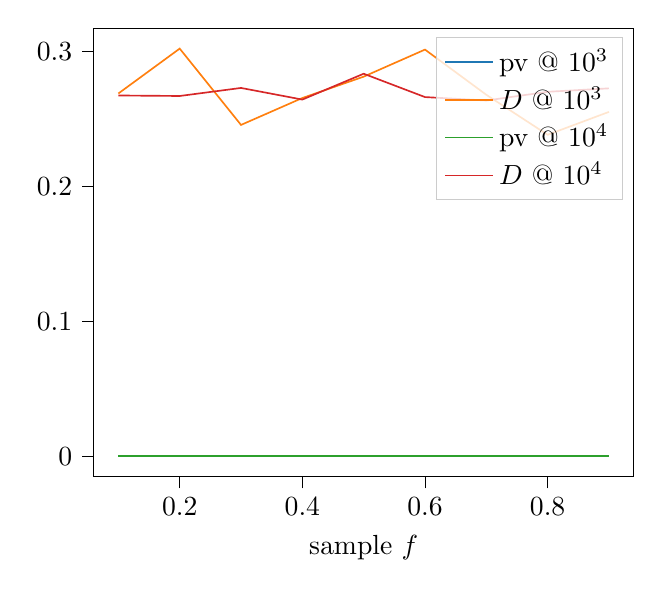
\begin{tikzpicture}

\definecolor{color0}{rgb}{0.12156862745098,0.466666666666667,0.705882352941177}
\definecolor{color1}{rgb}{1,0.498039215686275,0.0549019607843137}
\definecolor{color2}{rgb}{0.172549019607843,0.627450980392157,0.172549019607843}
\definecolor{color3}{rgb}{0.83921568627451,0.152941176470588,0.156862745098039}

\begin{axis}[
legend cell align={left},
legend style={fill opacity=0.8, draw opacity=1, text opacity=1, draw=white!80!black},
tick align=outside,
tick pos=left,
x grid style={white!69.0196078431373!black},
xlabel={sample \(\displaystyle f\)},
xmin=0.06, xmax=0.94,
xtick style={color=black},
y grid style={white!69.0196078431373!black},
ymin=-0.0151085270162758, ymax=0.317279067341791,
ytick style={color=black}
]
\addplot [semithick, color0]
table {%
0.1 5.70689317022283e-100
0.2 1.40535635847044e-246
0.3 6.12358823116774e-207
0.4 1.35276110562807e-291
0.5 1.16612289088284e-38
0.6 0
0.7 0
0.8 0
0.9 0
};
\addlegendentry{pv @ $10^3$}
\addplot [semithick, color1]
table {%
0.1 0.268890453050783
0.2 0.302170540325516
0.3 0.245589191495056
0.4 0.265537386442577
0.5 0.28137307900224
0.6 0.301435119754963
0.7 0.267922645705052
0.8 0.238261637749638
0.9 0.255252302759236
};
\addlegendentry{$D$ @ $10^3$}
\addplot [semithick, color2]
table {%
0.1 0
0.2 0
0.3 0
0.4 0
0.5 0
0.6 0
0.7 0
0.8 0
0.9 0
};
\addlegendentry{pv @ $10^4$}
\addplot [semithick, color3]
table {%
0.1 0.267407407400672
0.2 0.26703739384129
0.3 0.273004350480652
0.4 0.264377314708852
0.5 0.283542636697454
0.6 0.266232242572755
0.7 0.26368166076785
0.8 0.270143132850894
0.9 0.272693112519323
};
\addlegendentry{$D$ @ $10^4$}
\end{axis}

\end{tikzpicture}

	\end{adjustbox}

}\caption{Wander join}
\end{figure}
\begin{figure}
\subfloat[Sample distribution $n=10^{4}$ with $f=0.5$.\label{fig:Olken-join-1}]{    \centering
    \begin{adjustbox}{width=\linewidth,center}
    	% This file was created by tikzplotlib v0.9.8.
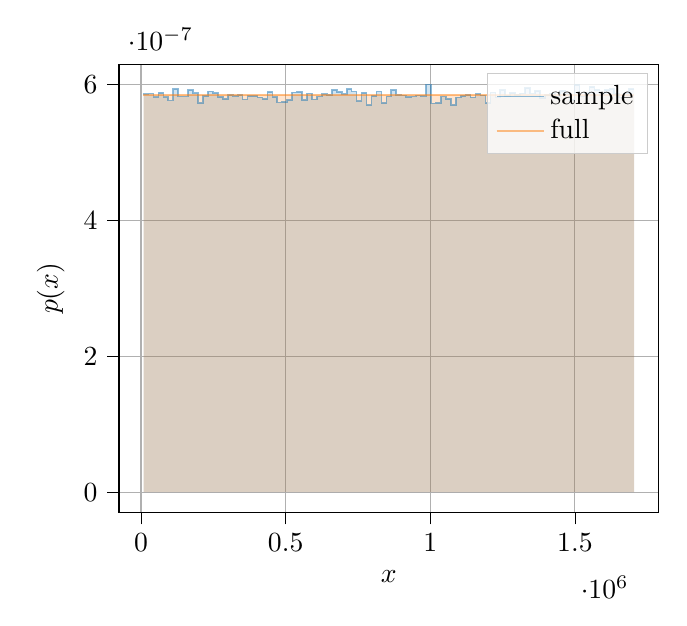
\begin{tikzpicture}

\definecolor{color0}{rgb}{0.12156862745098,0.466666666666667,0.705882352941177}
\definecolor{color1}{rgb}{1,0.498039215686275,0.0549019607843137}

\begin{axis}[
legend cell align={left},
legend style={
  fill opacity=0.8,
  draw opacity=1,
  text opacity=1,
  anchor=north east,
  draw=white!80!black
},
trim axis left,trim axis right,
tick align=outside,
tick pos=left,
x grid style={white!69.0196078431373!black},
xmajorgrids,
xmin=-76238.845, xmax=1789470.825,
xtick style={color=black},
xlabel={\(\displaystyle x\)},
ylabel={\(\displaystyle p(x)\)},
y grid style={white!69.0196078431373!black},
ymajorgrids,
ymin=-2.99677322249481e-08, ymax=6.2932237672391e-07,
ytick style={color=black},
ylabel near ticks
]
\path [fill=color0, fill opacity=0.2]
(axis cs:8566.14,0)
--(axis cs:8566.14,5.83546290983297e-07)
--(axis cs:8566.14,5.85113498443901e-07)
--(axis cs:25698.42,5.85113498443901e-07)
--(axis cs:25698.42,5.85999311356417e-07)
--(axis cs:42830.7,5.85999311356417e-07)
--(axis cs:42830.7,5.80616294426515e-07)
--(axis cs:59962.98,5.80616294426515e-07)
--(axis cs:59962.98,5.87362100452595e-07)
--(axis cs:77095.26,5.87362100452595e-07)
--(axis cs:77095.26,5.80616294426515e-07)
--(axis cs:94227.54,5.80616294426515e-07)
--(axis cs:94227.54,5.75846532589893e-07)
--(axis cs:111359.82,5.75846532589893e-07)
--(axis cs:111359.82,5.9315395411135e-07)
--(axis cs:128492.1,5.9315395411135e-07)
--(axis cs:128492.1,5.81706525703457e-07)
--(axis cs:145624.38,5.81706525703457e-07)
--(axis cs:145624.38,5.81638386248648e-07)
--(axis cs:162756.66,5.81638386248648e-07)
--(axis cs:162756.66,5.91109770467083e-07)
--(axis cs:179888.94,5.91109770467083e-07)
--(axis cs:179888.94,5.86544426994888e-07)
--(axis cs:197021.22,5.86544426994888e-07)
--(axis cs:197021.22,5.7237142039464e-07)
--(axis cs:214153.5,5.7237142039464e-07)
--(axis cs:214153.5,5.82592338615973e-07)
--(axis cs:231285.78,5.82592338615973e-07)
--(axis cs:231285.78,5.89201865732435e-07)
--(axis cs:248418.06,5.89201865732435e-07)
--(axis cs:248418.06,5.87225821542977e-07)
--(axis cs:265550.34,5.87225821542977e-07)
--(axis cs:265550.34,5.81093270610176e-07)
--(axis cs:282682.62,5.81093270610176e-07)
--(axis cs:282682.62,5.78231413508205e-07)
--(axis cs:299814.9,5.78231413508205e-07)
--(axis cs:299814.9,5.84363964441005e-07)
--(axis cs:316947.18,5.84363964441005e-07)
--(axis cs:316947.18,5.82183501887118e-07)
--(axis cs:334079.46,5.82183501887118e-07)
--(axis cs:334079.46,5.83886988257341e-07)
--(axis cs:351211.74,5.83886988257341e-07)
--(axis cs:351211.74,5.77345600595689e-07)
--(axis cs:368344.02,5.77345600595689e-07)
--(axis cs:368344.02,5.82251641341929e-07)
--(axis cs:385476.3,5.82251641341929e-07)
--(axis cs:385476.3,5.82524199161163e-07)
--(axis cs:402608.58,5.82524199161163e-07)
--(axis cs:402608.58,5.80548154971705e-07)
--(axis cs:419740.86,5.80548154971705e-07)
--(axis cs:419740.86,5.78299552963014e-07)
--(axis cs:436873.14,5.78299552963014e-07)
--(axis cs:436873.14,5.88247913365111e-07)
--(axis cs:454005.42,5.88247913365111e-07)
--(axis cs:454005.42,5.81093270610176e-07)
--(axis cs:471137.7,5.81093270610176e-07)
--(axis cs:471137.7,5.7291653603311e-07)
--(axis cs:488269.98,5.7291653603311e-07)
--(axis cs:488269.98,5.73393512216774e-07)
--(axis cs:505402.26,5.73393512216774e-07)
--(axis cs:505402.26,5.76800484957218e-07)
--(axis cs:522534.54,5.76800484957218e-07)
--(axis cs:522534.54,5.87839076636256e-07)
--(axis cs:539666.82,5.87839076636256e-07)
--(axis cs:539666.82,5.88724889548771e-07)
--(axis cs:556799.1,5.88724889548771e-07)
--(axis cs:556799.1,5.76459787683172e-07)
--(axis cs:573931.38,5.76459787683172e-07)
--(axis cs:573931.38,5.86067450811229e-07)
--(axis cs:591063.66,5.86067450811229e-07)
--(axis cs:591063.66,5.77618158414923e-07)
--(axis cs:608195.94,5.77618158414923e-07)
--(axis cs:608195.94,5.81706525703456e-07)
--(axis cs:625328.22,5.81706525703456e-07)
--(axis cs:625328.22,5.85249777353522e-07)
--(axis cs:642460.5,5.85249777353522e-07)
--(axis cs:642460.5,5.83886988257341e-07)
--(axis cs:659592.78,5.83886988257341e-07)
--(axis cs:659592.78,5.91518607195936e-07)
--(axis cs:676725.06,5.91518607195936e-07)
--(axis cs:676725.06,5.88452331729536e-07)
--(axis cs:693857.34,5.88452331729536e-07)
--(axis cs:693857.34,5.85590474627563e-07)
--(axis cs:710989.62,5.85590474627563e-07)
--(axis cs:710989.62,5.92608838472882e-07)
--(axis cs:728121.9,5.92608838472882e-07)
--(axis cs:728121.9,5.89133726277625e-07)
--(axis cs:745254.18,5.89133726277625e-07)
--(axis cs:745254.18,5.74824440767759e-07)
--(axis cs:762386.46,5.74824440767759e-07)
--(axis cs:762386.46,5.87362100452598e-07)
--(axis cs:779518.74,5.87362100452598e-07)
--(axis cs:779518.74,5.69305144928239e-07)
--(axis cs:796651.02,5.69305144928239e-07)
--(axis cs:796651.02,5.82864896435207e-07)
--(axis cs:813783.3,5.82864896435207e-07)
--(axis cs:813783.3,5.88997447368007e-07)
--(axis cs:830915.58,5.88997447368007e-07)
--(axis cs:830915.58,5.72507699304257e-07)
--(axis cs:848047.86,5.72507699304257e-07)
--(axis cs:848047.86,5.81910944067887e-07)
--(axis cs:865180.14,5.81910944067887e-07)
--(axis cs:865180.14,5.91314188831509e-07)
--(axis cs:882312.42,5.91314188831509e-07)
--(axis cs:882312.42,5.83818848802532e-07)
--(axis cs:899444.7,5.83818848802532e-07)
--(axis cs:899444.7,5.83478151528491e-07)
--(axis cs:916576.98,5.83478151528491e-07)
--(axis cs:916576.98,5.80752573336132e-07)
--(axis cs:933709.26,5.80752573336132e-07)
--(axis cs:933709.26,5.81570246793838e-07)
--(axis cs:950841.54,5.81570246793838e-07)
--(axis cs:950841.54,5.83069314799634e-07)
--(axis cs:967973.82,5.83069314799634e-07)
--(axis cs:967973.82,5.8211536243231e-07)
--(axis cs:985106.1,5.8211536243231e-07)
--(axis cs:985106.1,5.99354644498962e-07)
--(axis cs:1002238.38,5.99354644498962e-07)
--(axis cs:1002238.38,5.71758165301359e-07)
--(axis cs:1019370.66,5.71758165301359e-07)
--(axis cs:1019370.66,5.7230328093983e-07)
--(axis cs:1036502.94,5.7230328093983e-07)
--(axis cs:1036502.94,5.81570246793842e-07)
--(axis cs:1053635.22,5.81570246793842e-07)
--(axis cs:1053635.22,5.78231413508203e-07)
--(axis cs:1070767.5,5.78231413508203e-07)
--(axis cs:1070767.5,5.69441423837857e-07)
--(axis cs:1087899.78,5.69441423837857e-07)
--(axis cs:1087899.78,5.80548154971705e-07)
--(axis cs:1105032.06,5.80548154971705e-07)
--(axis cs:1105032.06,5.82387920251545e-07)
--(axis cs:1122164.34,5.82387920251545e-07)
--(axis cs:1122164.34,5.83955127712149e-07)
--(axis cs:1139296.62,5.83955127712149e-07)
--(axis cs:1139296.62,5.80411876062087e-07)
--(axis cs:1156428.9,5.80411876062087e-07)
--(axis cs:1156428.9,5.85454195717953e-07)
--(axis cs:1173561.18,5.85454195717953e-07)
--(axis cs:1173561.18,5.83478151528487e-07)
--(axis cs:1190693.46,5.83478151528487e-07)
--(axis cs:1190693.46,5.72439559849448e-07)
--(axis cs:1207825.74,5.72439559849448e-07)
--(axis cs:1207825.74,5.8756651881702e-07)
--(axis cs:1224958.02,5.8756651881702e-07)
--(axis cs:1224958.02,5.8027559715247e-07)
--(axis cs:1242090.3,5.8027559715247e-07)
--(axis cs:1242090.3,5.90973491557465e-07)
--(axis cs:1259222.58,5.90973491557465e-07)
--(axis cs:1259222.58,5.83001175344825e-07)
--(axis cs:1276354.86,5.83001175344825e-07)
--(axis cs:1276354.86,5.87225821542984e-07)
--(axis cs:1293487.14,5.87225821542984e-07)
--(axis cs:1293487.14,5.84227685531385e-07)
--(axis cs:1310619.42,5.84227685531385e-07)
--(axis cs:1310619.42,5.86271869175651e-07)
--(axis cs:1327751.7,5.86271869175651e-07)
--(axis cs:1327751.7,5.94653022117144e-07)
--(axis cs:1344883.98,5.94653022117144e-07)
--(axis cs:1344883.98,5.86203729720843e-07)
--(axis cs:1362016.26,5.86203729720843e-07)
--(axis cs:1362016.26,5.89815120825714e-07)
--(axis cs:1379148.54,5.89815120825714e-07)
--(axis cs:1379148.54,5.7966234205919e-07)
--(axis cs:1396280.82,5.7966234205919e-07)
--(axis cs:1396280.82,5.83750709347723e-07)
--(axis cs:1413413.1,5.83750709347723e-07)
--(axis cs:1413413.1,5.85999311356416e-07)
--(axis cs:1430545.38,5.85999311356416e-07)
--(axis cs:1430545.38,5.82047222977509e-07)
--(axis cs:1447677.66,5.82047222977509e-07)
--(axis cs:1447677.66,5.89542563006478e-07)
--(axis cs:1464809.94,5.89542563006478e-07)
--(axis cs:1464809.94,5.85045358989092e-07)
--(axis cs:1481942.22,5.85045358989092e-07)
--(axis cs:1481942.22,5.76800484957216e-07)
--(axis cs:1499074.5,5.76800484957216e-07)
--(axis cs:1499074.5,5.9860511049606e-07)
--(axis cs:1516206.78,5.9860511049606e-07)
--(axis cs:1516206.78,5.81910944067883e-07)
--(axis cs:1533339.06,5.81910944067883e-07)
--(axis cs:1533339.06,5.87157682088167e-07)
--(axis cs:1550471.34,5.87157682088167e-07)
--(axis cs:1550471.34,5.96083950668139e-07)
--(axis cs:1567603.62,5.96083950668139e-07)
--(axis cs:1567603.62,5.91791165015171e-07)
--(axis cs:1584735.9,5.91791165015171e-07)
--(axis cs:1584735.9,5.83546290983296e-07)
--(axis cs:1601868.18,5.83546290983296e-07)
--(axis cs:1601868.18,5.91723025560362e-07)
--(axis cs:1619000.46,5.91723025560362e-07)
--(axis cs:1619000.46,5.9247255956326e-07)
--(axis cs:1636132.74,5.9247255956326e-07)
--(axis cs:1636132.74,5.85249777353518e-07)
--(axis cs:1653265.02,5.85249777353518e-07)
--(axis cs:1653265.02,5.8027559715247e-07)
--(axis cs:1670397.3,5.8027559715247e-07)
--(axis cs:1670397.3,5.86408148085269e-07)
--(axis cs:1687529.58,5.86408148085269e-07)
--(axis cs:1687529.58,5.93153954111349e-07)
--(axis cs:1704661.86,5.93153954111349e-07)
--(axis cs:1704661.86,0)
--(axis cs:1704661.86,0)
--(axis cs:1687529.58,0)
--(axis cs:1687529.58,0)
--(axis cs:1670397.3,0)
--(axis cs:1670397.3,0)
--(axis cs:1653265.02,0)
--(axis cs:1653265.02,0)
--(axis cs:1636132.74,0)
--(axis cs:1636132.74,0)
--(axis cs:1619000.46,0)
--(axis cs:1619000.46,0)
--(axis cs:1601868.18,0)
--(axis cs:1601868.18,0)
--(axis cs:1584735.9,0)
--(axis cs:1584735.9,0)
--(axis cs:1567603.62,0)
--(axis cs:1567603.62,0)
--(axis cs:1550471.34,0)
--(axis cs:1550471.34,0)
--(axis cs:1533339.06,0)
--(axis cs:1533339.06,0)
--(axis cs:1516206.78,0)
--(axis cs:1516206.78,0)
--(axis cs:1499074.5,0)
--(axis cs:1499074.5,0)
--(axis cs:1481942.22,0)
--(axis cs:1481942.22,0)
--(axis cs:1464809.94,0)
--(axis cs:1464809.94,0)
--(axis cs:1447677.66,0)
--(axis cs:1447677.66,0)
--(axis cs:1430545.38,0)
--(axis cs:1430545.38,0)
--(axis cs:1413413.1,0)
--(axis cs:1413413.1,0)
--(axis cs:1396280.82,0)
--(axis cs:1396280.82,0)
--(axis cs:1379148.54,0)
--(axis cs:1379148.54,0)
--(axis cs:1362016.26,0)
--(axis cs:1362016.26,0)
--(axis cs:1344883.98,0)
--(axis cs:1344883.98,0)
--(axis cs:1327751.7,0)
--(axis cs:1327751.7,0)
--(axis cs:1310619.42,0)
--(axis cs:1310619.42,0)
--(axis cs:1293487.14,0)
--(axis cs:1293487.14,0)
--(axis cs:1276354.86,0)
--(axis cs:1276354.86,0)
--(axis cs:1259222.58,0)
--(axis cs:1259222.58,0)
--(axis cs:1242090.3,0)
--(axis cs:1242090.3,0)
--(axis cs:1224958.02,0)
--(axis cs:1224958.02,0)
--(axis cs:1207825.74,0)
--(axis cs:1207825.74,0)
--(axis cs:1190693.46,0)
--(axis cs:1190693.46,0)
--(axis cs:1173561.18,0)
--(axis cs:1173561.18,0)
--(axis cs:1156428.9,0)
--(axis cs:1156428.9,0)
--(axis cs:1139296.62,0)
--(axis cs:1139296.62,0)
--(axis cs:1122164.34,0)
--(axis cs:1122164.34,0)
--(axis cs:1105032.06,0)
--(axis cs:1105032.06,0)
--(axis cs:1087899.78,0)
--(axis cs:1087899.78,0)
--(axis cs:1070767.5,0)
--(axis cs:1070767.5,0)
--(axis cs:1053635.22,0)
--(axis cs:1053635.22,0)
--(axis cs:1036502.94,0)
--(axis cs:1036502.94,0)
--(axis cs:1019370.66,0)
--(axis cs:1019370.66,0)
--(axis cs:1002238.38,0)
--(axis cs:1002238.38,0)
--(axis cs:985106.1,0)
--(axis cs:985106.1,0)
--(axis cs:967973.82,0)
--(axis cs:967973.82,0)
--(axis cs:950841.54,0)
--(axis cs:950841.54,0)
--(axis cs:933709.26,0)
--(axis cs:933709.26,0)
--(axis cs:916576.98,0)
--(axis cs:916576.98,0)
--(axis cs:899444.7,0)
--(axis cs:899444.7,0)
--(axis cs:882312.42,0)
--(axis cs:882312.42,0)
--(axis cs:865180.14,0)
--(axis cs:865180.14,0)
--(axis cs:848047.86,0)
--(axis cs:848047.86,0)
--(axis cs:830915.58,0)
--(axis cs:830915.58,0)
--(axis cs:813783.3,0)
--(axis cs:813783.3,0)
--(axis cs:796651.02,0)
--(axis cs:796651.02,0)
--(axis cs:779518.74,0)
--(axis cs:779518.74,0)
--(axis cs:762386.46,0)
--(axis cs:762386.46,0)
--(axis cs:745254.18,0)
--(axis cs:745254.18,0)
--(axis cs:728121.9,0)
--(axis cs:728121.9,0)
--(axis cs:710989.62,0)
--(axis cs:710989.62,0)
--(axis cs:693857.34,0)
--(axis cs:693857.34,0)
--(axis cs:676725.06,0)
--(axis cs:676725.06,0)
--(axis cs:659592.78,0)
--(axis cs:659592.78,0)
--(axis cs:642460.5,0)
--(axis cs:642460.5,0)
--(axis cs:625328.22,0)
--(axis cs:625328.22,0)
--(axis cs:608195.94,0)
--(axis cs:608195.94,0)
--(axis cs:591063.66,0)
--(axis cs:591063.66,0)
--(axis cs:573931.38,0)
--(axis cs:573931.38,0)
--(axis cs:556799.1,0)
--(axis cs:556799.1,0)
--(axis cs:539666.82,0)
--(axis cs:539666.82,0)
--(axis cs:522534.54,0)
--(axis cs:522534.54,0)
--(axis cs:505402.26,0)
--(axis cs:505402.26,0)
--(axis cs:488269.98,0)
--(axis cs:488269.98,0)
--(axis cs:471137.7,0)
--(axis cs:471137.7,0)
--(axis cs:454005.42,0)
--(axis cs:454005.42,0)
--(axis cs:436873.14,0)
--(axis cs:436873.14,0)
--(axis cs:419740.86,0)
--(axis cs:419740.86,0)
--(axis cs:402608.58,0)
--(axis cs:402608.58,0)
--(axis cs:385476.3,0)
--(axis cs:385476.3,0)
--(axis cs:368344.02,0)
--(axis cs:368344.02,0)
--(axis cs:351211.74,0)
--(axis cs:351211.74,0)
--(axis cs:334079.46,0)
--(axis cs:334079.46,0)
--(axis cs:316947.18,0)
--(axis cs:316947.18,0)
--(axis cs:299814.9,0)
--(axis cs:299814.9,0)
--(axis cs:282682.62,0)
--(axis cs:282682.62,0)
--(axis cs:265550.34,0)
--(axis cs:265550.34,0)
--(axis cs:248418.06,0)
--(axis cs:248418.06,0)
--(axis cs:231285.78,0)
--(axis cs:231285.78,0)
--(axis cs:214153.5,0)
--(axis cs:214153.5,0)
--(axis cs:197021.22,0)
--(axis cs:197021.22,0)
--(axis cs:179888.94,0)
--(axis cs:179888.94,0)
--(axis cs:162756.66,0)
--(axis cs:162756.66,0)
--(axis cs:145624.38,0)
--(axis cs:145624.38,0)
--(axis cs:128492.1,0)
--(axis cs:128492.1,0)
--(axis cs:111359.82,0)
--(axis cs:111359.82,0)
--(axis cs:94227.54,0)
--(axis cs:94227.54,0)
--(axis cs:77095.26,0)
--(axis cs:77095.26,0)
--(axis cs:59962.98,0)
--(axis cs:59962.98,0)
--(axis cs:42830.7,0)
--(axis cs:42830.7,0)
--(axis cs:25698.42,0)
--(axis cs:25698.42,0)
--(axis cs:8566.14,0)
--(axis cs:8566.14,0)
--cycle;

\path [fill=color1, fill opacity=0.2]
(axis cs:8566.16,0)
--(axis cs:8566.16,5.8371493606733e-07)
--(axis cs:8566.16,5.83680866439357e-07)
--(axis cs:25698.48,5.83680866439357e-07)
--(axis cs:25698.48,5.83680866439357e-07)
--(axis cs:42830.8,5.83680866439357e-07)
--(axis cs:42830.8,5.8371493606733e-07)
--(axis cs:59963.12,5.8371493606733e-07)
--(axis cs:59963.12,5.83680866439357e-07)
--(axis cs:77095.44,5.83680866439357e-07)
--(axis cs:77095.44,5.83680866439357e-07)
--(axis cs:94227.76,5.83680866439357e-07)
--(axis cs:94227.76,5.83714936067331e-07)
--(axis cs:111360.08,5.83714936067331e-07)
--(axis cs:111360.08,5.83680866439357e-07)
--(axis cs:128492.4,5.83680866439357e-07)
--(axis cs:128492.4,5.83680866439357e-07)
--(axis cs:145624.72,5.83680866439357e-07)
--(axis cs:145624.72,5.8371493606733e-07)
--(axis cs:162757.04,5.8371493606733e-07)
--(axis cs:162757.04,5.83680866439358e-07)
--(axis cs:179889.36,5.83680866439358e-07)
--(axis cs:179889.36,5.83680866439357e-07)
--(axis cs:197021.68,5.83680866439357e-07)
--(axis cs:197021.68,5.8371493606733e-07)
--(axis cs:214154,5.8371493606733e-07)
--(axis cs:214154,5.83680866439358e-07)
--(axis cs:231286.32,5.83680866439358e-07)
--(axis cs:231286.32,5.83680866439357e-07)
--(axis cs:248418.64,5.83680866439357e-07)
--(axis cs:248418.64,5.8371493606733e-07)
--(axis cs:265550.96,5.8371493606733e-07)
--(axis cs:265550.96,5.83680866439357e-07)
--(axis cs:282683.28,5.83680866439357e-07)
--(axis cs:282683.28,5.83680866439357e-07)
--(axis cs:299815.6,5.83680866439357e-07)
--(axis cs:299815.6,5.8371493606733e-07)
--(axis cs:316947.92,5.8371493606733e-07)
--(axis cs:316947.92,5.83680866439357e-07)
--(axis cs:334080.24,5.83680866439357e-07)
--(axis cs:334080.24,5.83680866439359e-07)
--(axis cs:351212.56,5.83680866439359e-07)
--(axis cs:351212.56,5.8371493606733e-07)
--(axis cs:368344.88,5.8371493606733e-07)
--(axis cs:368344.88,5.83680866439357e-07)
--(axis cs:385477.2,5.83680866439357e-07)
--(axis cs:385477.2,5.83680866439357e-07)
--(axis cs:402609.52,5.83680866439357e-07)
--(axis cs:402609.52,5.83680866439357e-07)
--(axis cs:419741.84,5.83680866439357e-07)
--(axis cs:419741.84,5.8371493606733e-07)
--(axis cs:436874.16,5.8371493606733e-07)
--(axis cs:436874.16,5.83680866439357e-07)
--(axis cs:454006.48,5.83680866439357e-07)
--(axis cs:454006.48,5.83680866439359e-07)
--(axis cs:471138.8,5.83680866439359e-07)
--(axis cs:471138.8,5.8371493606733e-07)
--(axis cs:488271.12,5.8371493606733e-07)
--(axis cs:488271.12,5.83680866439357e-07)
--(axis cs:505403.44,5.83680866439357e-07)
--(axis cs:505403.44,5.83680866439355e-07)
--(axis cs:522535.76,5.83680866439355e-07)
--(axis cs:522535.76,5.83714936067332e-07)
--(axis cs:539668.08,5.83714936067332e-07)
--(axis cs:539668.08,5.83680866439359e-07)
--(axis cs:556800.4,5.83680866439359e-07)
--(axis cs:556800.4,5.83680866439355e-07)
--(axis cs:573932.72,5.83680866439355e-07)
--(axis cs:573932.72,5.83714936067332e-07)
--(axis cs:591065.04,5.83714936067332e-07)
--(axis cs:591065.04,5.83680866439355e-07)
--(axis cs:608197.36,5.83680866439355e-07)
--(axis cs:608197.36,5.83680866439359e-07)
--(axis cs:625329.68,5.83680866439359e-07)
--(axis cs:625329.68,5.83714936067328e-07)
--(axis cs:642462,5.83714936067328e-07)
--(axis cs:642462,5.83680866439359e-07)
--(axis cs:659594.32,5.83680866439359e-07)
--(axis cs:659594.32,5.83680866439355e-07)
--(axis cs:676726.64,5.83680866439355e-07)
--(axis cs:676726.64,5.83714936067332e-07)
--(axis cs:693858.96,5.83714936067332e-07)
--(axis cs:693858.96,5.83680866439359e-07)
--(axis cs:710991.28,5.83680866439359e-07)
--(axis cs:710991.28,5.83680866439355e-07)
--(axis cs:728123.6,5.83680866439355e-07)
--(axis cs:728123.6,5.83714936067332e-07)
--(axis cs:745255.92,5.83714936067332e-07)
--(axis cs:745255.92,5.83680866439355e-07)
--(axis cs:762388.24,5.83680866439355e-07)
--(axis cs:762388.24,5.83680866439359e-07)
--(axis cs:779520.56,5.83680866439359e-07)
--(axis cs:779520.56,5.83714936067328e-07)
--(axis cs:796652.88,5.83714936067328e-07)
--(axis cs:796652.88,5.83680866439359e-07)
--(axis cs:813785.2,5.83680866439359e-07)
--(axis cs:813785.2,5.83680866439359e-07)
--(axis cs:830917.52,5.83680866439359e-07)
--(axis cs:830917.52,5.83680866439355e-07)
--(axis cs:848049.84,5.83680866439355e-07)
--(axis cs:848049.84,5.83714936067332e-07)
--(axis cs:865182.16,5.83714936067332e-07)
--(axis cs:865182.16,5.83680866439355e-07)
--(axis cs:882314.48,5.83680866439355e-07)
--(axis cs:882314.48,5.83680866439359e-07)
--(axis cs:899446.8,5.83680866439359e-07)
--(axis cs:899446.8,5.83714936067328e-07)
--(axis cs:916579.12,5.83714936067328e-07)
--(axis cs:916579.12,5.83680866439359e-07)
--(axis cs:933711.44,5.83680866439359e-07)
--(axis cs:933711.44,5.83680866439359e-07)
--(axis cs:950843.76,5.83680866439359e-07)
--(axis cs:950843.76,5.83714936067328e-07)
--(axis cs:967976.08,5.83714936067328e-07)
--(axis cs:967976.08,5.83680866439359e-07)
--(axis cs:985108.4,5.83680866439359e-07)
--(axis cs:985108.4,5.83680866439355e-07)
--(axis cs:1002240.72,5.83680866439355e-07)
--(axis cs:1002240.72,5.83714936067332e-07)
--(axis cs:1019373.04,5.83714936067332e-07)
--(axis cs:1019373.04,5.83680866439355e-07)
--(axis cs:1036505.36,5.83680866439355e-07)
--(axis cs:1036505.36,5.83680866439355e-07)
--(axis cs:1053637.68,5.83680866439355e-07)
--(axis cs:1053637.68,5.83714936067336e-07)
--(axis cs:1070770,5.83714936067336e-07)
--(axis cs:1070770,5.83680866439355e-07)
--(axis cs:1087902.32,5.83680866439355e-07)
--(axis cs:1087902.32,5.83680866439355e-07)
--(axis cs:1105034.64,5.83680866439355e-07)
--(axis cs:1105034.64,5.83714936067336e-07)
--(axis cs:1122166.96,5.83714936067336e-07)
--(axis cs:1122166.96,5.83680866439355e-07)
--(axis cs:1139299.28,5.83680866439355e-07)
--(axis cs:1139299.28,5.83680866439355e-07)
--(axis cs:1156431.6,5.83680866439355e-07)
--(axis cs:1156431.6,5.83714936067328e-07)
--(axis cs:1173563.92,5.83714936067328e-07)
--(axis cs:1173563.92,5.83680866439363e-07)
--(axis cs:1190696.24,5.83680866439363e-07)
--(axis cs:1190696.24,5.83680866439355e-07)
--(axis cs:1207828.56,5.83680866439355e-07)
--(axis cs:1207828.56,5.83714936067328e-07)
--(axis cs:1224960.88,5.83714936067328e-07)
--(axis cs:1224960.88,5.83680866439363e-07)
--(axis cs:1242093.2,5.83680866439363e-07)
--(axis cs:1242093.2,5.83680866439355e-07)
--(axis cs:1259225.52,5.83680866439355e-07)
--(axis cs:1259225.52,5.83680866439355e-07)
--(axis cs:1276357.84,5.83680866439355e-07)
--(axis cs:1276357.84,5.83714936067328e-07)
--(axis cs:1293490.16,5.83714936067328e-07)
--(axis cs:1293490.16,5.83680866439363e-07)
--(axis cs:1310622.48,5.83680866439363e-07)
--(axis cs:1310622.48,5.83680866439355e-07)
--(axis cs:1327754.8,5.83680866439355e-07)
--(axis cs:1327754.8,5.83714936067328e-07)
--(axis cs:1344887.12,5.83714936067328e-07)
--(axis cs:1344887.12,5.83680866439355e-07)
--(axis cs:1362019.44,5.83680866439355e-07)
--(axis cs:1362019.44,5.83680866439363e-07)
--(axis cs:1379151.76,5.83680866439363e-07)
--(axis cs:1379151.76,5.83714936067328e-07)
--(axis cs:1396284.08,5.83714936067328e-07)
--(axis cs:1396284.08,5.83680866439355e-07)
--(axis cs:1413416.4,5.83680866439355e-07)
--(axis cs:1413416.4,5.83680866439363e-07)
--(axis cs:1430548.72,5.83680866439363e-07)
--(axis cs:1430548.72,5.83714936067328e-07)
--(axis cs:1447681.04,5.83714936067328e-07)
--(axis cs:1447681.04,5.83680866439355e-07)
--(axis cs:1464813.36,5.83680866439355e-07)
--(axis cs:1464813.36,5.83680866439355e-07)
--(axis cs:1481945.68,5.83680866439355e-07)
--(axis cs:1481945.68,5.83714936067336e-07)
--(axis cs:1499078,5.83714936067336e-07)
--(axis cs:1499078,5.83680866439355e-07)
--(axis cs:1516210.32,5.83680866439355e-07)
--(axis cs:1516210.32,5.83680866439355e-07)
--(axis cs:1533342.64,5.83680866439355e-07)
--(axis cs:1533342.64,5.83714936067336e-07)
--(axis cs:1550474.96,5.83714936067336e-07)
--(axis cs:1550474.96,5.83680866439355e-07)
--(axis cs:1567607.28,5.83680866439355e-07)
--(axis cs:1567607.28,5.83680866439355e-07)
--(axis cs:1584739.6,5.83680866439355e-07)
--(axis cs:1584739.6,5.83714936067328e-07)
--(axis cs:1601871.92,5.83714936067328e-07)
--(axis cs:1601871.92,5.83680866439363e-07)
--(axis cs:1619004.24,5.83680866439363e-07)
--(axis cs:1619004.24,5.83680866439355e-07)
--(axis cs:1636136.56,5.83680866439355e-07)
--(axis cs:1636136.56,5.83714936067328e-07)
--(axis cs:1653268.88,5.83714936067328e-07)
--(axis cs:1653268.88,5.83680866439363e-07)
--(axis cs:1670401.2,5.83680866439363e-07)
--(axis cs:1670401.2,5.83680866439355e-07)
--(axis cs:1687533.52,5.83680866439355e-07)
--(axis cs:1687533.52,5.83714936067328e-07)
--(axis cs:1704665.84,5.83714936067328e-07)
--(axis cs:1704665.84,0)
--(axis cs:1704665.84,0)
--(axis cs:1687533.52,0)
--(axis cs:1687533.52,0)
--(axis cs:1670401.2,0)
--(axis cs:1670401.2,0)
--(axis cs:1653268.88,0)
--(axis cs:1653268.88,0)
--(axis cs:1636136.56,0)
--(axis cs:1636136.56,0)
--(axis cs:1619004.24,0)
--(axis cs:1619004.24,0)
--(axis cs:1601871.92,0)
--(axis cs:1601871.92,0)
--(axis cs:1584739.6,0)
--(axis cs:1584739.6,0)
--(axis cs:1567607.28,0)
--(axis cs:1567607.28,0)
--(axis cs:1550474.96,0)
--(axis cs:1550474.96,0)
--(axis cs:1533342.64,0)
--(axis cs:1533342.64,0)
--(axis cs:1516210.32,0)
--(axis cs:1516210.32,0)
--(axis cs:1499078,0)
--(axis cs:1499078,0)
--(axis cs:1481945.68,0)
--(axis cs:1481945.68,0)
--(axis cs:1464813.36,0)
--(axis cs:1464813.36,0)
--(axis cs:1447681.04,0)
--(axis cs:1447681.04,0)
--(axis cs:1430548.72,0)
--(axis cs:1430548.72,0)
--(axis cs:1413416.4,0)
--(axis cs:1413416.4,0)
--(axis cs:1396284.08,0)
--(axis cs:1396284.08,0)
--(axis cs:1379151.76,0)
--(axis cs:1379151.76,0)
--(axis cs:1362019.44,0)
--(axis cs:1362019.44,0)
--(axis cs:1344887.12,0)
--(axis cs:1344887.12,0)
--(axis cs:1327754.8,0)
--(axis cs:1327754.8,0)
--(axis cs:1310622.48,0)
--(axis cs:1310622.48,0)
--(axis cs:1293490.16,0)
--(axis cs:1293490.16,0)
--(axis cs:1276357.84,0)
--(axis cs:1276357.84,0)
--(axis cs:1259225.52,0)
--(axis cs:1259225.52,0)
--(axis cs:1242093.2,0)
--(axis cs:1242093.2,0)
--(axis cs:1224960.88,0)
--(axis cs:1224960.88,0)
--(axis cs:1207828.56,0)
--(axis cs:1207828.56,0)
--(axis cs:1190696.24,0)
--(axis cs:1190696.24,0)
--(axis cs:1173563.92,0)
--(axis cs:1173563.92,0)
--(axis cs:1156431.6,0)
--(axis cs:1156431.6,0)
--(axis cs:1139299.28,0)
--(axis cs:1139299.28,0)
--(axis cs:1122166.96,0)
--(axis cs:1122166.96,0)
--(axis cs:1105034.64,0)
--(axis cs:1105034.64,0)
--(axis cs:1087902.32,0)
--(axis cs:1087902.32,0)
--(axis cs:1070770,0)
--(axis cs:1070770,0)
--(axis cs:1053637.68,0)
--(axis cs:1053637.68,0)
--(axis cs:1036505.36,0)
--(axis cs:1036505.36,0)
--(axis cs:1019373.04,0)
--(axis cs:1019373.04,0)
--(axis cs:1002240.72,0)
--(axis cs:1002240.72,0)
--(axis cs:985108.4,0)
--(axis cs:985108.4,0)
--(axis cs:967976.08,0)
--(axis cs:967976.08,0)
--(axis cs:950843.76,0)
--(axis cs:950843.76,0)
--(axis cs:933711.44,0)
--(axis cs:933711.44,0)
--(axis cs:916579.12,0)
--(axis cs:916579.12,0)
--(axis cs:899446.8,0)
--(axis cs:899446.8,0)
--(axis cs:882314.48,0)
--(axis cs:882314.48,0)
--(axis cs:865182.16,0)
--(axis cs:865182.16,0)
--(axis cs:848049.84,0)
--(axis cs:848049.84,0)
--(axis cs:830917.52,0)
--(axis cs:830917.52,0)
--(axis cs:813785.2,0)
--(axis cs:813785.2,0)
--(axis cs:796652.88,0)
--(axis cs:796652.88,0)
--(axis cs:779520.56,0)
--(axis cs:779520.56,0)
--(axis cs:762388.24,0)
--(axis cs:762388.24,0)
--(axis cs:745255.92,0)
--(axis cs:745255.92,0)
--(axis cs:728123.6,0)
--(axis cs:728123.6,0)
--(axis cs:710991.28,0)
--(axis cs:710991.28,0)
--(axis cs:693858.96,0)
--(axis cs:693858.96,0)
--(axis cs:676726.64,0)
--(axis cs:676726.64,0)
--(axis cs:659594.32,0)
--(axis cs:659594.32,0)
--(axis cs:642462,0)
--(axis cs:642462,0)
--(axis cs:625329.68,0)
--(axis cs:625329.68,0)
--(axis cs:608197.36,0)
--(axis cs:608197.36,0)
--(axis cs:591065.04,0)
--(axis cs:591065.04,0)
--(axis cs:573932.72,0)
--(axis cs:573932.72,0)
--(axis cs:556800.4,0)
--(axis cs:556800.4,0)
--(axis cs:539668.08,0)
--(axis cs:539668.08,0)
--(axis cs:522535.76,0)
--(axis cs:522535.76,0)
--(axis cs:505403.44,0)
--(axis cs:505403.44,0)
--(axis cs:488271.12,0)
--(axis cs:488271.12,0)
--(axis cs:471138.8,0)
--(axis cs:471138.8,0)
--(axis cs:454006.48,0)
--(axis cs:454006.48,0)
--(axis cs:436874.16,0)
--(axis cs:436874.16,0)
--(axis cs:419741.84,0)
--(axis cs:419741.84,0)
--(axis cs:402609.52,0)
--(axis cs:402609.52,0)
--(axis cs:385477.2,0)
--(axis cs:385477.2,0)
--(axis cs:368344.88,0)
--(axis cs:368344.88,0)
--(axis cs:351212.56,0)
--(axis cs:351212.56,0)
--(axis cs:334080.24,0)
--(axis cs:334080.24,0)
--(axis cs:316947.92,0)
--(axis cs:316947.92,0)
--(axis cs:299815.6,0)
--(axis cs:299815.6,0)
--(axis cs:282683.28,0)
--(axis cs:282683.28,0)
--(axis cs:265550.96,0)
--(axis cs:265550.96,0)
--(axis cs:248418.64,0)
--(axis cs:248418.64,0)
--(axis cs:231286.32,0)
--(axis cs:231286.32,0)
--(axis cs:214154,0)
--(axis cs:214154,0)
--(axis cs:197021.68,0)
--(axis cs:197021.68,0)
--(axis cs:179889.36,0)
--(axis cs:179889.36,0)
--(axis cs:162757.04,0)
--(axis cs:162757.04,0)
--(axis cs:145624.72,0)
--(axis cs:145624.72,0)
--(axis cs:128492.4,0)
--(axis cs:128492.4,0)
--(axis cs:111360.08,0)
--(axis cs:111360.08,0)
--(axis cs:94227.76,0)
--(axis cs:94227.76,0)
--(axis cs:77095.44,0)
--(axis cs:77095.44,0)
--(axis cs:59963.12,0)
--(axis cs:59963.12,0)
--(axis cs:42830.8,0)
--(axis cs:42830.8,0)
--(axis cs:25698.48,0)
--(axis cs:25698.48,0)
--(axis cs:8566.16,0)
--(axis cs:8566.16,0)
--cycle;

\addplot [semithick, color0, const plot mark right, opacity=0.5]
table {%
8566.14 5.83546290983297e-07
25698.42 5.85113498443901e-07
42830.7 5.85999311356417e-07
59962.98 5.80616294426515e-07
77095.26 5.87362100452595e-07
94227.54 5.80616294426515e-07
111359.82 5.75846532589893e-07
128492.1 5.9315395411135e-07
145624.38 5.81706525703457e-07
162756.66 5.81638386248648e-07
179888.94 5.91109770467083e-07
197021.22 5.86544426994888e-07
214153.5 5.7237142039464e-07
231285.78 5.82592338615973e-07
248418.06 5.89201865732435e-07
265550.34 5.87225821542977e-07
282682.62 5.81093270610176e-07
299814.9 5.78231413508205e-07
316947.18 5.84363964441005e-07
334079.46 5.82183501887118e-07
351211.74 5.83886988257341e-07
368344.02 5.77345600595689e-07
385476.3 5.82251641341929e-07
402608.58 5.82524199161163e-07
419740.86 5.80548154971705e-07
436873.14 5.78299552963014e-07
454005.42 5.88247913365111e-07
471137.7 5.81093270610176e-07
488269.98 5.7291653603311e-07
505402.26 5.73393512216774e-07
522534.54 5.76800484957218e-07
539666.82 5.87839076636256e-07
556799.1 5.88724889548771e-07
573931.38 5.76459787683172e-07
591063.66 5.86067450811229e-07
608195.94 5.77618158414923e-07
625328.22 5.81706525703456e-07
642460.5 5.85249777353522e-07
659592.78 5.83886988257341e-07
676725.06 5.91518607195936e-07
693857.34 5.88452331729536e-07
710989.62 5.85590474627563e-07
728121.9 5.92608838472882e-07
745254.18 5.89133726277625e-07
762386.46 5.74824440767759e-07
779518.74 5.87362100452598e-07
796651.02 5.69305144928239e-07
813783.3 5.82864896435207e-07
830915.58 5.88997447368007e-07
848047.86 5.72507699304257e-07
865180.14 5.81910944067887e-07
882312.42 5.91314188831509e-07
899444.7 5.83818848802532e-07
916576.98 5.83478151528491e-07
933709.26 5.80752573336132e-07
950841.54 5.81570246793838e-07
967973.82 5.83069314799634e-07
985106.1 5.8211536243231e-07
1002238.38 5.99354644498962e-07
1019370.66 5.71758165301359e-07
1036502.94 5.7230328093983e-07
1053635.22 5.81570246793842e-07
1070767.5 5.78231413508203e-07
1087899.78 5.69441423837857e-07
1105032.06 5.80548154971705e-07
1122164.34 5.82387920251545e-07
1139296.62 5.83955127712149e-07
1156428.9 5.80411876062087e-07
1173561.18 5.85454195717953e-07
1190693.46 5.83478151528487e-07
1207825.74 5.72439559849448e-07
1224958.02 5.8756651881702e-07
1242090.3 5.8027559715247e-07
1259222.58 5.90973491557465e-07
1276354.86 5.83001175344825e-07
1293487.14 5.87225821542984e-07
1310619.42 5.84227685531385e-07
1327751.7 5.86271869175651e-07
1344883.98 5.94653022117144e-07
1362016.26 5.86203729720843e-07
1379148.54 5.89815120825714e-07
1396280.82 5.7966234205919e-07
1413413.1 5.83750709347723e-07
1430545.38 5.85999311356416e-07
1447677.66 5.82047222977509e-07
1464809.94 5.89542563006478e-07
1481942.22 5.85045358989092e-07
1499074.5 5.76800484957216e-07
1516206.78 5.9860511049606e-07
1533339.06 5.81910944067883e-07
1550471.34 5.87157682088167e-07
1567603.62 5.96083950668139e-07
1584735.9 5.91791165015171e-07
1601868.18 5.83546290983296e-07
1619000.46 5.91723025560362e-07
1636132.74 5.9247255956326e-07
1653265.02 5.85249777353518e-07
1670397.3 5.8027559715247e-07
1687529.58 5.86408148085269e-07
1704661.86 5.93153954111349e-07
};
\addlegendentry{sample}
\addplot [semithick, color1, const plot mark right, opacity=0.5]
table {%
8566.16 5.8371493606733e-07
25698.48 5.83680866439357e-07
42830.8 5.83680866439357e-07
59963.12 5.8371493606733e-07
77095.44 5.83680866439357e-07
94227.76 5.83680866439357e-07
111360.08 5.83714936067331e-07
128492.4 5.83680866439357e-07
145624.72 5.83680866439357e-07
162757.04 5.8371493606733e-07
179889.36 5.83680866439358e-07
197021.68 5.83680866439357e-07
214154 5.8371493606733e-07
231286.32 5.83680866439358e-07
248418.64 5.83680866439357e-07
265550.96 5.8371493606733e-07
282683.28 5.83680866439357e-07
299815.6 5.83680866439357e-07
316947.92 5.8371493606733e-07
334080.24 5.83680866439357e-07
351212.56 5.83680866439359e-07
368344.88 5.8371493606733e-07
385477.2 5.83680866439357e-07
402609.52 5.83680866439357e-07
419741.84 5.83680866439357e-07
436874.16 5.8371493606733e-07
454006.48 5.83680866439357e-07
471138.8 5.83680866439359e-07
488271.12 5.8371493606733e-07
505403.44 5.83680866439357e-07
522535.76 5.83680866439355e-07
539668.08 5.83714936067332e-07
556800.4 5.83680866439359e-07
573932.72 5.83680866439355e-07
591065.04 5.83714936067332e-07
608197.36 5.83680866439355e-07
625329.68 5.83680866439359e-07
642462 5.83714936067328e-07
659594.32 5.83680866439359e-07
676726.64 5.83680866439355e-07
693858.96 5.83714936067332e-07
710991.28 5.83680866439359e-07
728123.6 5.83680866439355e-07
745255.92 5.83714936067332e-07
762388.24 5.83680866439355e-07
779520.56 5.83680866439359e-07
796652.88 5.83714936067328e-07
813785.2 5.83680866439359e-07
830917.52 5.83680866439359e-07
848049.84 5.83680866439355e-07
865182.16 5.83714936067332e-07
882314.48 5.83680866439355e-07
899446.8 5.83680866439359e-07
916579.12 5.83714936067328e-07
933711.44 5.83680866439359e-07
950843.76 5.83680866439359e-07
967976.08 5.83714936067328e-07
985108.4 5.83680866439359e-07
1002240.72 5.83680866439355e-07
1019373.04 5.83714936067332e-07
1036505.36 5.83680866439355e-07
1053637.68 5.83680866439355e-07
1070770 5.83714936067336e-07
1087902.32 5.83680866439355e-07
1105034.64 5.83680866439355e-07
1122166.96 5.83714936067336e-07
1139299.28 5.83680866439355e-07
1156431.6 5.83680866439355e-07
1173563.92 5.83714936067328e-07
1190696.24 5.83680866439363e-07
1207828.56 5.83680866439355e-07
1224960.88 5.83714936067328e-07
1242093.2 5.83680866439363e-07
1259225.52 5.83680866439355e-07
1276357.84 5.83680866439355e-07
1293490.16 5.83714936067328e-07
1310622.48 5.83680866439363e-07
1327754.8 5.83680866439355e-07
1344887.12 5.83714936067328e-07
1362019.44 5.83680866439355e-07
1379151.76 5.83680866439363e-07
1396284.08 5.83714936067328e-07
1413416.4 5.83680866439355e-07
1430548.72 5.83680866439363e-07
1447681.04 5.83714936067328e-07
1464813.36 5.83680866439355e-07
1481945.68 5.83680866439355e-07
1499078 5.83714936067336e-07
1516210.32 5.83680866439355e-07
1533342.64 5.83680866439355e-07
1550474.96 5.83714936067336e-07
1567607.28 5.83680866439355e-07
1584739.6 5.83680866439355e-07
1601871.92 5.83714936067328e-07
1619004.24 5.83680866439363e-07
1636136.56 5.83680866439355e-07
1653268.88 5.83714936067328e-07
1670401.2 5.83680866439363e-07
1687533.52 5.83680866439355e-07
1704665.84 5.83714936067328e-07
};
\addlegendentry{full}
\end{axis}

\end{tikzpicture}

	\end{adjustbox}}\medskip{}
\subfloat[KS tests for $n\protect\coloneqq10^{3},10^{4}$ and $f\protect\coloneqq0.1,\dots,0.9$.\label{fig:Olken-join}]{    \centering
    \begin{adjustbox}{width=\linewidth,center}
    	% This file was created by tikzplotlib v0.9.8.
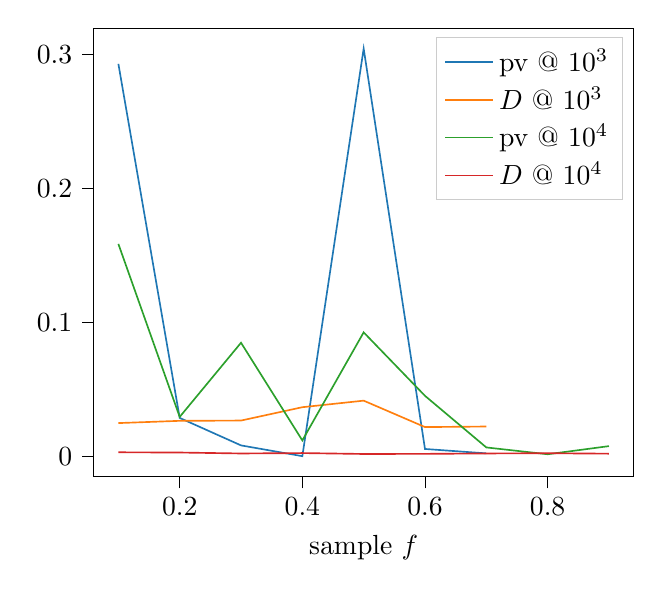
\begin{tikzpicture}

\definecolor{color0}{rgb}{0.12156862745098,0.466666666666667,0.705882352941177}
\definecolor{color1}{rgb}{1,0.498039215686275,0.0549019607843137}
\definecolor{color2}{rgb}{0.172549019607843,0.627450980392157,0.172549019607843}
\definecolor{color3}{rgb}{0.83921568627451,0.152941176470588,0.156862745098039}

\begin{axis}[
legend cell align={left},
legend style={fill opacity=0.8, draw opacity=1, text opacity=1, draw=white!80!black},
tick align=outside,
tick pos=left,
x grid style={white!69.0196078431373!black},
xlabel={sample \(\displaystyle f\)},
xmin=0.06, xmax=0.94,
xtick style={color=black},
y grid style={white!69.0196078431373!black},
ymin=-0.0152050803290124, ymax=0.319466303114614,
ytick style={color=black}
]
\addplot [semithick, color0]
table {%
0.1 0.292875492136501
0.2 0.0285593845542995
0.3 0.00804453992536252
0.4 7.25528206154844e-06
0.5 0.304253967503541
0.6 0.00538102053076603
0.7 0.00210206080073504
};
\addlegendentry{pv @ $10^3$}
\addplot [semithick, color1]
table {%
0.1 0.0247031880323107
0.2 0.0263882906142677
0.3 0.0265928795022098
0.4 0.0365549664735983
0.5 0.0414478012792164
0.6 0.0217278425900647
0.7 0.0221333226634796
};
\addlegendentry{$D$ @ $10^3$}
\addplot [semithick, color2]
table {%
0.1 0.158448404892969
0.2 0.0293173197168622
0.3 0.0846780011901316
0.4 0.0117644754543298
0.5 0.0924332279604609
0.6 0.0450527612122749
0.7 0.00653295612737991
0.8 0.00143153174844983
0.9 0.00750565939594432
};
\addlegendentry{pv @ $10^4$}
\addplot [semithick, color3]
table {%
0.1 0.00289146197840939
0.2 0.00272460611420244
0.3 0.00201659381494579
0.4 0.00231827938586626
0.5 0.00164034312801586
0.6 0.00172435367746016
0.7 0.00203139300566368
0.8 0.00219631652801155
0.9 0.001863704048015
};
\addlegendentry{$D$ @ $10^4$}
\end{axis}

\end{tikzpicture}

	\end{adjustbox}

}\caption{Olken sample}
\end{figure}
\begin{figure}
\subfloat[Sample distribution $n=10^{4}$ with $f=0.5$.\label{fig:Hash-join-1}]{    \centering
    \begin{adjustbox}{width=\linewidth,center}
    	% This file was created by tikzplotlib v0.9.8.
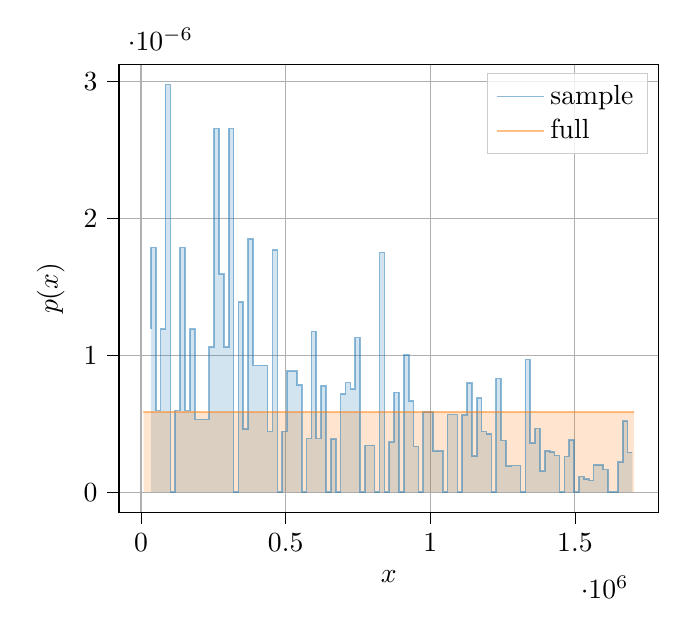
\begin{tikzpicture}

\definecolor{color0}{rgb}{0.12156862745098,0.466666666666667,0.705882352941177}
\definecolor{color1}{rgb}{1,0.498039215686275,0.0549019607843137}

\begin{axis}[
legend cell align={left},
legend style={fill opacity=0.8, draw opacity=1, text opacity=1, draw=white!80!black},
tick align=outside,
tick pos=left,
trim axis left,trim axis right,
x grid style={white!69.0196078431373!black},
xmajorgrids,
xmin=-76238.824, xmax=1789470.824,
xtick style={color=black},
xlabel={\(\displaystyle x\)},
ylabel={\(\displaystyle p(x)\)},
y grid style={white!69.0196078431373!black},
ymajorgrids,
ymin=-1.48861289495939e-07, ymax=3.12608707941472e-06,
ytick style={color=black},
ylabel near ticks
]
\path [fill=color0, fill opacity=0.2]
(axis cs:34073.29,0)
--(axis cs:34073.29,1.19089031596751e-06)
--(axis cs:34073.29,1.78633547395127e-06)
--(axis cs:50889.87,1.78633547395127e-06)
--(axis cs:50889.87,5.95445157983755e-07)
--(axis cs:67706.45,5.95445157983755e-07)
--(axis cs:67706.45,1.19089031596751e-06)
--(axis cs:84523.03,1.19089031596751e-06)
--(axis cs:84523.03,2.97722578991878e-06)
--(axis cs:101339.61,2.97722578991878e-06)
--(axis cs:101339.61,0)
--(axis cs:118156.19,0)
--(axis cs:118156.19,5.95445157983756e-07)
--(axis cs:134972.77,5.95445157983756e-07)
--(axis cs:134972.77,1.78633547395126e-06)
--(axis cs:151789.35,1.78633547395126e-06)
--(axis cs:151789.35,5.95445157983755e-07)
--(axis cs:168605.93,5.95445157983755e-07)
--(axis cs:168605.93,1.19089031596751e-06)
--(axis cs:185422.51,1.19089031596751e-06)
--(axis cs:185422.51,5.31109704132637e-07)
--(axis cs:202239.09,5.31109704132637e-07)
--(axis cs:202239.09,5.31109704132636e-07)
--(axis cs:219055.67,5.31109704132636e-07)
--(axis cs:219055.67,5.31109704132636e-07)
--(axis cs:235872.25,5.31109704132636e-07)
--(axis cs:235872.25,1.06221940826527e-06)
--(axis cs:252688.83,1.06221940826527e-06)
--(axis cs:252688.83,2.65554852066319e-06)
--(axis cs:269505.41,2.65554852066319e-06)
--(axis cs:269505.41,1.59332911239791e-06)
--(axis cs:286321.99,1.59332911239791e-06)
--(axis cs:286321.99,1.06221940826527e-06)
--(axis cs:303138.57,1.06221940826527e-06)
--(axis cs:303138.57,2.65554852066318e-06)
--(axis cs:319955.15,2.65554852066318e-06)
--(axis cs:319955.15,0)
--(axis cs:336771.73,0)
--(axis cs:336771.73,1.38800319585179e-06)
--(axis cs:353588.31,1.38800319585179e-06)
--(axis cs:353588.31,4.62667731950596e-07)
--(axis cs:370404.89,4.62667731950596e-07)
--(axis cs:370404.89,1.85067092780239e-06)
--(axis cs:387221.47,1.85067092780239e-06)
--(axis cs:387221.47,9.25335463901191e-07)
--(axis cs:404038.05,9.25335463901191e-07)
--(axis cs:404038.05,9.25335463901191e-07)
--(axis cs:420854.63,9.25335463901191e-07)
--(axis cs:420854.63,9.25335463901191e-07)
--(axis cs:437671.21,9.25335463901191e-07)
--(axis cs:437671.21,4.42135140295983e-07)
--(axis cs:454487.79,4.42135140295983e-07)
--(axis cs:454487.79,1.76854056118394e-06)
--(axis cs:471304.37,1.76854056118394e-06)
--(axis cs:471304.37,0)
--(axis cs:488120.95,0)
--(axis cs:488120.95,4.42135140295983e-07)
--(axis cs:504937.53,4.42135140295983e-07)
--(axis cs:504937.53,8.8427028059197e-07)
--(axis cs:521754.11,8.8427028059197e-07)
--(axis cs:521754.11,8.8427028059197e-07)
--(axis cs:538570.69,8.8427028059197e-07)
--(axis cs:538570.69,7.82976161762544e-07)
--(axis cs:555387.27,7.82976161762544e-07)
--(axis cs:555387.27,0)
--(axis cs:572203.85,0)
--(axis cs:572203.85,3.91488080881272e-07)
--(axis cs:589020.43,3.91488080881272e-07)
--(axis cs:589020.43,1.17446424264382e-06)
--(axis cs:605837.01,1.17446424264382e-06)
--(axis cs:605837.01,3.91488080881272e-07)
--(axis cs:622653.59,3.91488080881272e-07)
--(axis cs:622653.59,7.74763125100704e-07)
--(axis cs:639470.17,7.74763125100704e-07)
--(axis cs:639470.17,0)
--(axis cs:656286.75,0)
--(axis cs:656286.75,3.8738156255035e-07)
--(axis cs:673103.33,3.8738156255035e-07)
--(axis cs:673103.33,0)
--(axis cs:689919.91,0)
--(axis cs:689919.91,7.15903029024149e-07)
--(axis cs:706736.49,7.15903029024149e-07)
--(axis cs:706736.49,8.00771074529875e-07)
--(axis cs:723553.07,8.00771074529875e-07)
--(axis cs:723553.07,7.52861694002451e-07)
--(axis cs:740369.65,7.52861694002451e-07)
--(axis cs:740369.65,1.12929254100368e-06)
--(axis cs:757186.23,1.12929254100368e-06)
--(axis cs:757186.23,0)
--(axis cs:774002.81,0)
--(axis cs:774002.81,3.40841021466564e-07)
--(axis cs:790819.39,3.40841021466564e-07)
--(axis cs:790819.39,3.40841021466562e-07)
--(axis cs:807635.97,3.40841021466562e-07)
--(axis cs:807635.97,0)
--(axis cs:824452.55,0)
--(axis cs:824452.55,1.75074564841661e-06)
--(axis cs:841269.13,1.75074564841661e-06)
--(axis cs:841269.13,0)
--(axis cs:858085.71,0)
--(axis cs:858085.71,3.64111292008458e-07)
--(axis cs:874902.29,3.64111292008458e-07)
--(axis cs:874902.29,7.28222584016911e-07)
--(axis cs:891718.87,7.28222584016911e-07)
--(axis cs:891718.87,0)
--(axis cs:908535.45,0)
--(axis cs:908535.45,1.00199047274508e-06)
--(axis cs:925352.03,1.00199047274508e-06)
--(axis cs:925352.03,6.67993648496716e-07)
--(axis cs:942168.61,6.67993648496716e-07)
--(axis cs:942168.61,3.3399682424836e-07)
--(axis cs:958985.19,3.3399682424836e-07)
--(axis cs:958985.19,0)
--(axis cs:975801.77,0)
--(axis cs:975801.77,5.85863281878267e-07)
--(axis cs:992618.35,5.85863281878267e-07)
--(axis cs:992618.35,5.85863281878271e-07)
--(axis cs:1009434.93,5.85863281878271e-07)
--(axis cs:1009434.93,3.0114467760098e-07)
--(axis cs:1026251.51,3.0114467760098e-07)
--(axis cs:1026251.51,3.01144677600978e-07)
--(axis cs:1043068.09,3.01144677600978e-07)
--(axis cs:1043068.09,0)
--(axis cs:1059884.67,0)
--(axis cs:1059884.67,5.66699529667296e-07)
--(axis cs:1076701.25,5.66699529667296e-07)
--(axis cs:1076701.25,5.66699529667296e-07)
--(axis cs:1093517.83,5.66699529667296e-07)
--(axis cs:1093517.83,0)
--(axis cs:1110334.41,0)
--(axis cs:1110334.41,5.6122417189274e-07)
--(axis cs:1127150.99,5.6122417189274e-07)
--(axis cs:1127150.99,7.96664556198952e-07)
--(axis cs:1143967.57,7.96664556198952e-07)
--(axis cs:1143967.57,2.65554852066317e-07)
--(axis cs:1160784.15,2.65554852066317e-07)
--(axis cs:1160784.15,6.85788561264056e-07)
--(axis cs:1177600.73,6.85788561264056e-07)
--(axis cs:1177600.73,4.42135140295982e-07)
--(axis cs:1194417.31,4.42135140295982e-07)
--(axis cs:1194417.31,4.27077906415933e-07)
--(axis cs:1211233.89,4.27077906415933e-07)
--(axis cs:1211233.89,0)
--(axis cs:1228050.47,0)
--(axis cs:1228050.47,8.30885542289984e-07)
--(axis cs:1244867.05,8.30885542289984e-07)
--(axis cs:1244867.05,3.77799686444864e-07)
--(axis cs:1261683.63,3.77799686444864e-07)
--(axis cs:1261683.63,1.88899843222432e-07)
--(axis cs:1278500.21,1.88899843222432e-07)
--(axis cs:1278500.21,1.94375200996998e-07)
--(axis cs:1295316.79,1.94375200996998e-07)
--(axis cs:1295316.79,1.94375200996995e-07)
--(axis cs:1312133.37,1.94375200996995e-07)
--(axis cs:1312133.37,0)
--(axis cs:1328949.95,0)
--(axis cs:1328949.95,9.69138326097708e-07)
--(axis cs:1345766.53,9.69138326097708e-07)
--(axis cs:1345766.53,3.61373613121174e-07)
--(axis cs:1362583.11,3.61373613121174e-07)
--(axis cs:1362583.11,4.64036571394235e-07)
--(axis cs:1379399.69,4.64036571394235e-07)
--(axis cs:1379399.69,1.53310017687773e-07)
--(axis cs:1396216.27,1.53310017687773e-07)
--(axis cs:1396216.27,2.99775838157338e-07)
--(axis cs:1413032.85,2.99775838157338e-07)
--(axis cs:1413032.85,2.94300480382774e-07)
--(axis cs:1429849.43,2.94300480382774e-07)
--(axis cs:1429849.43,2.68292530953603e-07)
--(axis cs:1446666.01,2.68292530953603e-07)
--(axis cs:1446666.01,0)
--(axis cs:1463482.59,0)
--(axis cs:1463482.59,2.60079494291754e-07)
--(axis cs:1480299.17,2.60079494291754e-07)
--(axis cs:1480299.17,3.7916852588851e-07)
--(axis cs:1497115.75,3.7916852588851e-07)
--(axis cs:1497115.75,0)
--(axis cs:1513932.33,0)
--(axis cs:1513932.33,1.13613673822187e-07)
--(axis cs:1530748.91,1.13613673822187e-07)
--(axis cs:1530748.91,9.4449921611216e-08)
--(axis cs:1547565.49,9.4449921611216e-08)
--(axis cs:1547565.49,8.62368849493723e-08)
--(axis cs:1564382.07,8.62368849493723e-08)
--(axis cs:1564382.07,1.99850558771558e-07)
--(axis cs:1581198.65,1.99850558771558e-07)
--(axis cs:1581198.65,1.97112879884277e-07)
--(axis cs:1598015.23,1.97112879884277e-07)
--(axis cs:1598015.23,1.642607332369e-07)
--(axis cs:1614831.81,1.642607332369e-07)
--(axis cs:1614831.81,0)
--(axis cs:1631648.39,0)
--(axis cs:1631648.39,0)
--(axis cs:1648464.97,0)
--(axis cs:1648464.97,2.19014310982533e-07)
--(axis cs:1665281.55,2.19014310982533e-07)
--(axis cs:1665281.55,5.18790149139867e-07)
--(axis cs:1682098.13,5.18790149139867e-07)
--(axis cs:1682098.13,2.90193962051856e-07)
--(axis cs:1698914.71,2.90193962051856e-07)
--(axis cs:1698914.71,0)
--(axis cs:1698914.71,0)
--(axis cs:1682098.13,0)
--(axis cs:1682098.13,0)
--(axis cs:1665281.55,0)
--(axis cs:1665281.55,0)
--(axis cs:1648464.97,0)
--(axis cs:1648464.97,0)
--(axis cs:1631648.39,0)
--(axis cs:1631648.39,0)
--(axis cs:1614831.81,0)
--(axis cs:1614831.81,0)
--(axis cs:1598015.23,0)
--(axis cs:1598015.23,0)
--(axis cs:1581198.65,0)
--(axis cs:1581198.65,0)
--(axis cs:1564382.07,0)
--(axis cs:1564382.07,0)
--(axis cs:1547565.49,0)
--(axis cs:1547565.49,0)
--(axis cs:1530748.91,0)
--(axis cs:1530748.91,0)
--(axis cs:1513932.33,0)
--(axis cs:1513932.33,0)
--(axis cs:1497115.75,0)
--(axis cs:1497115.75,0)
--(axis cs:1480299.17,0)
--(axis cs:1480299.17,0)
--(axis cs:1463482.59,0)
--(axis cs:1463482.59,0)
--(axis cs:1446666.01,0)
--(axis cs:1446666.01,0)
--(axis cs:1429849.43,0)
--(axis cs:1429849.43,0)
--(axis cs:1413032.85,0)
--(axis cs:1413032.85,0)
--(axis cs:1396216.27,0)
--(axis cs:1396216.27,0)
--(axis cs:1379399.69,0)
--(axis cs:1379399.69,0)
--(axis cs:1362583.11,0)
--(axis cs:1362583.11,0)
--(axis cs:1345766.53,0)
--(axis cs:1345766.53,0)
--(axis cs:1328949.95,0)
--(axis cs:1328949.95,0)
--(axis cs:1312133.37,0)
--(axis cs:1312133.37,0)
--(axis cs:1295316.79,0)
--(axis cs:1295316.79,0)
--(axis cs:1278500.21,0)
--(axis cs:1278500.21,0)
--(axis cs:1261683.63,0)
--(axis cs:1261683.63,0)
--(axis cs:1244867.05,0)
--(axis cs:1244867.05,0)
--(axis cs:1228050.47,0)
--(axis cs:1228050.47,0)
--(axis cs:1211233.89,0)
--(axis cs:1211233.89,0)
--(axis cs:1194417.31,0)
--(axis cs:1194417.31,0)
--(axis cs:1177600.73,0)
--(axis cs:1177600.73,0)
--(axis cs:1160784.15,0)
--(axis cs:1160784.15,0)
--(axis cs:1143967.57,0)
--(axis cs:1143967.57,0)
--(axis cs:1127150.99,0)
--(axis cs:1127150.99,0)
--(axis cs:1110334.41,0)
--(axis cs:1110334.41,0)
--(axis cs:1093517.83,0)
--(axis cs:1093517.83,0)
--(axis cs:1076701.25,0)
--(axis cs:1076701.25,0)
--(axis cs:1059884.67,0)
--(axis cs:1059884.67,0)
--(axis cs:1043068.09,0)
--(axis cs:1043068.09,0)
--(axis cs:1026251.51,0)
--(axis cs:1026251.51,0)
--(axis cs:1009434.93,0)
--(axis cs:1009434.93,0)
--(axis cs:992618.35,0)
--(axis cs:992618.35,0)
--(axis cs:975801.77,0)
--(axis cs:975801.77,0)
--(axis cs:958985.19,0)
--(axis cs:958985.19,0)
--(axis cs:942168.61,0)
--(axis cs:942168.61,0)
--(axis cs:925352.03,0)
--(axis cs:925352.03,0)
--(axis cs:908535.45,0)
--(axis cs:908535.45,0)
--(axis cs:891718.87,0)
--(axis cs:891718.87,0)
--(axis cs:874902.29,0)
--(axis cs:874902.29,0)
--(axis cs:858085.71,0)
--(axis cs:858085.71,0)
--(axis cs:841269.13,0)
--(axis cs:841269.13,0)
--(axis cs:824452.55,0)
--(axis cs:824452.55,0)
--(axis cs:807635.97,0)
--(axis cs:807635.97,0)
--(axis cs:790819.39,0)
--(axis cs:790819.39,0)
--(axis cs:774002.81,0)
--(axis cs:774002.81,0)
--(axis cs:757186.23,0)
--(axis cs:757186.23,0)
--(axis cs:740369.65,0)
--(axis cs:740369.65,0)
--(axis cs:723553.07,0)
--(axis cs:723553.07,0)
--(axis cs:706736.49,0)
--(axis cs:706736.49,0)
--(axis cs:689919.91,0)
--(axis cs:689919.91,0)
--(axis cs:673103.33,0)
--(axis cs:673103.33,0)
--(axis cs:656286.75,0)
--(axis cs:656286.75,0)
--(axis cs:639470.17,0)
--(axis cs:639470.17,0)
--(axis cs:622653.59,0)
--(axis cs:622653.59,0)
--(axis cs:605837.01,0)
--(axis cs:605837.01,0)
--(axis cs:589020.43,0)
--(axis cs:589020.43,0)
--(axis cs:572203.85,0)
--(axis cs:572203.85,0)
--(axis cs:555387.27,0)
--(axis cs:555387.27,0)
--(axis cs:538570.69,0)
--(axis cs:538570.69,0)
--(axis cs:521754.11,0)
--(axis cs:521754.11,0)
--(axis cs:504937.53,0)
--(axis cs:504937.53,0)
--(axis cs:488120.95,0)
--(axis cs:488120.95,0)
--(axis cs:471304.37,0)
--(axis cs:471304.37,0)
--(axis cs:454487.79,0)
--(axis cs:454487.79,0)
--(axis cs:437671.21,0)
--(axis cs:437671.21,0)
--(axis cs:420854.63,0)
--(axis cs:420854.63,0)
--(axis cs:404038.05,0)
--(axis cs:404038.05,0)
--(axis cs:387221.47,0)
--(axis cs:387221.47,0)
--(axis cs:370404.89,0)
--(axis cs:370404.89,0)
--(axis cs:353588.31,0)
--(axis cs:353588.31,0)
--(axis cs:336771.73,0)
--(axis cs:336771.73,0)
--(axis cs:319955.15,0)
--(axis cs:319955.15,0)
--(axis cs:303138.57,0)
--(axis cs:303138.57,0)
--(axis cs:286321.99,0)
--(axis cs:286321.99,0)
--(axis cs:269505.41,0)
--(axis cs:269505.41,0)
--(axis cs:252688.83,0)
--(axis cs:252688.83,0)
--(axis cs:235872.25,0)
--(axis cs:235872.25,0)
--(axis cs:219055.67,0)
--(axis cs:219055.67,0)
--(axis cs:202239.09,0)
--(axis cs:202239.09,0)
--(axis cs:185422.51,0)
--(axis cs:185422.51,0)
--(axis cs:168605.93,0)
--(axis cs:168605.93,0)
--(axis cs:151789.35,0)
--(axis cs:151789.35,0)
--(axis cs:134972.77,0)
--(axis cs:134972.77,0)
--(axis cs:118156.19,0)
--(axis cs:118156.19,0)
--(axis cs:101339.61,0)
--(axis cs:101339.61,0)
--(axis cs:84523.03,0)
--(axis cs:84523.03,0)
--(axis cs:67706.45,0)
--(axis cs:67706.45,0)
--(axis cs:50889.87,0)
--(axis cs:50889.87,0)
--(axis cs:34073.29,0)
--(axis cs:34073.29,0)
--cycle;

\path [fill=color1, fill opacity=0.2]
(axis cs:8566.16,0)
--(axis cs:8566.16,5.8371493606733e-07)
--(axis cs:8566.16,5.83680866439357e-07)
--(axis cs:25698.48,5.83680866439357e-07)
--(axis cs:25698.48,5.83680866439357e-07)
--(axis cs:42830.8,5.83680866439357e-07)
--(axis cs:42830.8,5.8371493606733e-07)
--(axis cs:59963.12,5.8371493606733e-07)
--(axis cs:59963.12,5.83680866439357e-07)
--(axis cs:77095.44,5.83680866439357e-07)
--(axis cs:77095.44,5.83680866439357e-07)
--(axis cs:94227.76,5.83680866439357e-07)
--(axis cs:94227.76,5.83714936067331e-07)
--(axis cs:111360.08,5.83714936067331e-07)
--(axis cs:111360.08,5.83680866439357e-07)
--(axis cs:128492.4,5.83680866439357e-07)
--(axis cs:128492.4,5.83680866439357e-07)
--(axis cs:145624.72,5.83680866439357e-07)
--(axis cs:145624.72,5.8371493606733e-07)
--(axis cs:162757.04,5.8371493606733e-07)
--(axis cs:162757.04,5.83680866439358e-07)
--(axis cs:179889.36,5.83680866439358e-07)
--(axis cs:179889.36,5.83680866439357e-07)
--(axis cs:197021.68,5.83680866439357e-07)
--(axis cs:197021.68,5.8371493606733e-07)
--(axis cs:214154,5.8371493606733e-07)
--(axis cs:214154,5.83680866439358e-07)
--(axis cs:231286.32,5.83680866439358e-07)
--(axis cs:231286.32,5.83680866439357e-07)
--(axis cs:248418.64,5.83680866439357e-07)
--(axis cs:248418.64,5.8371493606733e-07)
--(axis cs:265550.96,5.8371493606733e-07)
--(axis cs:265550.96,5.83680866439357e-07)
--(axis cs:282683.28,5.83680866439357e-07)
--(axis cs:282683.28,5.83680866439357e-07)
--(axis cs:299815.6,5.83680866439357e-07)
--(axis cs:299815.6,5.8371493606733e-07)
--(axis cs:316947.92,5.8371493606733e-07)
--(axis cs:316947.92,5.83680866439357e-07)
--(axis cs:334080.24,5.83680866439357e-07)
--(axis cs:334080.24,5.83680866439359e-07)
--(axis cs:351212.56,5.83680866439359e-07)
--(axis cs:351212.56,5.8371493606733e-07)
--(axis cs:368344.88,5.8371493606733e-07)
--(axis cs:368344.88,5.83680866439357e-07)
--(axis cs:385477.2,5.83680866439357e-07)
--(axis cs:385477.2,5.83680866439357e-07)
--(axis cs:402609.52,5.83680866439357e-07)
--(axis cs:402609.52,5.83680866439357e-07)
--(axis cs:419741.84,5.83680866439357e-07)
--(axis cs:419741.84,5.8371493606733e-07)
--(axis cs:436874.16,5.8371493606733e-07)
--(axis cs:436874.16,5.83680866439357e-07)
--(axis cs:454006.48,5.83680866439357e-07)
--(axis cs:454006.48,5.83680866439359e-07)
--(axis cs:471138.8,5.83680866439359e-07)
--(axis cs:471138.8,5.8371493606733e-07)
--(axis cs:488271.12,5.8371493606733e-07)
--(axis cs:488271.12,5.83680866439357e-07)
--(axis cs:505403.44,5.83680866439357e-07)
--(axis cs:505403.44,5.83680866439355e-07)
--(axis cs:522535.76,5.83680866439355e-07)
--(axis cs:522535.76,5.83714936067332e-07)
--(axis cs:539668.08,5.83714936067332e-07)
--(axis cs:539668.08,5.83680866439359e-07)
--(axis cs:556800.4,5.83680866439359e-07)
--(axis cs:556800.4,5.83680866439355e-07)
--(axis cs:573932.72,5.83680866439355e-07)
--(axis cs:573932.72,5.83714936067332e-07)
--(axis cs:591065.04,5.83714936067332e-07)
--(axis cs:591065.04,5.83680866439355e-07)
--(axis cs:608197.36,5.83680866439355e-07)
--(axis cs:608197.36,5.83680866439359e-07)
--(axis cs:625329.68,5.83680866439359e-07)
--(axis cs:625329.68,5.83714936067328e-07)
--(axis cs:642462,5.83714936067328e-07)
--(axis cs:642462,5.83680866439359e-07)
--(axis cs:659594.32,5.83680866439359e-07)
--(axis cs:659594.32,5.83680866439355e-07)
--(axis cs:676726.64,5.83680866439355e-07)
--(axis cs:676726.64,5.83714936067332e-07)
--(axis cs:693858.96,5.83714936067332e-07)
--(axis cs:693858.96,5.83680866439359e-07)
--(axis cs:710991.28,5.83680866439359e-07)
--(axis cs:710991.28,5.83680866439355e-07)
--(axis cs:728123.6,5.83680866439355e-07)
--(axis cs:728123.6,5.83714936067332e-07)
--(axis cs:745255.92,5.83714936067332e-07)
--(axis cs:745255.92,5.83680866439355e-07)
--(axis cs:762388.24,5.83680866439355e-07)
--(axis cs:762388.24,5.83680866439359e-07)
--(axis cs:779520.56,5.83680866439359e-07)
--(axis cs:779520.56,5.83714936067328e-07)
--(axis cs:796652.88,5.83714936067328e-07)
--(axis cs:796652.88,5.83680866439359e-07)
--(axis cs:813785.2,5.83680866439359e-07)
--(axis cs:813785.2,5.83680866439359e-07)
--(axis cs:830917.52,5.83680866439359e-07)
--(axis cs:830917.52,5.83680866439355e-07)
--(axis cs:848049.84,5.83680866439355e-07)
--(axis cs:848049.84,5.83714936067332e-07)
--(axis cs:865182.16,5.83714936067332e-07)
--(axis cs:865182.16,5.83680866439355e-07)
--(axis cs:882314.48,5.83680866439355e-07)
--(axis cs:882314.48,5.83680866439359e-07)
--(axis cs:899446.8,5.83680866439359e-07)
--(axis cs:899446.8,5.83714936067328e-07)
--(axis cs:916579.12,5.83714936067328e-07)
--(axis cs:916579.12,5.83680866439359e-07)
--(axis cs:933711.44,5.83680866439359e-07)
--(axis cs:933711.44,5.83680866439359e-07)
--(axis cs:950843.76,5.83680866439359e-07)
--(axis cs:950843.76,5.83714936067328e-07)
--(axis cs:967976.08,5.83714936067328e-07)
--(axis cs:967976.08,5.83680866439359e-07)
--(axis cs:985108.4,5.83680866439359e-07)
--(axis cs:985108.4,5.83680866439355e-07)
--(axis cs:1002240.72,5.83680866439355e-07)
--(axis cs:1002240.72,5.83714936067332e-07)
--(axis cs:1019373.04,5.83714936067332e-07)
--(axis cs:1019373.04,5.83680866439355e-07)
--(axis cs:1036505.36,5.83680866439355e-07)
--(axis cs:1036505.36,5.83680866439355e-07)
--(axis cs:1053637.68,5.83680866439355e-07)
--(axis cs:1053637.68,5.83714936067336e-07)
--(axis cs:1070770,5.83714936067336e-07)
--(axis cs:1070770,5.83680866439355e-07)
--(axis cs:1087902.32,5.83680866439355e-07)
--(axis cs:1087902.32,5.83680866439355e-07)
--(axis cs:1105034.64,5.83680866439355e-07)
--(axis cs:1105034.64,5.83714936067336e-07)
--(axis cs:1122166.96,5.83714936067336e-07)
--(axis cs:1122166.96,5.83680866439355e-07)
--(axis cs:1139299.28,5.83680866439355e-07)
--(axis cs:1139299.28,5.83680866439355e-07)
--(axis cs:1156431.6,5.83680866439355e-07)
--(axis cs:1156431.6,5.83714936067328e-07)
--(axis cs:1173563.92,5.83714936067328e-07)
--(axis cs:1173563.92,5.83680866439363e-07)
--(axis cs:1190696.24,5.83680866439363e-07)
--(axis cs:1190696.24,5.83680866439355e-07)
--(axis cs:1207828.56,5.83680866439355e-07)
--(axis cs:1207828.56,5.83714936067328e-07)
--(axis cs:1224960.88,5.83714936067328e-07)
--(axis cs:1224960.88,5.83680866439363e-07)
--(axis cs:1242093.2,5.83680866439363e-07)
--(axis cs:1242093.2,5.83680866439355e-07)
--(axis cs:1259225.52,5.83680866439355e-07)
--(axis cs:1259225.52,5.83680866439355e-07)
--(axis cs:1276357.84,5.83680866439355e-07)
--(axis cs:1276357.84,5.83714936067328e-07)
--(axis cs:1293490.16,5.83714936067328e-07)
--(axis cs:1293490.16,5.83680866439363e-07)
--(axis cs:1310622.48,5.83680866439363e-07)
--(axis cs:1310622.48,5.83680866439355e-07)
--(axis cs:1327754.8,5.83680866439355e-07)
--(axis cs:1327754.8,5.83714936067328e-07)
--(axis cs:1344887.12,5.83714936067328e-07)
--(axis cs:1344887.12,5.83680866439355e-07)
--(axis cs:1362019.44,5.83680866439355e-07)
--(axis cs:1362019.44,5.83680866439363e-07)
--(axis cs:1379151.76,5.83680866439363e-07)
--(axis cs:1379151.76,5.83714936067328e-07)
--(axis cs:1396284.08,5.83714936067328e-07)
--(axis cs:1396284.08,5.83680866439355e-07)
--(axis cs:1413416.4,5.83680866439355e-07)
--(axis cs:1413416.4,5.83680866439363e-07)
--(axis cs:1430548.72,5.83680866439363e-07)
--(axis cs:1430548.72,5.83714936067328e-07)
--(axis cs:1447681.04,5.83714936067328e-07)
--(axis cs:1447681.04,5.83680866439355e-07)
--(axis cs:1464813.36,5.83680866439355e-07)
--(axis cs:1464813.36,5.83680866439355e-07)
--(axis cs:1481945.68,5.83680866439355e-07)
--(axis cs:1481945.68,5.83714936067336e-07)
--(axis cs:1499078,5.83714936067336e-07)
--(axis cs:1499078,5.83680866439355e-07)
--(axis cs:1516210.32,5.83680866439355e-07)
--(axis cs:1516210.32,5.83680866439355e-07)
--(axis cs:1533342.64,5.83680866439355e-07)
--(axis cs:1533342.64,5.83714936067336e-07)
--(axis cs:1550474.96,5.83714936067336e-07)
--(axis cs:1550474.96,5.83680866439355e-07)
--(axis cs:1567607.28,5.83680866439355e-07)
--(axis cs:1567607.28,5.83680866439355e-07)
--(axis cs:1584739.6,5.83680866439355e-07)
--(axis cs:1584739.6,5.83714936067328e-07)
--(axis cs:1601871.92,5.83714936067328e-07)
--(axis cs:1601871.92,5.83680866439363e-07)
--(axis cs:1619004.24,5.83680866439363e-07)
--(axis cs:1619004.24,5.83680866439355e-07)
--(axis cs:1636136.56,5.83680866439355e-07)
--(axis cs:1636136.56,5.83714936067328e-07)
--(axis cs:1653268.88,5.83714936067328e-07)
--(axis cs:1653268.88,5.83680866439363e-07)
--(axis cs:1670401.2,5.83680866439363e-07)
--(axis cs:1670401.2,5.83680866439355e-07)
--(axis cs:1687533.52,5.83680866439355e-07)
--(axis cs:1687533.52,5.83714936067328e-07)
--(axis cs:1704665.84,5.83714936067328e-07)
--(axis cs:1704665.84,0)
--(axis cs:1704665.84,0)
--(axis cs:1687533.52,0)
--(axis cs:1687533.52,0)
--(axis cs:1670401.2,0)
--(axis cs:1670401.2,0)
--(axis cs:1653268.88,0)
--(axis cs:1653268.88,0)
--(axis cs:1636136.56,0)
--(axis cs:1636136.56,0)
--(axis cs:1619004.24,0)
--(axis cs:1619004.24,0)
--(axis cs:1601871.92,0)
--(axis cs:1601871.92,0)
--(axis cs:1584739.6,0)
--(axis cs:1584739.6,0)
--(axis cs:1567607.28,0)
--(axis cs:1567607.28,0)
--(axis cs:1550474.96,0)
--(axis cs:1550474.96,0)
--(axis cs:1533342.64,0)
--(axis cs:1533342.64,0)
--(axis cs:1516210.32,0)
--(axis cs:1516210.32,0)
--(axis cs:1499078,0)
--(axis cs:1499078,0)
--(axis cs:1481945.68,0)
--(axis cs:1481945.68,0)
--(axis cs:1464813.36,0)
--(axis cs:1464813.36,0)
--(axis cs:1447681.04,0)
--(axis cs:1447681.04,0)
--(axis cs:1430548.72,0)
--(axis cs:1430548.72,0)
--(axis cs:1413416.4,0)
--(axis cs:1413416.4,0)
--(axis cs:1396284.08,0)
--(axis cs:1396284.08,0)
--(axis cs:1379151.76,0)
--(axis cs:1379151.76,0)
--(axis cs:1362019.44,0)
--(axis cs:1362019.44,0)
--(axis cs:1344887.12,0)
--(axis cs:1344887.12,0)
--(axis cs:1327754.8,0)
--(axis cs:1327754.8,0)
--(axis cs:1310622.48,0)
--(axis cs:1310622.48,0)
--(axis cs:1293490.16,0)
--(axis cs:1293490.16,0)
--(axis cs:1276357.84,0)
--(axis cs:1276357.84,0)
--(axis cs:1259225.52,0)
--(axis cs:1259225.52,0)
--(axis cs:1242093.2,0)
--(axis cs:1242093.2,0)
--(axis cs:1224960.88,0)
--(axis cs:1224960.88,0)
--(axis cs:1207828.56,0)
--(axis cs:1207828.56,0)
--(axis cs:1190696.24,0)
--(axis cs:1190696.24,0)
--(axis cs:1173563.92,0)
--(axis cs:1173563.92,0)
--(axis cs:1156431.6,0)
--(axis cs:1156431.6,0)
--(axis cs:1139299.28,0)
--(axis cs:1139299.28,0)
--(axis cs:1122166.96,0)
--(axis cs:1122166.96,0)
--(axis cs:1105034.64,0)
--(axis cs:1105034.64,0)
--(axis cs:1087902.32,0)
--(axis cs:1087902.32,0)
--(axis cs:1070770,0)
--(axis cs:1070770,0)
--(axis cs:1053637.68,0)
--(axis cs:1053637.68,0)
--(axis cs:1036505.36,0)
--(axis cs:1036505.36,0)
--(axis cs:1019373.04,0)
--(axis cs:1019373.04,0)
--(axis cs:1002240.72,0)
--(axis cs:1002240.72,0)
--(axis cs:985108.4,0)
--(axis cs:985108.4,0)
--(axis cs:967976.08,0)
--(axis cs:967976.08,0)
--(axis cs:950843.76,0)
--(axis cs:950843.76,0)
--(axis cs:933711.44,0)
--(axis cs:933711.44,0)
--(axis cs:916579.12,0)
--(axis cs:916579.12,0)
--(axis cs:899446.8,0)
--(axis cs:899446.8,0)
--(axis cs:882314.48,0)
--(axis cs:882314.48,0)
--(axis cs:865182.16,0)
--(axis cs:865182.16,0)
--(axis cs:848049.84,0)
--(axis cs:848049.84,0)
--(axis cs:830917.52,0)
--(axis cs:830917.52,0)
--(axis cs:813785.2,0)
--(axis cs:813785.2,0)
--(axis cs:796652.88,0)
--(axis cs:796652.88,0)
--(axis cs:779520.56,0)
--(axis cs:779520.56,0)
--(axis cs:762388.24,0)
--(axis cs:762388.24,0)
--(axis cs:745255.92,0)
--(axis cs:745255.92,0)
--(axis cs:728123.6,0)
--(axis cs:728123.6,0)
--(axis cs:710991.28,0)
--(axis cs:710991.28,0)
--(axis cs:693858.96,0)
--(axis cs:693858.96,0)
--(axis cs:676726.64,0)
--(axis cs:676726.64,0)
--(axis cs:659594.32,0)
--(axis cs:659594.32,0)
--(axis cs:642462,0)
--(axis cs:642462,0)
--(axis cs:625329.68,0)
--(axis cs:625329.68,0)
--(axis cs:608197.36,0)
--(axis cs:608197.36,0)
--(axis cs:591065.04,0)
--(axis cs:591065.04,0)
--(axis cs:573932.72,0)
--(axis cs:573932.72,0)
--(axis cs:556800.4,0)
--(axis cs:556800.4,0)
--(axis cs:539668.08,0)
--(axis cs:539668.08,0)
--(axis cs:522535.76,0)
--(axis cs:522535.76,0)
--(axis cs:505403.44,0)
--(axis cs:505403.44,0)
--(axis cs:488271.12,0)
--(axis cs:488271.12,0)
--(axis cs:471138.8,0)
--(axis cs:471138.8,0)
--(axis cs:454006.48,0)
--(axis cs:454006.48,0)
--(axis cs:436874.16,0)
--(axis cs:436874.16,0)
--(axis cs:419741.84,0)
--(axis cs:419741.84,0)
--(axis cs:402609.52,0)
--(axis cs:402609.52,0)
--(axis cs:385477.2,0)
--(axis cs:385477.2,0)
--(axis cs:368344.88,0)
--(axis cs:368344.88,0)
--(axis cs:351212.56,0)
--(axis cs:351212.56,0)
--(axis cs:334080.24,0)
--(axis cs:334080.24,0)
--(axis cs:316947.92,0)
--(axis cs:316947.92,0)
--(axis cs:299815.6,0)
--(axis cs:299815.6,0)
--(axis cs:282683.28,0)
--(axis cs:282683.28,0)
--(axis cs:265550.96,0)
--(axis cs:265550.96,0)
--(axis cs:248418.64,0)
--(axis cs:248418.64,0)
--(axis cs:231286.32,0)
--(axis cs:231286.32,0)
--(axis cs:214154,0)
--(axis cs:214154,0)
--(axis cs:197021.68,0)
--(axis cs:197021.68,0)
--(axis cs:179889.36,0)
--(axis cs:179889.36,0)
--(axis cs:162757.04,0)
--(axis cs:162757.04,0)
--(axis cs:145624.72,0)
--(axis cs:145624.72,0)
--(axis cs:128492.4,0)
--(axis cs:128492.4,0)
--(axis cs:111360.08,0)
--(axis cs:111360.08,0)
--(axis cs:94227.76,0)
--(axis cs:94227.76,0)
--(axis cs:77095.44,0)
--(axis cs:77095.44,0)
--(axis cs:59963.12,0)
--(axis cs:59963.12,0)
--(axis cs:42830.8,0)
--(axis cs:42830.8,0)
--(axis cs:25698.48,0)
--(axis cs:25698.48,0)
--(axis cs:8566.16,0)
--(axis cs:8566.16,0)
--cycle;

\addplot [semithick, color0, const plot mark right, opacity=0.5]
table {%
34073.29 1.19089031596751e-06
50889.87 1.78633547395127e-06
67706.45 5.95445157983755e-07
84523.03 1.19089031596751e-06
101339.61 2.97722578991878e-06
118156.19 0
134972.77 5.95445157983756e-07
151789.35 1.78633547395126e-06
168605.93 5.95445157983755e-07
185422.51 1.19089031596751e-06
202239.09 5.31109704132637e-07
219055.67 5.31109704132636e-07
235872.25 5.31109704132636e-07
252688.83 1.06221940826527e-06
269505.41 2.65554852066319e-06
286321.99 1.59332911239791e-06
303138.57 1.06221940826527e-06
319955.15 2.65554852066318e-06
336771.73 0
353588.31 1.38800319585179e-06
370404.89 4.62667731950596e-07
387221.47 1.85067092780239e-06
404038.05 9.25335463901191e-07
420854.63 9.25335463901191e-07
437671.21 9.25335463901191e-07
454487.79 4.42135140295983e-07
471304.37 1.76854056118394e-06
488120.95 0
504937.53 4.42135140295983e-07
521754.11 8.8427028059197e-07
538570.69 8.8427028059197e-07
555387.27 7.82976161762544e-07
572203.85 0
589020.43 3.91488080881272e-07
605837.01 1.17446424264382e-06
622653.59 3.91488080881272e-07
639470.17 7.74763125100704e-07
656286.75 0
673103.33 3.8738156255035e-07
689919.91 0
706736.49 7.15903029024149e-07
723553.07 8.00771074529875e-07
740369.65 7.52861694002451e-07
757186.23 1.12929254100368e-06
774002.81 0
790819.39 3.40841021466564e-07
807635.97 3.40841021466562e-07
824452.55 0
841269.13 1.75074564841661e-06
858085.71 0
874902.29 3.64111292008458e-07
891718.87 7.28222584016911e-07
908535.45 0
925352.03 1.00199047274508e-06
942168.61 6.67993648496716e-07
958985.19 3.3399682424836e-07
975801.77 0
992618.35 5.85863281878267e-07
1009434.93 5.85863281878271e-07
1026251.51 3.0114467760098e-07
1043068.09 3.01144677600978e-07
1059884.67 0
1076701.25 5.66699529667296e-07
1093517.83 5.66699529667296e-07
1110334.41 0
1127150.99 5.6122417189274e-07
1143967.57 7.96664556198952e-07
1160784.15 2.65554852066317e-07
1177600.73 6.85788561264056e-07
1194417.31 4.42135140295982e-07
1211233.89 4.27077906415933e-07
1228050.47 0
1244867.05 8.30885542289984e-07
1261683.63 3.77799686444864e-07
1278500.21 1.88899843222432e-07
1295316.79 1.94375200996998e-07
1312133.37 1.94375200996995e-07
1328949.95 0
1345766.53 9.69138326097708e-07
1362583.11 3.61373613121174e-07
1379399.69 4.64036571394235e-07
1396216.27 1.53310017687773e-07
1413032.85 2.99775838157338e-07
1429849.43 2.94300480382774e-07
1446666.01 2.68292530953603e-07
1463482.59 0
1480299.17 2.60079494291754e-07
1497115.75 3.7916852588851e-07
1513932.33 0
1530748.91 1.13613673822187e-07
1547565.49 9.4449921611216e-08
1564382.07 8.62368849493723e-08
1581198.65 1.99850558771558e-07
1598015.23 1.97112879884277e-07
1614831.81 1.642607332369e-07
1631648.39 0
1648464.97 0
1665281.55 2.19014310982533e-07
1682098.13 5.18790149139867e-07
1698914.71 2.90193962051856e-07
};
\addlegendentry{sample}
\addplot [semithick, color1, const plot mark right, opacity=0.5]
table {%
8566.16 5.8371493606733e-07
25698.48 5.83680866439357e-07
42830.8 5.83680866439357e-07
59963.12 5.8371493606733e-07
77095.44 5.83680866439357e-07
94227.76 5.83680866439357e-07
111360.08 5.83714936067331e-07
128492.4 5.83680866439357e-07
145624.72 5.83680866439357e-07
162757.04 5.8371493606733e-07
179889.36 5.83680866439358e-07
197021.68 5.83680866439357e-07
214154 5.8371493606733e-07
231286.32 5.83680866439358e-07
248418.64 5.83680866439357e-07
265550.96 5.8371493606733e-07
282683.28 5.83680866439357e-07
299815.6 5.83680866439357e-07
316947.92 5.8371493606733e-07
334080.24 5.83680866439357e-07
351212.56 5.83680866439359e-07
368344.88 5.8371493606733e-07
385477.2 5.83680866439357e-07
402609.52 5.83680866439357e-07
419741.84 5.83680866439357e-07
436874.16 5.8371493606733e-07
454006.48 5.83680866439357e-07
471138.8 5.83680866439359e-07
488271.12 5.8371493606733e-07
505403.44 5.83680866439357e-07
522535.76 5.83680866439355e-07
539668.08 5.83714936067332e-07
556800.4 5.83680866439359e-07
573932.72 5.83680866439355e-07
591065.04 5.83714936067332e-07
608197.36 5.83680866439355e-07
625329.68 5.83680866439359e-07
642462 5.83714936067328e-07
659594.32 5.83680866439359e-07
676726.64 5.83680866439355e-07
693858.96 5.83714936067332e-07
710991.28 5.83680866439359e-07
728123.6 5.83680866439355e-07
745255.92 5.83714936067332e-07
762388.24 5.83680866439355e-07
779520.56 5.83680866439359e-07
796652.88 5.83714936067328e-07
813785.2 5.83680866439359e-07
830917.52 5.83680866439359e-07
848049.84 5.83680866439355e-07
865182.16 5.83714936067332e-07
882314.48 5.83680866439355e-07
899446.8 5.83680866439359e-07
916579.12 5.83714936067328e-07
933711.44 5.83680866439359e-07
950843.76 5.83680866439359e-07
967976.08 5.83714936067328e-07
985108.4 5.83680866439359e-07
1002240.72 5.83680866439355e-07
1019373.04 5.83714936067332e-07
1036505.36 5.83680866439355e-07
1053637.68 5.83680866439355e-07
1070770 5.83714936067336e-07
1087902.32 5.83680866439355e-07
1105034.64 5.83680866439355e-07
1122166.96 5.83714936067336e-07
1139299.28 5.83680866439355e-07
1156431.6 5.83680866439355e-07
1173563.92 5.83714936067328e-07
1190696.24 5.83680866439363e-07
1207828.56 5.83680866439355e-07
1224960.88 5.83714936067328e-07
1242093.2 5.83680866439363e-07
1259225.52 5.83680866439355e-07
1276357.84 5.83680866439355e-07
1293490.16 5.83714936067328e-07
1310622.48 5.83680866439363e-07
1327754.8 5.83680866439355e-07
1344887.12 5.83714936067328e-07
1362019.44 5.83680866439355e-07
1379151.76 5.83680866439363e-07
1396284.08 5.83714936067328e-07
1413416.4 5.83680866439355e-07
1430548.72 5.83680866439363e-07
1447681.04 5.83714936067328e-07
1464813.36 5.83680866439355e-07
1481945.68 5.83680866439355e-07
1499078 5.83714936067336e-07
1516210.32 5.83680866439355e-07
1533342.64 5.83680866439355e-07
1550474.96 5.83714936067336e-07
1567607.28 5.83680866439355e-07
1584739.6 5.83680866439355e-07
1601871.92 5.83714936067328e-07
1619004.24 5.83680866439363e-07
1636136.56 5.83680866439355e-07
1653268.88 5.83714936067328e-07
1670401.2 5.83680866439363e-07
1687533.52 5.83680866439355e-07
1704665.84 5.83714936067328e-07
};
\addlegendentry{full}
\end{axis}

\end{tikzpicture}

	\end{adjustbox}}\medskip{}
\subfloat[KS tests for $n\protect\coloneqq10^{3},10^{4}$ and $f\protect\coloneqq0.1,\dots,0.9$.\label{fig:Hash-join}]{    \centering
    \begin{adjustbox}{width=\linewidth,center}
    	% This file was created by tikzplotlib v0.9.8.
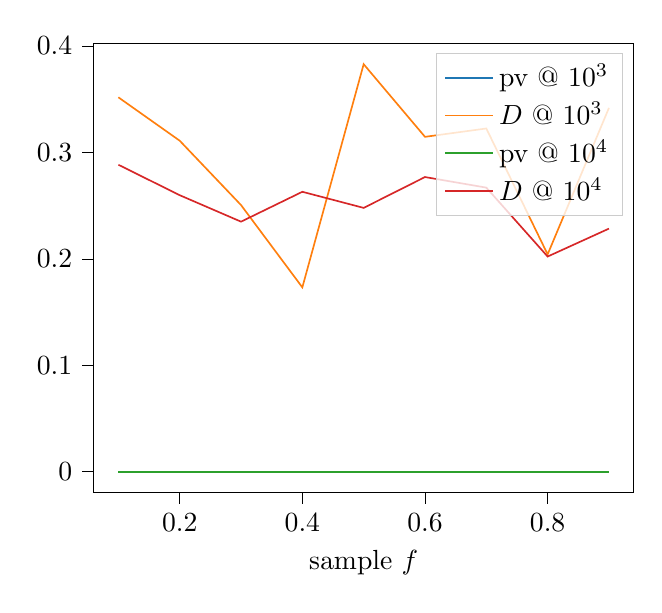
\begin{tikzpicture}

\definecolor{color0}{rgb}{0.12156862745098,0.466666666666667,0.705882352941177}
\definecolor{color1}{rgb}{1,0.498039215686275,0.0549019607843137}
\definecolor{color2}{rgb}{0.172549019607843,0.627450980392157,0.172549019607843}
\definecolor{color3}{rgb}{0.83921568627451,0.152941176470588,0.156862745098039}

\begin{axis}[
legend cell align={left},
legend style={fill opacity=0.8, draw opacity=1, text opacity=1, draw=white!80!black},
tick align=outside,
tick pos=left,
x grid style={white!69.0196078431373!black},
xlabel={sample \(\displaystyle f\)},
xmin=0.06, xmax=0.94,
xtick style={color=black},
y grid style={white!69.0196078431373!black},
ymin=-0.0191365416083822, ymax=0.401867373776027,
ytick style={color=black}
]
\addplot [semithick, color0]
table {%
0.1 8.34942750168255e-52
0.2 3.32481751092495e-47
0.3 5.16830231859641e-28
0.4 1.28543062172452e-10
0.5 6.2648211751132e-65
0.6 2.58092644359044e-27
0.7 9.47422702851892e-37
0.8 2.11154786843285e-11
0.9 1.07913142471793e-39
};
\addlegendentry{pv @ $10^3$}
\addplot [semithick, color1]
table {%
0.1 0.351628735697949
0.2 0.310895032499803
0.3 0.250461812987004
0.4 0.173159578189815
0.5 0.382730832167645
0.6 0.314521446480562
0.7 0.322366469159021
0.8 0.204134801933954
0.9 0.341703279634314
};
\addlegendentry{$D$ @ $10^3$}
\addplot [semithick, color2]
table {%
0.1 0
0.2 0
0.3 0
0.4 0
0.5 0
0.6 0
0.7 0
0.8 0
0.9 0
};
\addlegendentry{pv @ $10^4$}
\addplot [semithick, color3]
table {%
0.1 0.288308985410744
0.2 0.259726112883418
0.3 0.234858619637902
0.4 0.262920136939607
0.5 0.247793276312996
0.6 0.276762380300241
0.7 0.266825918122284
0.8 0.202111801488589
0.9 0.228326612438621
};
\addlegendentry{$D$ @ $10^4$}
\end{axis}

\end{tikzpicture}

	\end{adjustbox}

}\caption{Hash join}
\end{figure}
\begin{figure}
\subfloat[Sample distribution $n=10^{4}$ with $f=0.5$.\label{fig:Stream-join-1}]{    \centering
    \begin{adjustbox}{width=\linewidth,center}
    	% This file was created by tikzplotlib v0.9.8.
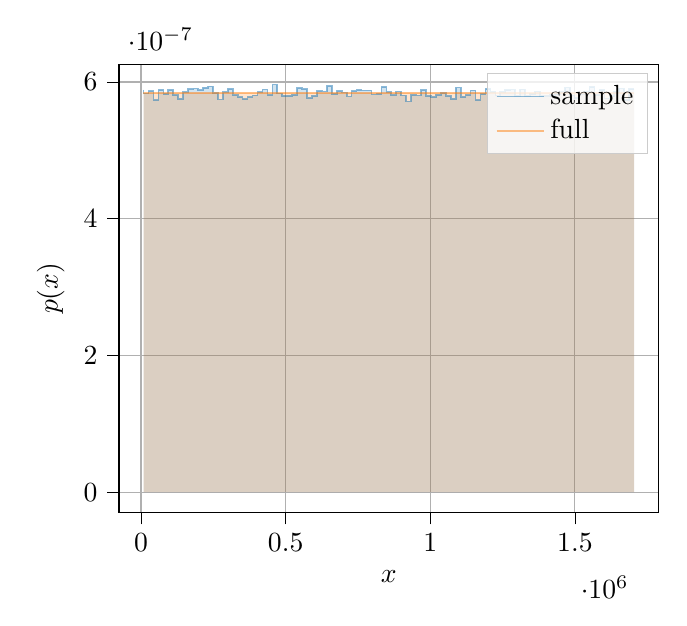
\begin{tikzpicture}

\definecolor{color0}{rgb}{0.12156862745098,0.466666666666667,0.705882352941177}
\definecolor{color1}{rgb}{1,0.498039215686275,0.0549019607843137}

\begin{axis}[
legend cell align={left},
legend style={
  fill opacity=0.8,
  draw opacity=1,
  text opacity=1,
  anchor=north east,
  draw=white!80!black
},
trim axis left,trim axis right,
tick align=outside,
tick pos=left,
%title={n\_rels=2, n\_samps=10000, p=50, alg='streamjoin', stat=0.0009, pval=0.7618},
x grid style={white!69.0196078431373!black},
xmajorgrids,
xmin=-76238.85025, xmax=1789470.82525,
xtick style={color=black},
xlabel={\(\displaystyle x\)},
ylabel={\(\displaystyle p(x)\)},
y grid style={white!69.0196078431373!black},
ymajorgrids,
ymin=-2.98109940785065e-08, ymax=6.26030875648636e-07,
ytick style={color=black},
ylabel near ticks
]
\path [fill=color0, fill opacity=0.2]
(axis cs:8566.135,0)
--(axis cs:8566.135,5.88451988255957e-07)
--(axis cs:8566.135,5.83341532128213e-07)
--(axis cs:25698.405,5.83341532128213e-07)
--(axis cs:25698.405,5.86816642295079e-07)
--(axis cs:42830.675,5.86816642295079e-07)
--(axis cs:42830.675,5.73393177532872e-07)
--(axis cs:59962.945,5.73393177532872e-07)
--(axis cs:59962.945,5.88315709425884e-07)
--(axis cs:77095.215,5.88315709425884e-07)
--(axis cs:77095.215,5.82864556222958e-07)
--(axis cs:94227.485,5.82864556222958e-07)
--(axis cs:94227.485,5.88315709425884e-07)
--(axis cs:111359.755,5.88315709425884e-07)
--(axis cs:111359.755,5.8061595552675e-07)
--(axis cs:128492.025,5.8061595552675e-07)
--(axis cs:128492.025,5.75505499399006e-07)
--(axis cs:145624.295,5.75505499399006e-07)
--(axis cs:145624.295,5.85249435749237e-07)
--(axis cs:162756.565,5.85249435749237e-07)
--(axis cs:162756.565,5.89269661236397e-07)
--(axis cs:179888.835,5.89269661236397e-07)
--(axis cs:179888.835,5.90428031292019e-07)
--(axis cs:197021.105,5.90428031292019e-07)
--(axis cs:197021.105,5.88315709425884e-07)
--(axis cs:214153.375,5.88315709425884e-07)
--(axis cs:214153.375,5.91586401347641e-07)
--(axis cs:231285.645,5.91586401347641e-07)
--(axis cs:231285.645,5.93630583798737e-07)
--(axis cs:248417.915,5.93630583798737e-07)
--(axis cs:248417.915,5.83545950373324e-07)
--(axis cs:265550.185,5.83545950373324e-07)
--(axis cs:265550.185,5.7421085051331e-07)
--(axis cs:282682.455,5.7421085051331e-07)
--(axis cs:282682.455,5.84976878089093e-07)
--(axis cs:299814.725,5.84976878089093e-07)
--(axis cs:299814.725,5.89882915971725e-07)
--(axis cs:316946.995,5.89882915971725e-07)
--(axis cs:316946.995,5.80888513186896e-07)
--(axis cs:334079.265,5.80888513186896e-07)
--(axis cs:334079.265,5.77754100095215e-07)
--(axis cs:351211.535,5.77754100095215e-07)
--(axis cs:351211.535,5.74960384078713e-07)
--(axis cs:368343.805,5.74960384078713e-07)
--(axis cs:368343.805,5.7761782126514e-07)
--(axis cs:385476.075,5.7761782126514e-07)
--(axis cs:385476.075,5.80479676696678e-07)
--(axis cs:402608.345,5.80479676696678e-07)
--(axis cs:402608.345,5.85045017504127e-07)
--(axis cs:419740.615,5.85045017504127e-07)
--(axis cs:419740.615,5.88997103576249e-07)
--(axis cs:436872.885,5.88997103576249e-07)
--(axis cs:436872.885,5.81229210262079e-07)
--(axis cs:454005.155,5.81229210262079e-07)
--(axis cs:454005.155,5.9621988157013e-07)
--(axis cs:471137.425,5.9621988157013e-07)
--(axis cs:471137.425,5.83341532128213e-07)
--(axis cs:488269.695,5.83341532128213e-07)
--(axis cs:488269.695,5.79662003716237e-07)
--(axis cs:505401.965,5.79662003716237e-07)
--(axis cs:505401.965,5.79934561376386e-07)
--(axis cs:522534.235,5.79934561376386e-07)
--(axis cs:522534.235,5.81161070847042e-07)
--(axis cs:539666.505,5.81161070847042e-07)
--(axis cs:539666.505,5.9117756485742e-07)
--(axis cs:556798.775,5.9117756485742e-07)
--(axis cs:556798.775,5.89542218896542e-07)
--(axis cs:573931.045,5.89542218896542e-07)
--(axis cs:573931.045,5.76936427114774e-07)
--(axis cs:591063.315,5.76936427114774e-07)
--(axis cs:591063.315,5.79593864301204e-07)
--(axis cs:608195.585,5.79593864301204e-07)
--(axis cs:608195.585,5.86680363465006e-07)
--(axis cs:625327.855,5.86680363465006e-07)
--(axis cs:625327.855,5.85930829899603e-07)
--(axis cs:642460.125,5.85930829899603e-07)
--(axis cs:642460.125,5.94448256779176e-07)
--(axis cs:659592.395,5.94448256779176e-07)
--(axis cs:659592.395,5.8279641680792e-07)
--(axis cs:676724.665,5.8279641680792e-07)
--(axis cs:676724.665,5.86884781710115e-07)
--(axis cs:693856.935,5.86884781710115e-07)
--(axis cs:693856.935,5.84568041598875e-07)
--(axis cs:710989.205,5.84568041598875e-07)
--(axis cs:710989.205,5.78639912490688e-07)
--(axis cs:728121.475,5.78639912490688e-07)
--(axis cs:728121.475,5.86816642295079e-07)
--(axis cs:745253.745,5.86816642295079e-07)
--(axis cs:745253.745,5.8858826708603e-07)
--(axis cs:762386.015,5.8858826708603e-07)
--(axis cs:762386.015,5.87634315275518e-07)
--(axis cs:779518.285,5.87634315275518e-07)
--(axis cs:779518.285,5.87634315275518e-07)
--(axis cs:796650.555,5.87634315275518e-07)
--(axis cs:796650.555,5.81501767922229e-07)
--(axis cs:813782.825,5.81501767922229e-07)
--(axis cs:813782.825,5.82251301487627e-07)
--(axis cs:830915.095,5.82251301487627e-07)
--(axis cs:830915.095,5.93017329063408e-07)
--(axis cs:848047.365,5.93017329063408e-07)
--(axis cs:848047.365,5.85453853994347e-07)
--(axis cs:865179.635,5.85453853994347e-07)
--(axis cs:865179.635,5.80684094941786e-07)
--(axis cs:882311.905,5.80684094941786e-07)
--(axis cs:882311.905,5.8599896931464e-07)
--(axis cs:899444.175,5.8599896931464e-07)
--(axis cs:899444.175,5.80479676696676e-07)
--(axis cs:916576.445,5.80479676696676e-07)
--(axis cs:916576.445,5.71621552741924e-07)
--(axis cs:933708.715,5.71621552741924e-07)
--(axis cs:933708.715,5.81092931432005e-07)
--(axis cs:950840.985,5.81092931432005e-07)
--(axis cs:950840.985,5.80275258451566e-07)
--(axis cs:967973.255,5.80275258451566e-07)
--(axis cs:967973.255,5.88043151765737e-07)
--(axis cs:985105.525,5.88043151765737e-07)
--(axis cs:985105.525,5.79662003716237e-07)
--(axis cs:1002237.795,5.79662003716237e-07)
--(axis cs:1002237.795,5.77685960680176e-07)
--(axis cs:1019370.065,5.77685960680176e-07)
--(axis cs:1019370.065,5.81365489092156e-07)
--(axis cs:1036502.335,5.81365489092156e-07)
--(axis cs:1036502.335,5.83545950373323e-07)
--(axis cs:1053634.605,5.83545950373323e-07)
--(axis cs:1053634.605,5.79730143131274e-07)
--(axis cs:1070766.875,5.79730143131274e-07)
--(axis cs:1070766.875,5.75573638814042e-07)
--(axis cs:1087899.145,5.75573638814042e-07)
--(axis cs:1087899.145,5.91858959007786e-07)
--(axis cs:1105031.415,5.91858959007786e-07)
--(axis cs:1105031.415,5.78367354830542e-07)
--(axis cs:1122163.685,5.78367354830542e-07)
--(axis cs:1122163.685,5.80956652601932e-07)
--(axis cs:1139295.955,5.80956652601932e-07)
--(axis cs:1139295.955,5.87702454690554e-07)
--(axis cs:1156428.225,5.87702454690554e-07)
--(axis cs:1156428.225,5.73733874608054e-07)
--(axis cs:1173560.495,5.73733874608054e-07)
--(axis cs:1173560.495,5.82387580317701e-07)
--(axis cs:1190692.765,5.82387580317701e-07)
--(axis cs:1190692.765,5.8995105538677e-07)
--(axis cs:1207825.035,5.8995105538677e-07)
--(axis cs:1207825.035,5.85045017504127e-07)
--(axis cs:1224957.305,5.85045017504127e-07)
--(axis cs:1224957.305,5.8020711903653e-07)
--(axis cs:1242089.575,5.8020711903653e-07)
--(axis cs:1242089.575,5.84908738674054e-07)
--(axis cs:1259221.845,5.84908738674054e-07)
--(axis cs:1259221.845,5.88724545916103e-07)
--(axis cs:1276354.115,5.88724545916103e-07)
--(axis cs:1276354.115,5.88997103576249e-07)
--(axis cs:1293486.385,5.88997103576249e-07)
--(axis cs:1293486.385,5.79934561376383e-07)
--(axis cs:1310618.655,5.79934561376383e-07)
--(axis cs:1310618.655,5.89065242991286e-07)
--(axis cs:1327750.925,5.89065242991286e-07)
--(axis cs:1327750.925,5.79525724886164e-07)
--(axis cs:1344883.195,5.79525724886164e-07)
--(axis cs:1344883.195,5.82387580317701e-07)
--(axis cs:1362015.465,5.82387580317701e-07)
--(axis cs:1362015.465,5.86067108729676e-07)
--(axis cs:1379147.735,5.86067108729676e-07)
--(axis cs:1379147.735,5.79730143131274e-07)
--(axis cs:1396280.005,5.79730143131274e-07)
--(axis cs:1396280.005,5.79116888395944e-07)
--(axis cs:1413412.275,5.79116888395944e-07)
--(axis cs:1413412.275,5.80547816111721e-07)
--(axis cs:1430544.545,5.80547816111721e-07)
--(axis cs:1430544.545,5.82251301487627e-07)
--(axis cs:1447676.815,5.82251301487627e-07)
--(axis cs:1447676.815,5.84908738674054e-07)
--(axis cs:1464809.085,5.84908738674054e-07)
--(axis cs:1464809.085,5.9179081959275e-07)
--(axis cs:1481941.355,5.9179081959275e-07)
--(axis cs:1481941.355,5.80275258451566e-07)
--(axis cs:1499073.625,5.80275258451566e-07)
--(axis cs:1499073.625,5.76186893549371e-07)
--(axis cs:1516205.895,5.76186893549371e-07)
--(axis cs:1516205.895,5.81978743827481e-07)
--(axis cs:1533338.165,5.81978743827481e-07)
--(axis cs:1533338.165,5.85317575164274e-07)
--(axis cs:1550470.435,5.85317575164274e-07)
--(axis cs:1550470.435,5.92812910818298e-07)
--(axis cs:1567602.705,5.92812910818298e-07)
--(axis cs:1567602.705,5.80547816111713e-07)
--(axis cs:1584734.975,5.80547816111713e-07)
--(axis cs:1584734.975,5.87838733520627e-07)
--(axis cs:1601867.245,5.87838733520627e-07)
--(axis cs:1601867.245,5.75914335889225e-07)
--(axis cs:1618999.515,5.75914335889225e-07)
--(axis cs:1618999.515,5.79525724886172e-07)
--(axis cs:1636131.785,5.79525724886172e-07)
--(axis cs:1636131.785,5.85317575164274e-07)
--(axis cs:1653264.055,5.85317575164274e-07)
--(axis cs:1653264.055,5.90359891876981e-07)
--(axis cs:1670396.325,5.90359891876981e-07)
--(axis cs:1670396.325,5.73870153438127e-07)
--(axis cs:1687528.595,5.73870153438127e-07)
--(axis cs:1687528.595,5.89405940066469e-07)
--(axis cs:1704660.865,5.89405940066469e-07)
--(axis cs:1704660.865,0)
--(axis cs:1704660.865,0)
--(axis cs:1687528.595,0)
--(axis cs:1687528.595,0)
--(axis cs:1670396.325,0)
--(axis cs:1670396.325,0)
--(axis cs:1653264.055,0)
--(axis cs:1653264.055,0)
--(axis cs:1636131.785,0)
--(axis cs:1636131.785,0)
--(axis cs:1618999.515,0)
--(axis cs:1618999.515,0)
--(axis cs:1601867.245,0)
--(axis cs:1601867.245,0)
--(axis cs:1584734.975,0)
--(axis cs:1584734.975,0)
--(axis cs:1567602.705,0)
--(axis cs:1567602.705,0)
--(axis cs:1550470.435,0)
--(axis cs:1550470.435,0)
--(axis cs:1533338.165,0)
--(axis cs:1533338.165,0)
--(axis cs:1516205.895,0)
--(axis cs:1516205.895,0)
--(axis cs:1499073.625,0)
--(axis cs:1499073.625,0)
--(axis cs:1481941.355,0)
--(axis cs:1481941.355,0)
--(axis cs:1464809.085,0)
--(axis cs:1464809.085,0)
--(axis cs:1447676.815,0)
--(axis cs:1447676.815,0)
--(axis cs:1430544.545,0)
--(axis cs:1430544.545,0)
--(axis cs:1413412.275,0)
--(axis cs:1413412.275,0)
--(axis cs:1396280.005,0)
--(axis cs:1396280.005,0)
--(axis cs:1379147.735,0)
--(axis cs:1379147.735,0)
--(axis cs:1362015.465,0)
--(axis cs:1362015.465,0)
--(axis cs:1344883.195,0)
--(axis cs:1344883.195,0)
--(axis cs:1327750.925,0)
--(axis cs:1327750.925,0)
--(axis cs:1310618.655,0)
--(axis cs:1310618.655,0)
--(axis cs:1293486.385,0)
--(axis cs:1293486.385,0)
--(axis cs:1276354.115,0)
--(axis cs:1276354.115,0)
--(axis cs:1259221.845,0)
--(axis cs:1259221.845,0)
--(axis cs:1242089.575,0)
--(axis cs:1242089.575,0)
--(axis cs:1224957.305,0)
--(axis cs:1224957.305,0)
--(axis cs:1207825.035,0)
--(axis cs:1207825.035,0)
--(axis cs:1190692.765,0)
--(axis cs:1190692.765,0)
--(axis cs:1173560.495,0)
--(axis cs:1173560.495,0)
--(axis cs:1156428.225,0)
--(axis cs:1156428.225,0)
--(axis cs:1139295.955,0)
--(axis cs:1139295.955,0)
--(axis cs:1122163.685,0)
--(axis cs:1122163.685,0)
--(axis cs:1105031.415,0)
--(axis cs:1105031.415,0)
--(axis cs:1087899.145,0)
--(axis cs:1087899.145,0)
--(axis cs:1070766.875,0)
--(axis cs:1070766.875,0)
--(axis cs:1053634.605,0)
--(axis cs:1053634.605,0)
--(axis cs:1036502.335,0)
--(axis cs:1036502.335,0)
--(axis cs:1019370.065,0)
--(axis cs:1019370.065,0)
--(axis cs:1002237.795,0)
--(axis cs:1002237.795,0)
--(axis cs:985105.525,0)
--(axis cs:985105.525,0)
--(axis cs:967973.255,0)
--(axis cs:967973.255,0)
--(axis cs:950840.985,0)
--(axis cs:950840.985,0)
--(axis cs:933708.715,0)
--(axis cs:933708.715,0)
--(axis cs:916576.445,0)
--(axis cs:916576.445,0)
--(axis cs:899444.175,0)
--(axis cs:899444.175,0)
--(axis cs:882311.905,0)
--(axis cs:882311.905,0)
--(axis cs:865179.635,0)
--(axis cs:865179.635,0)
--(axis cs:848047.365,0)
--(axis cs:848047.365,0)
--(axis cs:830915.095,0)
--(axis cs:830915.095,0)
--(axis cs:813782.825,0)
--(axis cs:813782.825,0)
--(axis cs:796650.555,0)
--(axis cs:796650.555,0)
--(axis cs:779518.285,0)
--(axis cs:779518.285,0)
--(axis cs:762386.015,0)
--(axis cs:762386.015,0)
--(axis cs:745253.745,0)
--(axis cs:745253.745,0)
--(axis cs:728121.475,0)
--(axis cs:728121.475,0)
--(axis cs:710989.205,0)
--(axis cs:710989.205,0)
--(axis cs:693856.935,0)
--(axis cs:693856.935,0)
--(axis cs:676724.665,0)
--(axis cs:676724.665,0)
--(axis cs:659592.395,0)
--(axis cs:659592.395,0)
--(axis cs:642460.125,0)
--(axis cs:642460.125,0)
--(axis cs:625327.855,0)
--(axis cs:625327.855,0)
--(axis cs:608195.585,0)
--(axis cs:608195.585,0)
--(axis cs:591063.315,0)
--(axis cs:591063.315,0)
--(axis cs:573931.045,0)
--(axis cs:573931.045,0)
--(axis cs:556798.775,0)
--(axis cs:556798.775,0)
--(axis cs:539666.505,0)
--(axis cs:539666.505,0)
--(axis cs:522534.235,0)
--(axis cs:522534.235,0)
--(axis cs:505401.965,0)
--(axis cs:505401.965,0)
--(axis cs:488269.695,0)
--(axis cs:488269.695,0)
--(axis cs:471137.425,0)
--(axis cs:471137.425,0)
--(axis cs:454005.155,0)
--(axis cs:454005.155,0)
--(axis cs:436872.885,0)
--(axis cs:436872.885,0)
--(axis cs:419740.615,0)
--(axis cs:419740.615,0)
--(axis cs:402608.345,0)
--(axis cs:402608.345,0)
--(axis cs:385476.075,0)
--(axis cs:385476.075,0)
--(axis cs:368343.805,0)
--(axis cs:368343.805,0)
--(axis cs:351211.535,0)
--(axis cs:351211.535,0)
--(axis cs:334079.265,0)
--(axis cs:334079.265,0)
--(axis cs:316946.995,0)
--(axis cs:316946.995,0)
--(axis cs:299814.725,0)
--(axis cs:299814.725,0)
--(axis cs:282682.455,0)
--(axis cs:282682.455,0)
--(axis cs:265550.185,0)
--(axis cs:265550.185,0)
--(axis cs:248417.915,0)
--(axis cs:248417.915,0)
--(axis cs:231285.645,0)
--(axis cs:231285.645,0)
--(axis cs:214153.375,0)
--(axis cs:214153.375,0)
--(axis cs:197021.105,0)
--(axis cs:197021.105,0)
--(axis cs:179888.835,0)
--(axis cs:179888.835,0)
--(axis cs:162756.565,0)
--(axis cs:162756.565,0)
--(axis cs:145624.295,0)
--(axis cs:145624.295,0)
--(axis cs:128492.025,0)
--(axis cs:128492.025,0)
--(axis cs:111359.755,0)
--(axis cs:111359.755,0)
--(axis cs:94227.485,0)
--(axis cs:94227.485,0)
--(axis cs:77095.215,0)
--(axis cs:77095.215,0)
--(axis cs:59962.945,0)
--(axis cs:59962.945,0)
--(axis cs:42830.675,0)
--(axis cs:42830.675,0)
--(axis cs:25698.405,0)
--(axis cs:25698.405,0)
--(axis cs:8566.135,0)
--(axis cs:8566.135,0)
--cycle;

\path [fill=color1, fill opacity=0.2]
(axis cs:8566.16,0)
--(axis cs:8566.16,5.8371493606733e-07)
--(axis cs:8566.16,5.83680866439357e-07)
--(axis cs:25698.48,5.83680866439357e-07)
--(axis cs:25698.48,5.83680866439357e-07)
--(axis cs:42830.8,5.83680866439357e-07)
--(axis cs:42830.8,5.8371493606733e-07)
--(axis cs:59963.12,5.8371493606733e-07)
--(axis cs:59963.12,5.83680866439357e-07)
--(axis cs:77095.44,5.83680866439357e-07)
--(axis cs:77095.44,5.83680866439357e-07)
--(axis cs:94227.76,5.83680866439357e-07)
--(axis cs:94227.76,5.83714936067331e-07)
--(axis cs:111360.08,5.83714936067331e-07)
--(axis cs:111360.08,5.83680866439357e-07)
--(axis cs:128492.4,5.83680866439357e-07)
--(axis cs:128492.4,5.83680866439357e-07)
--(axis cs:145624.72,5.83680866439357e-07)
--(axis cs:145624.72,5.8371493606733e-07)
--(axis cs:162757.04,5.8371493606733e-07)
--(axis cs:162757.04,5.83680866439358e-07)
--(axis cs:179889.36,5.83680866439358e-07)
--(axis cs:179889.36,5.83680866439357e-07)
--(axis cs:197021.68,5.83680866439357e-07)
--(axis cs:197021.68,5.8371493606733e-07)
--(axis cs:214154,5.8371493606733e-07)
--(axis cs:214154,5.83680866439358e-07)
--(axis cs:231286.32,5.83680866439358e-07)
--(axis cs:231286.32,5.83680866439357e-07)
--(axis cs:248418.64,5.83680866439357e-07)
--(axis cs:248418.64,5.8371493606733e-07)
--(axis cs:265550.96,5.8371493606733e-07)
--(axis cs:265550.96,5.83680866439357e-07)
--(axis cs:282683.28,5.83680866439357e-07)
--(axis cs:282683.28,5.83680866439357e-07)
--(axis cs:299815.6,5.83680866439357e-07)
--(axis cs:299815.6,5.8371493606733e-07)
--(axis cs:316947.92,5.8371493606733e-07)
--(axis cs:316947.92,5.83680866439357e-07)
--(axis cs:334080.24,5.83680866439357e-07)
--(axis cs:334080.24,5.83680866439359e-07)
--(axis cs:351212.56,5.83680866439359e-07)
--(axis cs:351212.56,5.8371493606733e-07)
--(axis cs:368344.88,5.8371493606733e-07)
--(axis cs:368344.88,5.83680866439357e-07)
--(axis cs:385477.2,5.83680866439357e-07)
--(axis cs:385477.2,5.83680866439357e-07)
--(axis cs:402609.52,5.83680866439357e-07)
--(axis cs:402609.52,5.83680866439357e-07)
--(axis cs:419741.84,5.83680866439357e-07)
--(axis cs:419741.84,5.8371493606733e-07)
--(axis cs:436874.16,5.8371493606733e-07)
--(axis cs:436874.16,5.83680866439357e-07)
--(axis cs:454006.48,5.83680866439357e-07)
--(axis cs:454006.48,5.83680866439359e-07)
--(axis cs:471138.8,5.83680866439359e-07)
--(axis cs:471138.8,5.8371493606733e-07)
--(axis cs:488271.12,5.8371493606733e-07)
--(axis cs:488271.12,5.83680866439357e-07)
--(axis cs:505403.44,5.83680866439357e-07)
--(axis cs:505403.44,5.83680866439355e-07)
--(axis cs:522535.76,5.83680866439355e-07)
--(axis cs:522535.76,5.83714936067332e-07)
--(axis cs:539668.08,5.83714936067332e-07)
--(axis cs:539668.08,5.83680866439359e-07)
--(axis cs:556800.4,5.83680866439359e-07)
--(axis cs:556800.4,5.83680866439355e-07)
--(axis cs:573932.72,5.83680866439355e-07)
--(axis cs:573932.72,5.83714936067332e-07)
--(axis cs:591065.04,5.83714936067332e-07)
--(axis cs:591065.04,5.83680866439355e-07)
--(axis cs:608197.36,5.83680866439355e-07)
--(axis cs:608197.36,5.83680866439359e-07)
--(axis cs:625329.68,5.83680866439359e-07)
--(axis cs:625329.68,5.83714936067328e-07)
--(axis cs:642462,5.83714936067328e-07)
--(axis cs:642462,5.83680866439359e-07)
--(axis cs:659594.32,5.83680866439359e-07)
--(axis cs:659594.32,5.83680866439355e-07)
--(axis cs:676726.64,5.83680866439355e-07)
--(axis cs:676726.64,5.83714936067332e-07)
--(axis cs:693858.96,5.83714936067332e-07)
--(axis cs:693858.96,5.83680866439359e-07)
--(axis cs:710991.28,5.83680866439359e-07)
--(axis cs:710991.28,5.83680866439355e-07)
--(axis cs:728123.6,5.83680866439355e-07)
--(axis cs:728123.6,5.83714936067332e-07)
--(axis cs:745255.92,5.83714936067332e-07)
--(axis cs:745255.92,5.83680866439355e-07)
--(axis cs:762388.24,5.83680866439355e-07)
--(axis cs:762388.24,5.83680866439359e-07)
--(axis cs:779520.56,5.83680866439359e-07)
--(axis cs:779520.56,5.83714936067328e-07)
--(axis cs:796652.88,5.83714936067328e-07)
--(axis cs:796652.88,5.83680866439359e-07)
--(axis cs:813785.2,5.83680866439359e-07)
--(axis cs:813785.2,5.83680866439359e-07)
--(axis cs:830917.52,5.83680866439359e-07)
--(axis cs:830917.52,5.83680866439355e-07)
--(axis cs:848049.84,5.83680866439355e-07)
--(axis cs:848049.84,5.83714936067332e-07)
--(axis cs:865182.16,5.83714936067332e-07)
--(axis cs:865182.16,5.83680866439355e-07)
--(axis cs:882314.48,5.83680866439355e-07)
--(axis cs:882314.48,5.83680866439359e-07)
--(axis cs:899446.8,5.83680866439359e-07)
--(axis cs:899446.8,5.83714936067328e-07)
--(axis cs:916579.12,5.83714936067328e-07)
--(axis cs:916579.12,5.83680866439359e-07)
--(axis cs:933711.44,5.83680866439359e-07)
--(axis cs:933711.44,5.83680866439359e-07)
--(axis cs:950843.76,5.83680866439359e-07)
--(axis cs:950843.76,5.83714936067328e-07)
--(axis cs:967976.08,5.83714936067328e-07)
--(axis cs:967976.08,5.83680866439359e-07)
--(axis cs:985108.4,5.83680866439359e-07)
--(axis cs:985108.4,5.83680866439355e-07)
--(axis cs:1002240.72,5.83680866439355e-07)
--(axis cs:1002240.72,5.83714936067332e-07)
--(axis cs:1019373.04,5.83714936067332e-07)
--(axis cs:1019373.04,5.83680866439355e-07)
--(axis cs:1036505.36,5.83680866439355e-07)
--(axis cs:1036505.36,5.83680866439355e-07)
--(axis cs:1053637.68,5.83680866439355e-07)
--(axis cs:1053637.68,5.83714936067336e-07)
--(axis cs:1070770,5.83714936067336e-07)
--(axis cs:1070770,5.83680866439355e-07)
--(axis cs:1087902.32,5.83680866439355e-07)
--(axis cs:1087902.32,5.83680866439355e-07)
--(axis cs:1105034.64,5.83680866439355e-07)
--(axis cs:1105034.64,5.83714936067336e-07)
--(axis cs:1122166.96,5.83714936067336e-07)
--(axis cs:1122166.96,5.83680866439355e-07)
--(axis cs:1139299.28,5.83680866439355e-07)
--(axis cs:1139299.28,5.83680866439355e-07)
--(axis cs:1156431.6,5.83680866439355e-07)
--(axis cs:1156431.6,5.83714936067328e-07)
--(axis cs:1173563.92,5.83714936067328e-07)
--(axis cs:1173563.92,5.83680866439363e-07)
--(axis cs:1190696.24,5.83680866439363e-07)
--(axis cs:1190696.24,5.83680866439355e-07)
--(axis cs:1207828.56,5.83680866439355e-07)
--(axis cs:1207828.56,5.83714936067328e-07)
--(axis cs:1224960.88,5.83714936067328e-07)
--(axis cs:1224960.88,5.83680866439363e-07)
--(axis cs:1242093.2,5.83680866439363e-07)
--(axis cs:1242093.2,5.83680866439355e-07)
--(axis cs:1259225.52,5.83680866439355e-07)
--(axis cs:1259225.52,5.83680866439355e-07)
--(axis cs:1276357.84,5.83680866439355e-07)
--(axis cs:1276357.84,5.83714936067328e-07)
--(axis cs:1293490.16,5.83714936067328e-07)
--(axis cs:1293490.16,5.83680866439363e-07)
--(axis cs:1310622.48,5.83680866439363e-07)
--(axis cs:1310622.48,5.83680866439355e-07)
--(axis cs:1327754.8,5.83680866439355e-07)
--(axis cs:1327754.8,5.83714936067328e-07)
--(axis cs:1344887.12,5.83714936067328e-07)
--(axis cs:1344887.12,5.83680866439355e-07)
--(axis cs:1362019.44,5.83680866439355e-07)
--(axis cs:1362019.44,5.83680866439363e-07)
--(axis cs:1379151.76,5.83680866439363e-07)
--(axis cs:1379151.76,5.83714936067328e-07)
--(axis cs:1396284.08,5.83714936067328e-07)
--(axis cs:1396284.08,5.83680866439355e-07)
--(axis cs:1413416.4,5.83680866439355e-07)
--(axis cs:1413416.4,5.83680866439363e-07)
--(axis cs:1430548.72,5.83680866439363e-07)
--(axis cs:1430548.72,5.83714936067328e-07)
--(axis cs:1447681.04,5.83714936067328e-07)
--(axis cs:1447681.04,5.83680866439355e-07)
--(axis cs:1464813.36,5.83680866439355e-07)
--(axis cs:1464813.36,5.83680866439355e-07)
--(axis cs:1481945.68,5.83680866439355e-07)
--(axis cs:1481945.68,5.83714936067336e-07)
--(axis cs:1499078,5.83714936067336e-07)
--(axis cs:1499078,5.83680866439355e-07)
--(axis cs:1516210.32,5.83680866439355e-07)
--(axis cs:1516210.32,5.83680866439355e-07)
--(axis cs:1533342.64,5.83680866439355e-07)
--(axis cs:1533342.64,5.83714936067336e-07)
--(axis cs:1550474.96,5.83714936067336e-07)
--(axis cs:1550474.96,5.83680866439355e-07)
--(axis cs:1567607.28,5.83680866439355e-07)
--(axis cs:1567607.28,5.83680866439355e-07)
--(axis cs:1584739.6,5.83680866439355e-07)
--(axis cs:1584739.6,5.83714936067328e-07)
--(axis cs:1601871.92,5.83714936067328e-07)
--(axis cs:1601871.92,5.83680866439363e-07)
--(axis cs:1619004.24,5.83680866439363e-07)
--(axis cs:1619004.24,5.83680866439355e-07)
--(axis cs:1636136.56,5.83680866439355e-07)
--(axis cs:1636136.56,5.83714936067328e-07)
--(axis cs:1653268.88,5.83714936067328e-07)
--(axis cs:1653268.88,5.83680866439363e-07)
--(axis cs:1670401.2,5.83680866439363e-07)
--(axis cs:1670401.2,5.83680866439355e-07)
--(axis cs:1687533.52,5.83680866439355e-07)
--(axis cs:1687533.52,5.83714936067328e-07)
--(axis cs:1704665.84,5.83714936067328e-07)
--(axis cs:1704665.84,0)
--(axis cs:1704665.84,0)
--(axis cs:1687533.52,0)
--(axis cs:1687533.52,0)
--(axis cs:1670401.2,0)
--(axis cs:1670401.2,0)
--(axis cs:1653268.88,0)
--(axis cs:1653268.88,0)
--(axis cs:1636136.56,0)
--(axis cs:1636136.56,0)
--(axis cs:1619004.24,0)
--(axis cs:1619004.24,0)
--(axis cs:1601871.92,0)
--(axis cs:1601871.92,0)
--(axis cs:1584739.6,0)
--(axis cs:1584739.6,0)
--(axis cs:1567607.28,0)
--(axis cs:1567607.28,0)
--(axis cs:1550474.96,0)
--(axis cs:1550474.96,0)
--(axis cs:1533342.64,0)
--(axis cs:1533342.64,0)
--(axis cs:1516210.32,0)
--(axis cs:1516210.32,0)
--(axis cs:1499078,0)
--(axis cs:1499078,0)
--(axis cs:1481945.68,0)
--(axis cs:1481945.68,0)
--(axis cs:1464813.36,0)
--(axis cs:1464813.36,0)
--(axis cs:1447681.04,0)
--(axis cs:1447681.04,0)
--(axis cs:1430548.72,0)
--(axis cs:1430548.72,0)
--(axis cs:1413416.4,0)
--(axis cs:1413416.4,0)
--(axis cs:1396284.08,0)
--(axis cs:1396284.08,0)
--(axis cs:1379151.76,0)
--(axis cs:1379151.76,0)
--(axis cs:1362019.44,0)
--(axis cs:1362019.44,0)
--(axis cs:1344887.12,0)
--(axis cs:1344887.12,0)
--(axis cs:1327754.8,0)
--(axis cs:1327754.8,0)
--(axis cs:1310622.48,0)
--(axis cs:1310622.48,0)
--(axis cs:1293490.16,0)
--(axis cs:1293490.16,0)
--(axis cs:1276357.84,0)
--(axis cs:1276357.84,0)
--(axis cs:1259225.52,0)
--(axis cs:1259225.52,0)
--(axis cs:1242093.2,0)
--(axis cs:1242093.2,0)
--(axis cs:1224960.88,0)
--(axis cs:1224960.88,0)
--(axis cs:1207828.56,0)
--(axis cs:1207828.56,0)
--(axis cs:1190696.24,0)
--(axis cs:1190696.24,0)
--(axis cs:1173563.92,0)
--(axis cs:1173563.92,0)
--(axis cs:1156431.6,0)
--(axis cs:1156431.6,0)
--(axis cs:1139299.28,0)
--(axis cs:1139299.28,0)
--(axis cs:1122166.96,0)
--(axis cs:1122166.96,0)
--(axis cs:1105034.64,0)
--(axis cs:1105034.64,0)
--(axis cs:1087902.32,0)
--(axis cs:1087902.32,0)
--(axis cs:1070770,0)
--(axis cs:1070770,0)
--(axis cs:1053637.68,0)
--(axis cs:1053637.68,0)
--(axis cs:1036505.36,0)
--(axis cs:1036505.36,0)
--(axis cs:1019373.04,0)
--(axis cs:1019373.04,0)
--(axis cs:1002240.72,0)
--(axis cs:1002240.72,0)
--(axis cs:985108.4,0)
--(axis cs:985108.4,0)
--(axis cs:967976.08,0)
--(axis cs:967976.08,0)
--(axis cs:950843.76,0)
--(axis cs:950843.76,0)
--(axis cs:933711.44,0)
--(axis cs:933711.44,0)
--(axis cs:916579.12,0)
--(axis cs:916579.12,0)
--(axis cs:899446.8,0)
--(axis cs:899446.8,0)
--(axis cs:882314.48,0)
--(axis cs:882314.48,0)
--(axis cs:865182.16,0)
--(axis cs:865182.16,0)
--(axis cs:848049.84,0)
--(axis cs:848049.84,0)
--(axis cs:830917.52,0)
--(axis cs:830917.52,0)
--(axis cs:813785.2,0)
--(axis cs:813785.2,0)
--(axis cs:796652.88,0)
--(axis cs:796652.88,0)
--(axis cs:779520.56,0)
--(axis cs:779520.56,0)
--(axis cs:762388.24,0)
--(axis cs:762388.24,0)
--(axis cs:745255.92,0)
--(axis cs:745255.92,0)
--(axis cs:728123.6,0)
--(axis cs:728123.6,0)
--(axis cs:710991.28,0)
--(axis cs:710991.28,0)
--(axis cs:693858.96,0)
--(axis cs:693858.96,0)
--(axis cs:676726.64,0)
--(axis cs:676726.64,0)
--(axis cs:659594.32,0)
--(axis cs:659594.32,0)
--(axis cs:642462,0)
--(axis cs:642462,0)
--(axis cs:625329.68,0)
--(axis cs:625329.68,0)
--(axis cs:608197.36,0)
--(axis cs:608197.36,0)
--(axis cs:591065.04,0)
--(axis cs:591065.04,0)
--(axis cs:573932.72,0)
--(axis cs:573932.72,0)
--(axis cs:556800.4,0)
--(axis cs:556800.4,0)
--(axis cs:539668.08,0)
--(axis cs:539668.08,0)
--(axis cs:522535.76,0)
--(axis cs:522535.76,0)
--(axis cs:505403.44,0)
--(axis cs:505403.44,0)
--(axis cs:488271.12,0)
--(axis cs:488271.12,0)
--(axis cs:471138.8,0)
--(axis cs:471138.8,0)
--(axis cs:454006.48,0)
--(axis cs:454006.48,0)
--(axis cs:436874.16,0)
--(axis cs:436874.16,0)
--(axis cs:419741.84,0)
--(axis cs:419741.84,0)
--(axis cs:402609.52,0)
--(axis cs:402609.52,0)
--(axis cs:385477.2,0)
--(axis cs:385477.2,0)
--(axis cs:368344.88,0)
--(axis cs:368344.88,0)
--(axis cs:351212.56,0)
--(axis cs:351212.56,0)
--(axis cs:334080.24,0)
--(axis cs:334080.24,0)
--(axis cs:316947.92,0)
--(axis cs:316947.92,0)
--(axis cs:299815.6,0)
--(axis cs:299815.6,0)
--(axis cs:282683.28,0)
--(axis cs:282683.28,0)
--(axis cs:265550.96,0)
--(axis cs:265550.96,0)
--(axis cs:248418.64,0)
--(axis cs:248418.64,0)
--(axis cs:231286.32,0)
--(axis cs:231286.32,0)
--(axis cs:214154,0)
--(axis cs:214154,0)
--(axis cs:197021.68,0)
--(axis cs:197021.68,0)
--(axis cs:179889.36,0)
--(axis cs:179889.36,0)
--(axis cs:162757.04,0)
--(axis cs:162757.04,0)
--(axis cs:145624.72,0)
--(axis cs:145624.72,0)
--(axis cs:128492.4,0)
--(axis cs:128492.4,0)
--(axis cs:111360.08,0)
--(axis cs:111360.08,0)
--(axis cs:94227.76,0)
--(axis cs:94227.76,0)
--(axis cs:77095.44,0)
--(axis cs:77095.44,0)
--(axis cs:59963.12,0)
--(axis cs:59963.12,0)
--(axis cs:42830.8,0)
--(axis cs:42830.8,0)
--(axis cs:25698.48,0)
--(axis cs:25698.48,0)
--(axis cs:8566.16,0)
--(axis cs:8566.16,0)
--cycle;

\addplot [semithick, color0, const plot mark right, opacity=0.5]
table {%
8566.135 5.88451988255957e-07
25698.405 5.83341532128213e-07
42830.675 5.86816642295079e-07
59962.945 5.73393177532872e-07
77095.215 5.88315709425884e-07
94227.485 5.82864556222958e-07
111359.755 5.88315709425884e-07
128492.025 5.8061595552675e-07
145624.295 5.75505499399006e-07
162756.565 5.85249435749237e-07
179888.835 5.89269661236397e-07
197021.105 5.90428031292019e-07
214153.375 5.88315709425884e-07
231285.645 5.91586401347641e-07
248417.915 5.93630583798737e-07
265550.185 5.83545950373324e-07
282682.455 5.7421085051331e-07
299814.725 5.84976878089093e-07
316946.995 5.89882915971725e-07
334079.265 5.80888513186896e-07
351211.535 5.77754100095215e-07
368343.805 5.74960384078713e-07
385476.075 5.7761782126514e-07
402608.345 5.80479676696678e-07
419740.615 5.85045017504127e-07
436872.885 5.88997103576249e-07
454005.155 5.81229210262079e-07
471137.425 5.9621988157013e-07
488269.695 5.83341532128213e-07
505401.965 5.79662003716237e-07
522534.235 5.79934561376386e-07
539666.505 5.81161070847042e-07
556798.775 5.9117756485742e-07
573931.045 5.89542218896542e-07
591063.315 5.76936427114774e-07
608195.585 5.79593864301204e-07
625327.855 5.86680363465006e-07
642460.125 5.85930829899603e-07
659592.395 5.94448256779176e-07
676724.665 5.8279641680792e-07
693856.935 5.86884781710115e-07
710989.205 5.84568041598875e-07
728121.475 5.78639912490688e-07
745253.745 5.86816642295079e-07
762386.015 5.8858826708603e-07
779518.285 5.87634315275518e-07
796650.555 5.87634315275518e-07
813782.825 5.81501767922229e-07
830915.095 5.82251301487627e-07
848047.365 5.93017329063408e-07
865179.635 5.85453853994347e-07
882311.905 5.80684094941786e-07
899444.175 5.8599896931464e-07
916576.445 5.80479676696676e-07
933708.715 5.71621552741924e-07
950840.985 5.81092931432005e-07
967973.255 5.80275258451566e-07
985105.525 5.88043151765737e-07
1002237.795 5.79662003716237e-07
1019370.065 5.77685960680176e-07
1036502.335 5.81365489092156e-07
1053634.605 5.83545950373323e-07
1070766.875 5.79730143131274e-07
1087899.145 5.75573638814042e-07
1105031.415 5.91858959007786e-07
1122163.685 5.78367354830542e-07
1139295.955 5.80956652601932e-07
1156428.225 5.87702454690554e-07
1173560.495 5.73733874608054e-07
1190692.765 5.82387580317701e-07
1207825.035 5.8995105538677e-07
1224957.305 5.85045017504127e-07
1242089.575 5.8020711903653e-07
1259221.845 5.84908738674054e-07
1276354.115 5.88724545916103e-07
1293486.385 5.88997103576249e-07
1310618.655 5.79934561376383e-07
1327750.925 5.89065242991286e-07
1344883.195 5.79525724886164e-07
1362015.465 5.82387580317701e-07
1379147.735 5.86067108729676e-07
1396280.005 5.79730143131274e-07
1413412.275 5.79116888395944e-07
1430544.545 5.80547816111721e-07
1447676.815 5.82251301487627e-07
1464809.085 5.84908738674054e-07
1481941.355 5.9179081959275e-07
1499073.625 5.80275258451566e-07
1516205.895 5.76186893549371e-07
1533338.165 5.81978743827481e-07
1550470.435 5.85317575164274e-07
1567602.705 5.92812910818298e-07
1584734.975 5.80547816111713e-07
1601867.245 5.87838733520627e-07
1618999.515 5.75914335889225e-07
1636131.785 5.79525724886172e-07
1653264.055 5.85317575164274e-07
1670396.325 5.90359891876981e-07
1687528.595 5.73870153438127e-07
1704660.865 5.89405940066469e-07
};
\addlegendentry{sample}
\addplot [semithick, color1, const plot mark right, opacity=0.5]
table {%
8566.16 5.8371493606733e-07
25698.48 5.83680866439357e-07
42830.8 5.83680866439357e-07
59963.12 5.8371493606733e-07
77095.44 5.83680866439357e-07
94227.76 5.83680866439357e-07
111360.08 5.83714936067331e-07
128492.4 5.83680866439357e-07
145624.72 5.83680866439357e-07
162757.04 5.8371493606733e-07
179889.36 5.83680866439358e-07
197021.68 5.83680866439357e-07
214154 5.8371493606733e-07
231286.32 5.83680866439358e-07
248418.64 5.83680866439357e-07
265550.96 5.8371493606733e-07
282683.28 5.83680866439357e-07
299815.6 5.83680866439357e-07
316947.92 5.8371493606733e-07
334080.24 5.83680866439357e-07
351212.56 5.83680866439359e-07
368344.88 5.8371493606733e-07
385477.2 5.83680866439357e-07
402609.52 5.83680866439357e-07
419741.84 5.83680866439357e-07
436874.16 5.8371493606733e-07
454006.48 5.83680866439357e-07
471138.8 5.83680866439359e-07
488271.12 5.8371493606733e-07
505403.44 5.83680866439357e-07
522535.76 5.83680866439355e-07
539668.08 5.83714936067332e-07
556800.4 5.83680866439359e-07
573932.72 5.83680866439355e-07
591065.04 5.83714936067332e-07
608197.36 5.83680866439355e-07
625329.68 5.83680866439359e-07
642462 5.83714936067328e-07
659594.32 5.83680866439359e-07
676726.64 5.83680866439355e-07
693858.96 5.83714936067332e-07
710991.28 5.83680866439359e-07
728123.6 5.83680866439355e-07
745255.92 5.83714936067332e-07
762388.24 5.83680866439355e-07
779520.56 5.83680866439359e-07
796652.88 5.83714936067328e-07
813785.2 5.83680866439359e-07
830917.52 5.83680866439359e-07
848049.84 5.83680866439355e-07
865182.16 5.83714936067332e-07
882314.48 5.83680866439355e-07
899446.8 5.83680866439359e-07
916579.12 5.83714936067328e-07
933711.44 5.83680866439359e-07
950843.76 5.83680866439359e-07
967976.08 5.83714936067328e-07
985108.4 5.83680866439359e-07
1002240.72 5.83680866439355e-07
1019373.04 5.83714936067332e-07
1036505.36 5.83680866439355e-07
1053637.68 5.83680866439355e-07
1070770 5.83714936067336e-07
1087902.32 5.83680866439355e-07
1105034.64 5.83680866439355e-07
1122166.96 5.83714936067336e-07
1139299.28 5.83680866439355e-07
1156431.6 5.83680866439355e-07
1173563.92 5.83714936067328e-07
1190696.24 5.83680866439363e-07
1207828.56 5.83680866439355e-07
1224960.88 5.83714936067328e-07
1242093.2 5.83680866439363e-07
1259225.52 5.83680866439355e-07
1276357.84 5.83680866439355e-07
1293490.16 5.83714936067328e-07
1310622.48 5.83680866439363e-07
1327754.8 5.83680866439355e-07
1344887.12 5.83714936067328e-07
1362019.44 5.83680866439355e-07
1379151.76 5.83680866439363e-07
1396284.08 5.83714936067328e-07
1413416.4 5.83680866439355e-07
1430548.72 5.83680866439363e-07
1447681.04 5.83714936067328e-07
1464813.36 5.83680866439355e-07
1481945.68 5.83680866439355e-07
1499078 5.83714936067336e-07
1516210.32 5.83680866439355e-07
1533342.64 5.83680866439355e-07
1550474.96 5.83714936067336e-07
1567607.28 5.83680866439355e-07
1584739.6 5.83680866439355e-07
1601871.92 5.83714936067328e-07
1619004.24 5.83680866439363e-07
1636136.56 5.83680866439355e-07
1653268.88 5.83714936067328e-07
1670401.2 5.83680866439363e-07
1687533.52 5.83680866439355e-07
1704665.84 5.83714936067328e-07
};
\addlegendentry{full}
\end{axis}

\end{tikzpicture}

	\end{adjustbox}}\medskip{}
\subfloat[KS test for $n\protect\coloneqq10^{3},10^{4}$ and $f\protect\coloneqq0.1,\dots,0.9$.\label{fig:Stream-join}]{    \centering
    \begin{adjustbox}{width=\linewidth,center}
    	% This file was created by tikzplotlib v0.9.8.
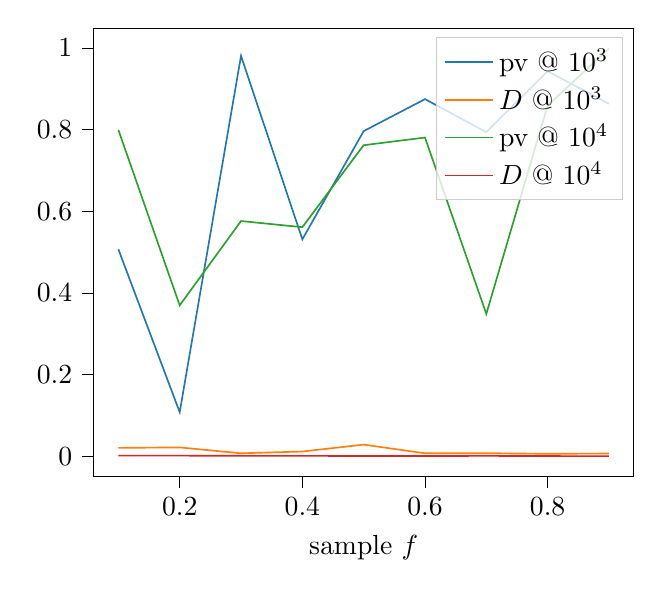
\begin{tikzpicture}

\definecolor{color0}{rgb}{0.12156862745098,0.466666666666667,0.705882352941177}
\definecolor{color1}{rgb}{1,0.498039215686275,0.0549019607843137}
\definecolor{color2}{rgb}{0.172549019607843,0.627450980392157,0.172549019607843}
\definecolor{color3}{rgb}{0.83921568627451,0.152941176470588,0.156862745098039}

\begin{axis}[
legend cell align={left},
legend style={fill opacity=0.8, draw opacity=1, text opacity=1, draw=white!80!black},
tick align=outside,
tick pos=left,
x grid style={white!69.0196078431373!black},
xlabel={sample \(\displaystyle f\)},
xmin=0.06, xmax=0.94,
xtick style={color=black},
y grid style={white!69.0196078431373!black},
ymin=-0.0494633281754976, ymax=1.0482107172787,
ytick style={color=black}
]
\addplot [semithick, color0]
table {%
0.1 0.507010806202991
0.2 0.108205629884826
0.3 0.980501661607402
0.4 0.531256191846335
0.5 0.796220592895403
0.6 0.874590263007154
0.7 0.793769479922813
0.8 0.943008434718494
0.9 0.863225066392382
};
\addlegendentry{pv @ $10^3$}
\addplot [semithick, color1]
table {%
0.1 0.0207410905979907
0.2 0.0218546127066543
0.3 0.00747578276900951
0.4 0.0117774710445298
0.5 0.0287074011071387
0.6 0.00746167076263118
0.7 0.00774003704383597
0.8 0.00624608641202262
0.9 0.00685906118737811
};
\addlegendentry{$D$ @ $10^3$}
\addplot [semithick, color2]
table {%
0.1 0.799279354556868
0.2 0.369627522511349
0.3 0.576117075259373
0.4 0.561045823324959
0.5 0.761820819160854
0.6 0.78055960545578
0.7 0.348770794064525
0.8 0.859282750488965
0.9 0.998316442485324
};
\addlegendentry{pv @ $10^4$}
\addplot [semithick, color3]
table {%
0.1 0.00165680708738947
0.2 0.00171932947696123
0.3 0.00125166550554812
0.4 0.00114222518011187
0.5 0.000885151590729216
0.6 0.000822930799605381
0.7 0.00112023913486203
0.8 0.000696684889409549
0.9 0.000430946617874794
};
\addlegendentry{$D$ @ $10^4$}
\end{axis}

\end{tikzpicture}

	\end{adjustbox}

}\caption{Stream sample}
\end{figure}


\section{Conclusion\label{sec:Conclusion}}

We studied the problem of commuting sampling with joins. In doing
so we reviewed several classical sampling techniques and modern iterations
thereof. Through our studies we discovered that the central challenge
of successfully sampling through joins is performing weighted sampling
according to frequencies of uniques values of the join attribute (in
the ``right'' operand of the join). Thus, many of the techniques
in the literature address themselves to either gathering these frequencies
or building a surrogate. In order to further investigate the join
sampling problem we implemented some of the studied techniques and
evaluated their performance (with respect to sampling accuracy) on
synthetic (but realistic data sets). We found that (with the exception
of hash join and wander join) the sampling techniques accurately produce
a uniform sampling of a join. In the future we intend to apply machine
learning approaches to the problem, such as in \cite{krishnan2019learning}.

\section{Appendix}

\subsection{Fundamental sampling algorithms\label{subsec:Stream-sampling-algorithms}}

We briefly describe some fundamental sampling algorithms that will
ultimately be employed as blackbox primitives in more sophisticated
algorithms.

\subsubsection{Rejection sampling\label{subsec:Rejection-sampling}}

Rejection sampling is a means of generating samples from some \textit{target}
\textit{distribution $p(x)$} that cannot be sampled directly but
for which we can construct a \textit{proposal distribution} $g(x)$
that encompasses the target distribution. It is based on the observation
that to sample $p(x)$, one can perform a sampling of the region under
the graph\footnote{For probability density function $p(x)$, the set of ordered pairs
$\left\{ (x,y)\mid0\leq y\leq p(x)\right\} $.} of $g(x)$, and reject all samples that fall outside of the graph
of $p(x)$. In the simplest case, the proposal distribution is a uniform
distribution $U(a,b)\times U(0,M)$, where $\left[a,b\right]$ is
the support of $p\left(x\right)$ and $M$ is the least upper bound
of $p(x)$. Then the algorithm is straightforward (see alg. \ref{alg:rejectionsampling}).
The number of samples until ``acceptance'' follows a geometric distribution
with probability $1/M$ and thus has expected number $M$. Alternatively,
more efficient algorithms exist \cite{adapativereject}.

\begin{algorithm}
\caption{Rejection Sampling}

\begin{lyxcode}
\textbf{Inputs}:~

~~target~distribution~$p\left(x\right)$~

~~with~support~$\left[a,b\right]$~and~max~$M$~

\textbf{Output}:~$\left(x,y\right)$~a~draw~from~$p$

\textbf{Init}:~$U_{1}\sim U(a,b)$,~$U_{2}\sim U(0,M)$

\textbf{Begin}:

~~while~$p\left(U_{1}\right)<p\left(U_{2}\right)$:~//~reject~if~outside

~~~~$U_{1}\sim U(a,b)$

~~~~$U_{2}\sim U(0,M)$

~~$\left(x,y\right)\coloneqq\left(U_{1},U_{2}\right)$\label{alg:rejectionsampling}
\end{lyxcode}
\end{algorithm}


\subsubsection{Reservoir sampling without replacement}

Reservoir sampling selects a simple random sample, without replacement,
of $K$ items from a population of unknown size $n$ in a single pass
over the items. The simplest such algorithm maintains a \textit{reservoir
}of size $K$ and swaps out elements according to the desired sampling
probability. See alg. \ref{alg:reservoirnaive}. This naive algorithm
runs in $O\left(n\right)$ time since it calls a random number generator
(RNG) for each element in the stream. 
\begin{algorithm}
\caption{Naive Reservoir Sampling}

\begin{lyxcode}
\textbf{Inputs}:~stream~$S$,~sample~size~$k$

\textbf{Output}:~reservoir~$A$~with~$k$~samples

\textbf{Init}:~for~$i\coloneqq1$~to~$k$:~$A[i]\coloneqq$~next$(S)$~~~

\textbf{Begin}:

~~//~replace~elements~with~gradually

~~//~decreasing~probability~~~

~~while~$S$:~~

~~~~//~randomInteger~is~inclusive~~~

~~~~$j\coloneqq$~randomInteger$(1,i)$~~~~~

~~~~if~$j\leq k$:~~~~~~~~~

~~~~~~~$A[j]\coloneqq$~next$(S)$~\label{alg:reservoirnaive}
\end{lyxcode}
\end{algorithm}

The naive algorithm can be improved upon by instead discarding elements
explicitly rather than including elements explicitly. We describe
this algorithm constructively \cite{10.1145/198429.198435}:
\begin{enumerate}
\item We conceive of naive reservoir sampling as assigning draws $u_{i}$
from $U\left(0,1\right)$ to each entry in the $S$ and then selecting
the bottom $k$ elements. This proceeds by initially filling the reservoir
and then successively replacing the largest element in the reservoir
if the $u_{i}$ associated with $s_{i}$ is smaller than the largest
element in the reservoir.
\item If fact we don't actually need to maintain the set of draws $u_{i}$
for the entire reservoir, just the largest $u_{i}$ in the reservoir.
Call that that value $\theta$.
\item The $u_{i}$ of the next $s_{i}$ to enter the reservoir is actually
distributed $U\left(0,\theta\right)$.
\item If $X_{i}\sim U(0,\theta)$ then for $Y=\max\left(X_{1},\dots,X_{k}\right)$
we have 
\[
P\left(Y\leq y\right)=\left(\frac{y}{\theta}\right)^{k}
\]
by using $P\left(X_{i}\leq x\right)=x/\theta$ and by $X_{i}$ being
i.i.d. Therefore, by using inverse CDF 
\[
U=\left(\frac{Y}{\theta}\right)^{k}\Rightarrow Y\sim\theta U^{1/k}\equiv\theta\exp\left(\frac{\log\left(U\right)}{k}\right)
\]
\item The number of elements $K$ discarded follows a geometric distribution
where the probability of success is $\theta$\footnote{Recall that the draws $u_{i}$ are drawn from $U\left(0,1\right)$
and for some $s_{i}$ to enter the reservoir it must be smaller than
the current maximum element $\theta$ and hence $P\left(X\leq\theta\right)=\theta$.}. Thus, again by using inverse CD
\[
\begin{aligned}U & =1-\left(1-\theta\right)^{K+1}\Rightarrow\\
\log\left(1-U\right) & =(K+1)\log\left(1-\theta\right)\Rightarrow\\
K & =\left\lfloor \frac{\log\left(U\right)}{\log\left(1-\theta\right)}\right\rfloor 
\end{aligned}
\]
where we use the fact that $1-U$ is also distributed $U\left(0,1\right)$.
\item We don't actually need to compare against $\theta$ but just update
it as a precursor to computing $K$.
\end{enumerate}
Thus, we can more efficiently reservoir sample by taking ``jumps''
and only querying the RNG for included elements of the stream. See
alg. \ref{alg:reservoirnaive-1}. The running time then is ${\displaystyle O(k(1+\log(n/k)))}$.

\begin{algorithm}
\caption{Optimal Reservoir Sampling}

\begin{lyxcode}
\textbf{Inputs}:~stream~$S$,~sample~size~$k$

\textbf{Output}:~reservoir~$A$~with~$k$~samples

\textbf{Init}:~

~~//~initialize~the~reservoir~

~~for~$i\coloneqq1$~to~$k$:~$A[i]\coloneqq$~next$(S)$~~

\textbf{Begin:}

~~//~note~that~$\theta=1$~since~$A$~consists

~~//~of~$k$~samples~from~$U\left(0,1\right)$.

~~//~$\mathtt{random}()$~draws~from~$U\left(0,1\right)$

~~$\theta\coloneqq$~$\exp\left(\frac{\log\left(\mathtt{random}()\right)}{k}\right)$~~

~~while~$S$:~~

~~~~$k\coloneqq\left\lfloor \frac{\log\left(U\right)}{\log\left(1-\theta\right)}\right\rfloor $

~~~~//~discard~$k$~elements

~~~~while~$S$:~next$(S)$

~~~~//~replace~random~element

~~~~//~since~we~don't~need~to~compare

~~~~$A[\mathtt{randomInteger}(1,k)]\coloneqq$~next$(S)$~\label{alg:reservoirnaive-1}

~~~~//~update~$\max$~given~that~stored~

~~~~//~element~was~drawn~from~$U\left(0,\theta\right)$

~~~~$\theta\coloneqq\theta\cdot\exp\left(\frac{\log\left(U\right)}{k}\right)$~
\end{lyxcode}
\end{algorithm}


\subsubsection{Unweighted streaming sampling with replacement\label{subsec:Unweighted-streaming-sampling}}

We present two algorithms for unweighted sequential sampling with
replacement; we omit proofs that these algorithms in fact uniformly
sample\cite{10.1145/304181.304206}. The first algorithm \texttt{BBU1}
fills the output array with copies\footnote{Whose quantity depends on a random variable drawn from a binomial
distribution.} of successive tuples from streaming relation $S$. This, in effect,
simulates sampling with replacement. The disadvantage of the alg.
\ref{alg:reservoirnaive-1-1} is that the total size $n$ of the relation
is a necessary prerequisite. Algorithm \texttt{BBU2}\textit{ }improves
on algorithm \texttt{BBU1} by eliminating that prerequisite (see alg.
\ref{alg:reservoirnaive-1-1-1}).

\begin{algorithm}
\caption{BBU1}

\begin{lyxcode}
\textbf{Inputs}:~

~~stream~$S$

~~sample~size~$k$~

~~$n\coloneqq\left|S\right|$

\textbf{Output}:~array~$A$~with~$k$~samples

\textbf{Init}:~$x\coloneqq k$,~$i\coloneqq0$~

\textbf{Begin}:

~~while~$S$~and~$x>0$:~~

~~~~$t\coloneqq$~next$(S)$~~

~~~~$X\sim B\left(x,\frac{1}{n-i}\right)$~

~~~~//~fill~$A$~with~$X$~copies~of~$t$

~~~~for~$j\coloneqq1$~to~$X$:

~~~~~~$A[i+j]\coloneqq t$~~~~\label{alg:reservoirnaive-1-1}

~~~~$x\coloneqq x-X$

~~~~$i\coloneqq i+1$
\end{lyxcode}
\end{algorithm}

\begin{algorithm}
\caption{BBU2}

\begin{lyxcode}
\textbf{Inputs}:~

~~stream~$S$

~~sample~size~$k$

\textbf{Output}:~array~$R$~with~$k$~samples

\textbf{Init}:~$N\coloneqq0$,~$A[1,\dots,k]=0$~~~~

\textbf{Begin}:

~~while~$S$:~~

~~~~$t\coloneqq$~next$(S)$~~~~

~~~~$N\coloneqq N+1$

~~~~//~set~$A[j]\coloneqq t$~with~

~~~~//~probability~$1/N$

~~~~for~$j\coloneqq1$~to~$k$:

~~~~~~$X\sim U(0,1)$

~~~~~~if~$X\leq\frac{1}{N}$:

~~~~~~~~$A[j]\coloneqq t$~~~\label{alg:reservoirnaive-1-1-1}
\end{lyxcode}
\end{algorithm}


\subsubsection{Weighted streaming sampling\label{subsec:Weighted-streaming-sampling}}

The precise semantics of weighted sampling are as such: given a streaming
relation $S$ with cardinality $n$, where each tuple $t\in S$ has
associated weight $w(t)$, a weighted, with replacement, sample is
produced by drawing $f\cdot n$ tuples with probability\footnote{Implying normalization if $\sum_{t\in S}w(t)\neq1$}
proportional to $w(t)$. We can extend algorithms \ref{alg:reservoirnaive-1-1},
\ref{alg:reservoirnaive-1-1-1} to respect these semantics; see algorithms
\ref{alg:reservoirnaive-1-1-3}, \ref{alg:reservoirnaive-1-1-4}.

\begin{algorithm}
\caption{BBWR1}

\begin{lyxcode}
\textbf{Inputs}:~

~~stream~$S$~

~~sample~size~$k$~

~~$n\coloneqq\left|S\right|$

~~weights~$w(t)$

\textbf{Output}:~array~$A$~with~$k$~samples

\textbf{Init}:~$x\coloneqq k$,~$i\coloneqq0$,~$W\coloneqq\sum_{t\in S}w(t)$~

\textbf{Begin}:

~~while~$S$~and~$x>0$:~~

~~~~$t\coloneqq$~next$(S)$~~~~

~~~~$X\sim B\left(x,\frac{w(t)}{W-i}\right)$

~~~~//~fill~$A$~with~$X$~copies~of~$t$

~~~~for~$j\coloneqq1$~to~$X$:

~~~~~~$A[i+j]\coloneqq t$~~~~\label{alg:reservoirnaive-1-1-3}

~~~~$x\coloneqq x-X$

~~~~$i\coloneqq i+w(t)$
\end{lyxcode}
\end{algorithm}

\begin{algorithm}
\caption{BBWR2}

\begin{lyxcode}
\textbf{Inputs}:~

~~stream~$S$~

~~sample~size~$k$

~~weights~$w(t)$

\textbf{Output}:~array~$R$~with~$k$~samples

\textbf{Init}:~$W\coloneqq0$,~$A[1,\dots,k]\coloneqq0$~~~~

\textbf{Begin}:

~~while~$S$:~~

~~~~$t\coloneqq$~next$(S)$~~~~

~~~~$W\coloneqq W+w(t)$

~~~~//~set~$A[j]\coloneqq t$~with~

~~~~//~probability~$w(t)/W$

~~~~for~$j\coloneqq1$~to~$k$:

~~~~~~$X\sim U(0,1)$

~~~~~~if~$X\leq\frac{w(t)}{W}$:

~~~~~~~~$A[j]\coloneqq t$~~~\label{alg:reservoirnaive-1-1-4}
\end{lyxcode}
\end{algorithm}


\subsection{Technique implementations\label{subsec:Technique-implementations}}

\begin{algorithm}
\caption{Stream Sampling}

\begin{lyxcode}
\textbf{Inputs}:~

~~$R_{1}\left(A,\dots\right),R_{2}\left(A,\dots\right)$~

~~$k\coloneqq\left\lceil f\cdot\left|R_{1}\bowtie R_{2}\right|\right\rceil $~

\textbf{Output}:~$S\equiv\mathtt{SAMPLE}_{WR}\left(R_{1}\bowtie R_{2},f\right)$

\textbf{Init:~}

~~$S[1,\dots,k]\coloneqq0$

~~$w(t)\coloneqq m_{2}\left(t.A\right)$~for~$t\in R_{1}$

\textbf{Begin}:

~~$S_{1}\coloneqq$~$\mathtt{BBWR2}\left(R_{1},k,w(t)\right)$

~~for~$i\coloneqq1$~to~$k$:~~

~~~~$t_{1}\coloneqq$~next$(S_{1})$~~~\label{alg:streamsample}

~~~~$t_{2}\sim U\left(\left\{ t\mid t\in R_{2}\wedge t.A=t_{1}.A\right\} \right)$

~~~~$S[i]\coloneqq\left(t_{1},t_{2}\right)$~~
\end{lyxcode}
\end{algorithm}

\begin{algorithm}
\caption{Group Sampling}

\begin{lyxcode}
\textbf{Inputs}:~

~~$R_{1}\left(A,\dots\right),R_{2}\left(A,\dots\right)$~

~~$k\coloneqq\left\lceil f\cdot\left|R_{1}\bowtie R_{2}\right|\right\rceil $~

\textbf{Output}:~$S\equiv\mathtt{SAMPLE}_{WR}\left(R_{1}\bowtie R_{2},f\right)$

\textbf{Init:}

~~$S[1,\dots,k]\coloneqq0$

~~$w(t)\coloneqq m_{2}\left(t.A\right)$~for~$t\in R_{1}$

\textbf{Begin}:

~~$S_{1}\coloneqq$~$\mathtt{BlackBoxWR2}\left(R_{1},k,w(t)\right)$

~~for~$i\coloneqq1$~to~$k$:~~

~~~~$t_{1}\coloneqq S_{1}[i]$~~~\label{alg:groupsample}

~~~~$t_{2}\coloneqq\mathtt{BlackBoxU2}\left(t_{1}\bowtie R_{2},1\right)$

~~~~$S[i]\coloneqq\left(t_{1},t_{2}\right)$
\end{lyxcode}
\end{algorithm}

\begin{algorithm}
\caption{Frequency Partition Sampling}

\begin{lyxcode}
\textbf{Inputs}:~\label{alg:Frequency-Partition-Sample}

~~$R_{1}\left(A,\dots\right),R_{2}\left(A,\dots\right)$,~$A\subseteq D$

~~$k\coloneqq\left\lceil f\cdot\left|R_{1}\bowtie R_{2}\right|\right\rceil $

~~//~low,~high~frequency~values~in~$R_{2}$

~~$D^{lo},D^{hi}$~

~~$R_{2}^{lo},R_{2}^{hi}\coloneqq\left.R_{2}\right|_{D^{lo}},\left.R_{2}\right|_{D^{hi}}$

~~$w_{2}(t)\coloneqq m_{2}\left(t.A\right)$~for~$t\in R_{2}^{hi}$

\textbf{Output}:~$S\equiv\mathtt{SAMPLE}_{WR}\left(R_{1}\bowtie R_{2},f\right)$

\textbf{Begin}:

~~//~stream~$R_{1}$

~~while~$R_{1}$:

~~~~//~partition~$R_{1}$

~~~~$R_{1}^{lo}\coloneqq\left.R_{1}\right|_{D^{lo}}$~

~~~~$R_{1}^{hi}\coloneqq\left.R_{1}\right|_{D^{hi}}$

~~~~//~sample~but~also~collect~

~~~~//~stats~$w_{1}\left(t\right)$~on~$R_{1}^{hi}$

~~~~$S_{1},w_{1}\left(t\right)\coloneqq$~$\mathtt{BBWR2}\left(R_{1}^{hi},k,w(t)\right)$

~~//~integrate/combine~stats~

~~$w\left(t\right)\coloneqq w_{1}\left(t\right)\cup w_{2}\left(t\right)$

~~//~from~$w\left(t\right)$~you~can~approximate

~~$n_{hi}\coloneqq\left|R_{1}^{hi}\bowtie R_{2}^{hi}\right|$

~~$R_{1}^{*}\coloneqq S_{1}\cup R_{1}^{lo}$

~~//~stream~join

~~while~$J^{*}\coloneqq R_{1}^{*}\bowtie R_{2}$:

~~~~$n_{lo}\coloneqq\left.J^{*}\right|_{D^{lo}}$~//~i.e.~$n_{lo}\coloneqq\left|R_{1}^{lo}\bowtie R_{2}^{lo}\right|$

~~~~//~partition~$J^{*}$~

~~~~$J^{lo}\coloneqq\mathtt{BBU2}\left(\left.J^{*}\right|_{D^{lo}},k\right)$~

~~~~//~$S_{1}\equiv\left\{ s_{i}\right\} $~and~just~

~~~~//~like~in~Group-Sample

~~~~$J^{hi}\coloneqq\mathtt{BBU2}\left(s_{i}\bowtie\left.J^{*}\right|_{D^{hi}},k\right)$

~~//~\#~of~heads~and~tails

~~//~$p=\frac{n_{hi}}{n_{lo}+n_{hi}},1-p=\frac{n_{lo}}{n_{lo}+n_{hi}}$

~~$k_{lo},k_{hi}\coloneqq B\left(k,p\right)$~~~

~~$S^{lo}\coloneqq\mathtt{BlackBoxUWoR2}\left(J^{lo},k_{lo}\right)$

~~$S^{hi}\coloneqq\mathtt{BlackBoxUWoR2}\left(J^{hi},k_{hi}\right)$

~~$S\coloneqq S^{lo}\cup S^{hi}$
\end{lyxcode}
\end{algorithm}

\begin{algorithm}
\caption{Count Sampling}

\begin{lyxcode}
\textbf{Inputs}:~

~~$k$

~~$R_{2}\left(A,\dots\right)$

~~$S_{1}\subseteq R_{1}^{hi}$

\textbf{Output}:~$S\equiv\left(S_{1}\bowtie R_{2}^{hi}\right)$

Init:

~~$H$~//~hash~table~for~counting

\textbf{Begin}:

~~while~$S_{1}$:

~~~~$t\coloneqq\mathtt{next}\left(S_{1}\right)$

~~~~//~count~number~of~tuples~such~that

~~~~//~$t.A=v$

~~~~$H[t.A]\coloneqq H[t.A]+1$~~~

~~//~sample~$S_{2}\subseteq R_{2}$~such~that~

~~//~the~number~of~tuples~$t$~with

~~//~$t.A\equiv v$~is~exactly~$v$

~~while~$S_{2}\coloneqq$~$\mathtt{BBWR2}\left(R_{2},H\right)$:

~~~~$t_{1}\coloneqq\mathtt{next}\left(S_{2}\right)$~~~\label{alg:count-sample}

~~~~$t_{2}\coloneqq\mathtt{BlackBoxWoR}\left(t_{1}\bowtie S_{1},1\right)$

~~~~$S[i]\coloneqq\left(t_{1},t_{2}\right)$
\end{lyxcode}
\end{algorithm}

\bibliographystyle{plain}
\bibliography{biblio}

\end{document}
